% Disable the default assymmetric margins of twoside.

\documentclass[twoside]{book}

\usepackage[fontsize=12]{scrextend}
\usepackage{graphicx}
\usepackage{caption}
%\usepackage[figuresright]{rotating}

\usepackage{fancyhdr}
\setlength{\headheight}{15pt}

\usepackage[paperwidth=5.5in,paperheight=8.5in,top=0.8in,bottom=0.75in,left=0.5in,right=0.5in]{geometry}

\title{Bookbinding}
\author{Paul N. Hasluck}
\date{1903}

\begin{document}

%\extrafloats{1000} % To keep placing figures after errors.

% No visible numbering on sections.
\setcounter{secnumdepth}{0}

% Set up headers and footers using fancyhdr.
\fancyhf{}
\renewcommand{\headrulewidth}{0pt} % Remove line under header text.
\fancyhead{}
\fancyfoot{}

% Set up the ordinary page style,
% which happens to be named "fancy"
% because we're using fancyhdr.
\pagestyle{fancy}
\parindent=12pt
\parskip=0pt

% The pagenumbering can't be set on a style?
\pagenumbering{arabic}
\setcounter{page}{3}

\vspace*{\fill}

% The title page.

\begin{center}

\begin{Huge}
BOOKBINDING
\end{Huge}

\vspace*{\fill}

\textit{WITH NUMEROUS ENGRAVINGS AND DIAGRAMS}

\vspace*{\fill}

\begin{small}EDITED BY\end{small} \\

\begin{Large}
PAUL N. HASLUCK
\end{Large}
\\

\begin{tiny}
EDITOR OF "WORK" AND "BUILDING WORLD," \\
AUTHOR OF "HANDYBOOKS FOR HANDICRAFTS," ETC. ETC.
\end{tiny}

\vspace*{\fill}

\textit{PHILADELPHIA}

\begin{Large}DAVID MCKAY,\end{Large} PUBLISHER

1022, \textit{MARKET STREET}

1903

\end{center}

\vspace*{\fill}

\pagebreak

% blank page after title
\vspace*{\fill}
\pagebreak

\pagestyle{empty} % Turn off headers and footers.

\vspace*{\fill}

\begin{center}

\begin{Large}
PREFACE.
\end{Large}

\rule{0.5cm}{1pt.}

\end{center}

\noindent This Handbook contains, in a form convenient for
everyday use, a comprehensive digest of the information
on Bookbinding, scattered over nearly twenty
thousand columns of WORK--one of the weekly journals
it is my fortune to edit--and supplies concise
information on the details of the subjects of which it
treats.

In preparing for publication in book form the mass
of relevant matter contained in the volumes of
WORK, much had to be arranged anew, altered, and
largely rewritten. The contributions of many are so
blended that the writings of individuals cannot be
distinguished for acknowledgment. A large part of the
contents was written by the Foreman Bookbinder
in a London firm, and the substance of a series of
articles written by Mr. Wm. Norman Brown has also
been incorporated.

Readers who may desire additional information
respecting special details of the matters dealt with
in this Handbook, or instructions on kindred subjects,
should address a question to WORK, so that it may
be answered in the columns of that journal.\\

\begin{flushright}P. N. HASLUCK. \\ \end{flushright}

\noindent
\textit{La Belle Sauvage, London.}\\
\textit{November, 1902.}

\vspace*{\fill}

\pagebreak

% Table of contents.

\vspace*{\fill}

\begin{center}\begin{Large}CONTENTS.\end{Large}\end{center}

\begin{center}\rule{0.5cm}{1pt.}\end{center}

\begin{tabular}{r l r}
    I. & Bookbinders' Appliances\dotfill & 9 \\
\\
   II. & Folding Printed Book Sheets\dotfill & 33 \\
\\
  III. & Beating and Sewing\dotfill & 38 \\
\\
  IV. & Rounding, Backing, and Cover Cutting\dotfill & 48 \\
\\
   V. & Cutting Book Edges\dotfill & 55 \\
\\
  VI. & Covering Books\dotfill &                                 58 \\
\\
 VII. & Cloth-bound Books, Pamphlets, etc.\dotfill &             66 \\
\\
VIII. & Account Books, Ledgers, etc.\dotfill &                   72 \\
\\
  IX. & Colouring, Sprinkling, and Marbling Book Edges\dotfill & 79 \\
\\
   X. & Marbling Book Papers\dotfill &                           92 \\
\\
  XI. & Gilding Book Edges\dotfill &                            101 \\
\\
 XII. & Sprinkling and Tree Marbling Book Covers\dotfill &      110 \\
\\
XIII. & Lettering, Gilding, and Finishing Book Covers\dotfill & 115 \\
\\
&      Index\dotfill                                          &156
\end{tabular}

\pagebreak

\vspace*{\fill}

\begin{center}\begin{Large}LIST OF ILLUSTRATIONS.\end{Large}\end{center}

\begin{center}\rule{0.5cm}{1pt.}\end{center}

\begin{tiny}

\begin{tabular}{r l r r l r }
FIG.  & & PAGE                              &   FIG. &                                    & PAGE. \\
1.     & Beating Hammer            \dotfill & 10     &    44. & Book with Square Lettering           &     \\ 
2.     & Standing Press            \dotfill & 11     &        & Pieces                      \dotfill &  62 \\ 
3.     & Simple Press              \dotfill & 12     &    45. & Book with Oval Lettering             &     \\ 
4.     & Sewing Press              \dotfill & 13     &        & Piece                       \dotfill &  63 \\ 
5-8.   & Details of Home-made               &        &    46. & Book with Lettering Piece            &     \\ 
       & Sewing Press              \dotfill & 14     &        & at the Head                 \dotfill &  63 \\ 
 9.    & Sewing Press              \dotfill & 15     &    47. & Side of Cover of Half-               &     \\ 
10.    & Sewing Press              \dotfill & 16     &        & bound Book                  \dotfill &  65 \\ 
11.    & Lying Press               \dotfill & 16     &    48. & Sprayer for Colouring Book           &     \\ 
12.    & Lying Press               \dotfill & 17     &        & Edges                       \dotfill &  80 \\ 
13.    & Lying Press and Plough    \dotfill & 18     &    49. & Marbling Comb               \dotfill &  82 \\ 
14.    & Cramping Screw for Lying           &        &    50. & Marbling Comb               \dotfill &  83 \\ 
       & Press                     \dotfill & 18     &    51. & Marbling Comb               \dotfill &  84 \\ 
15.    & Combined Lying Press and           &        &    52. & Marbling Trough             \dotfill &  84 \\ 
       & Box                       \dotfill & 20     &    53. & Marbling Trough and                  &     \\ 
16-17. & Details of Home-made               &        &        & Colour Pots                 \dotfill &  85 \\ 
       & Plough                    \dotfill & 21     &    54. & Marbling Book Edges         \dotfill &  89 \\ 
18.    & Elevation of Home-made             &        &    55. & Nonpareil Marble            \dotfill &  93 \\ 
       & Plough                    \dotfill & 22     &    56. & Reversed Nonpareil Marble   \dotfill &  94 \\ 
19.    & Plan of Home-made Plough  \dotfill & 22     &    57. & Wave Nonpareil Marble       \dotfill &  95 \\ 
20.    & Wedges and Chisel of               &        &    58. & Fancy Dutch Marble          \dotfill &  96 \\ 
       & Home-made Plough          \dotfill & 23     &    59. & Italian Marble              \dotfill &  96 \\ 
21.    & Plough                    \dotfill & 25     &    60. & Dutch Antique Marble        \dotfill &  97 \\ 
22.    & Sliding Block for Plough  \dotfill & 25     &    61. & Antique Spot Marble         \dotfill &  97 \\ 
23.    & Plough Knife              \dotfill & 27     &    62. & West End Marble             \dotfill &  98 \\ 
24.    & Plough                    \dotfill & 27     &    63. & Machine-pattern Marble      \dotfill &  99 \\ 
25.    & Strawboard Cutter         \dotfill & 30     &    64. & Gilder's Press              \dotfill & 102 \\ 
26.    & Gauge of Strawboard                &        &    65. & Steel Scraper for Book Edges\dotfill & 102 \\ 
       & Cutter                    \dotfill & 31     &    66. & Gilder's Cushion            \dotfill & 103 \\ 
27.    & Clamp of Strawboard                &        &    67. & Gilder's Knife              \dotfill & 104 \\ 
       & Cutter                    \dotfill & 32     &    68. & Gilder's Knife              \dotfill & 104 \\ 
28.    & Printed Book Sheet        \dotfill & 35     &    69. & Gilder's Tip                \dotfill & 105 \\ 
29.    & Printed Sheet, First Fold \dotfill & 35     &    70. & Gilder's Burnisher          \dotfill & 105 \\ 
30.    & Printed Sheet, Second              &        &    71. & Sprinkling on Panels        \dotfill & 111 \\ 
       & Fold                      \dotfill & 35     &    72. & Book between Marbling                &     \\ 
31.    & Printed Sheet, Third Fold \dotfill & 35     &        & Rods                        \dotfill & 113 \\ 
32.    & Saw Kerfs in Back of Book \dotfill & 41     &    73. & Finisher's Press            \dotfill & 116 \\ 
33.    & Sewing Book               \dotfill & 43     &    74. & Finisher's Stove            \dotfill & 116 \\ 
34.    & Method of Sewing Book              &        &    75. & Fillet                      \dotfill & 117 \\ 
       & "Two on"                  \dotfill & 45     &    76. & Lines made with Fillets     \dotfill & 117 \\ 
35.    & Method of Backing Book    \dotfill & 49     &    77. & Lines made with Fillets     \dotfill & 117 \\ 
36.    & Book and Backing Boards            &        &    78. & Pallet                      \dotfill & 117 \\ 
       & in Lying Press            \dotfill & 51     & 79-84. & Pallet Patterns             \dotfill & 118 \\ 
37.    & Scratching- up Tool       \dotfill & 53     &    85. & Line Tools                  \dotfill & 118 \\ 
38.    & Book Tied up for Cutting  \dotfill & 57     & 86-87. & Line Tools                  \dotfill & 119 \\ 
39.    & Tightening Leather on              &        &    88. & Lines made with Gouges      \dotfill & 119 \\ 
       & Back of Book              \dotfill & 59     &    89. & Lines made with Gouges      \dotfill & 119 \\ 
40.    & Turning in Leather at Head         &        &    90. & Small Finishing Tool        \dotfill & 120 \\ 
       & and Tail of Book          \dotfill & 60     &    91. & Corner Pattern              \dotfill & 120 \\ 
41.    & Turning in Corners of              &        &    92. & Corner Pattern              \dotfill & 120 \\ 
       & Leather                   \dotfill & 61     &    93. & Centre Patterns             \dotfill & 120 \\ 
42.    & Section through Head Band          &        &    94. & Centre Patterns             \dotfill & 120 \\ 
       & and Cap                   \dotfill & 61     & 95-98. & Cover Ornaments             \dotfill & 121 \\ 
43.    & Book Tied up in Boards    \dotfill & 61     &    99. & Finished Back of Book       \dotfill & 121 \\ 

\end{tabular}

\pagebreak

\begin{tabular}{r l r r l r }

FIG. &                                      & PAGE  & FIG. &                                         & PAGE \\
100. & Letter Holder               \dotfill &   123 & 115. & Part Border of Cover Design  \dotfill & 140 \\
101  & Devil for Preparing Glaire  \dotfill &   124 & 116. & Part Inside Border of Cover             &     \\
102. & Polisher                    \dotfill &   125 &      & Design                         \dotfill & 140 \\
103. & Polisher                    \dotfill &   125 & 117. & Corner of Cover Design         \dotfill & 141 \\
104. & Method of Holding Letter-            &       & 118. & Inside Corner of Cover Design  \dotfill & 141 \\
     & ing Tool                    \dotfill &   128 & 119. & Tray or Force                  \dotfill & 143 \\
105. & Method of Applying Pallet   \dotfill &   129 & 120. & Part Design of Hand-tooled              &     \\
106. & Method of Spacing Letters   \dotfill &   130 &      & Morocco Cover                  \dotfill & 147 \\
107. & Scale for Spacing Letters   \dotfill &   130 & 121. & Part Design of Hand-tooled              &     \\
108. & Type Holder                 \dotfill &   131 &      & Morocco Cover                  \dotfill & 149 \\
109. & Back of Book                \dotfill &   133 & 122. & Part Design of Hand-tooled              &     \\
110. & Lettering Press             \dotfill &   137 &      & Morocco Cover                  \dotfill & 151 \\
111. & Heater Box                  \dotfill &   137 & 123. & Hand-tooled Morocco Cover               &     \\
112. & Blocking Plate              \dotfill &   137 &      & of Bible                       \dotfill & 153 \\
113. & Half Design for Album                &       & 124. & First Pressing with Grain-              &     \\
     & Cover                       \dotfill &   138 &      & ing Plate                      \dotfill & 155 \\
114. & Half Design for Album       \dotfill &       & 125. & Second Pressing with                    &     \\
     & Cover                       \dotfill &   139 &      & Graining Plate                 \dotfill & 155 \\

\end{tabular}

\end{tiny}

\pagebreak

\thispagestyle{empty}

% Content begins.

\pagestyle{fancy}
\fancyhead[LE,RO]{\thepage}\fancyhead[CE]{\textit{BOOKBINDING.}}

\fancyhead[CO]{\textit{BOOKBINDER'S APPLIANCES.}}

\thispagestyle{empty}

\vspace*{\fill}

\begin{center}

\begin{Huge}BOOKBINDING. \\ \end{Huge}

\begin{center}\rule{0.5cm}{1pt.}\end{center}

\begin{large}CHAPTER I.\end{large}

\begin{small}BOOKBINDERS' APPLIANCES.\end{small}

\end{center}

\noindent
Bookbinding is a term that is popularly applied to
any process for making a book by fastening together
printed or unprinted sheets of paper, and providing
them in this compact form with a suitable
covering. The term, used in this sense, covers
such widely different productions as a cheap cloth
or paper-covered novel and a costly volume bound
in leather. These two books are representative
products of the two great divisions of the bookbinding
industry as carried on at the present day. Each
division may, indeed, almost be called a distinct
industry; for, though the means employed and the
results obtained in both cases bear on the surface
a certain resemblance to each other, the manner in
which the work is carried out, and the result aimed
at, are in both cases fundamentally different.

A bound book is, technically, a book bound in
leather. It is more solid in appearance, is better
sewn, the leaves lie more compactly together, and
the book opens more readily than a cloth-boarded
book. Even a person without any technical knowledge
is struck with the difference between a
leather-bound volume and a cloth-boarded book.
While the former will last for years and resist hard
usage, the latter serves a temporary purpose only,
and rough usage soon reduces it to a collection of
loose leaves, scarcely held together by a few tangled
threads. Belonging also to the division of bound
\pagebreak
books are half-bound books, of which the back may
be of leather, or of cloth or other material used in
place of leather, and the sides of cloth or paper.
Other minor but not unimportant differences that
distinguish bound books from cloth-boarded books
will be explained in due course.

The tools used in bookbinding first will be described.
A cloth-boarded book can be produced
with the same tools (though less in number) that
are employed for a leather-bound volume, but the
latter cannot be produced with the appliances used.
for the former.

Before beginning the study of this subject, the
amateur is advised to obtain two old leather-bound
	\begin{figure}[h]
		\centering
		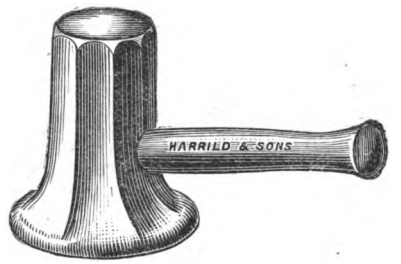
\includegraphics[width=0.6\textwidth]{Figures/_001.png}
		\caption*{Fig. 1.--Beating Hammer.}
	\end{figure}
books. Take one of these books to pieces carefully,
bit by bit; and whilst doing so note every
contrivance used for holding the book together, and
frequently compare the partially dissected book with
the other volume, which should be kept intact. The
value of this object lesson will be realised when
making the first attempt at binding a book.

A book may be bound by the amateur with the
aid of comparatively few and simple tools. It has
not, therefore, been thought necessary to describe
here the many more or less expensive machines and
appliances at present used in bookbinding. Leather
binding is largely done by hand, the material \pagebreak
employed, the manner in which the work is done, and
the limited demand for leather compared with cloth
books, precluding the use of machinery to any
considerable extent. On the other hand, the binding
of cloth-boarded books is considerably helped, and,
in some cases, almost wholly done, by machinery;
because cloth books must be produced rapidly, and
in large numbers (often tens of thousands, all of one
size and pattern), and at a comparatively low cost.
The following are some of the tools that will be
required for leather binding:
	\begin{figure}[h]
		\centering
		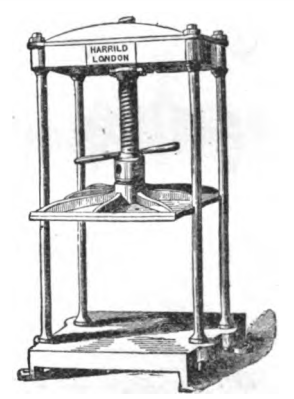
\includegraphics[width=0.4\textwidth]{Figures/_002.png}
		\caption*{Fig. 2.--Standing Press.}
	\end{figure}
The folder or folding-stick is a piece of flat bone,
about 6 in. long and rather more than 1 in. wide,
with rounded ends. The folder, as its name implies,
is used for folding into page size the printed sheets
received from the printer.

The beating hammer and stone are adjuncts of
an old-fashioned bookbinder's shop, and have been
replaced by the rolling machine. The amateur,
however, unless he can get his work rolled for him,
must use the beating hammer, and he should endeavour
to obtain one that has been specially made
\pagebreak
for the purpose. The beating hammer weighs from
10 lb. to 12 lb., is more or less bell-shaped, and has a
short handle (see Fig. 1, p. 10). A stone or iron slab
will also be required. The slab must be level and
perfectly smooth, and it should be firmly bedded.
When not in use the surface of the slab should be
kept covered. It will be found convenient to bed the
slab in a box of sand, and to provide the box with
a cover.

The standing press is used to compress books
during the process of binding, and there are several
	\begin{figure}[h]
		\centering
		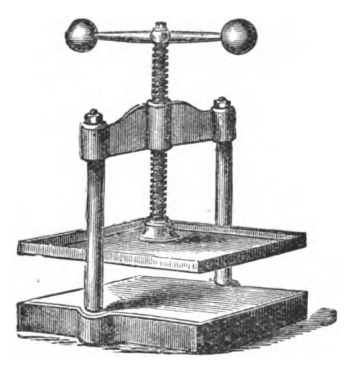
\includegraphics[width=0.5\textwidth]{Figures/_003.png}
		\caption*{Fig. 3.--Simple Press.}
	\end{figure}
different forms of it. The typical standing press
(Fig. 2, p. 11) consists of vertical pillars, a long stout
screw, a platen, and the bed. A letter-copying
press represents, roughly and on a small scale, a
bookbinder's standing press, but in the bookbinder's
press the power is applied by a long iron bar that
is inserted in holes drilled in a ball of iron that
forms the bottom of the screw. The folded sections
of the book are piled upon the bed of the press,
and the platen is screwed down as tightly as
possible by the combined strength of two or more men.
A stout copying press, however, can be used \pagebreak
for bookbinding on a small scale, smooth slabs of
iron or hard wood called pressing boards, not less
than the size of the book, being placed between
each three or four sections. Or, if a copying press
or similar contrivance is not available, heavy
weights may be laid on the folded sheets, and the
pressure continued for twenty-four hours, or longer
if necessary. A small press, like that shown by
	\begin{figure}[h]
		\centering
		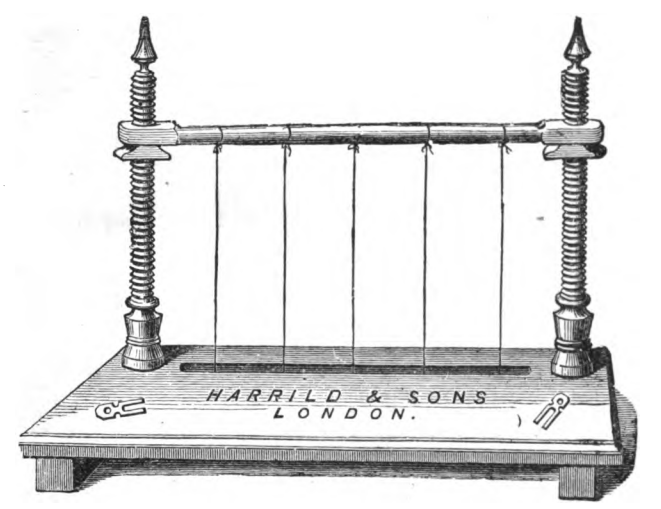
\includegraphics[width=\textwidth]{Figures/_004.png}
		\caption*{Fig. 4.--Sewing Press.}
	\end{figure}
Fig. 3, sometimes may be bought second-hand, and
would be a valuable acquisition. The pressing
boards should be of some hard wood, generally
beech, planed perfectly smooth on both surfaces,
and rectangular in shape. Iron plates sometimes
are used.

The sewing press is not a press in the modern
sense of the term, as it is not used for purposes of
compression; it is a contrivance by which the bands
\pagebreak
or cords upon which a book is sewn are kept at
tension and in their proper places, while the sections
or sheets of a book are sewn to them. The usual
form of the sewing press is shown by Fig. 4, p. 13,
and its use will be described later. In Fig. 4 are
shown the keys employed to hold down the cords.

A home-made sewing press is illustrated by Fig.
5. The bottom board A may be made of 1-in. stuff,
1 ft. 9 in. long by 1 ft. broad, with uprights C, 10 in.
high by 1-1/4 in. by 3/4 in. The top piece B, shown
separately in Fig. 6, should be of 1-in. oak, 2 ft.
3 in. long, 1 in. square, with corners rounded, and
	\begin{figure}[h]
		\centering
		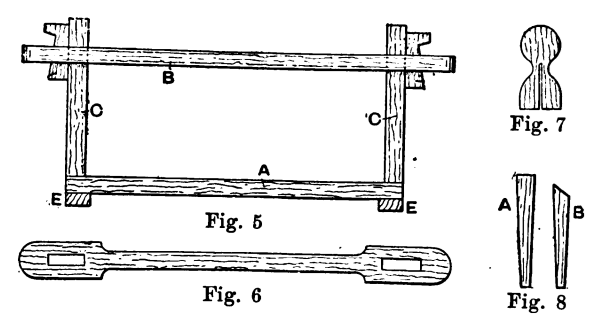
\includegraphics[width=0.8\textwidth]{Figures/_005-008.png}
		\caption*{Figs. 5 to 8.--Details of Home-Made Sewing Press.}
	\end{figure}
2-1/4 in. wide at the ends. The cross-pieces E
underneath measure 1-1/2 in. by 3/4 in. The uprights can be
either hinged or fixed with iron plates screwed on
from outside. The key (Fig. 7) is of 3/8-in. ash, cut
to the shape shown, 2-1/2 in. long, 1-1/4 in. wide, and
1/2 in. wide in the middle, and with a saw-cut for the
string. Three keys are wanted. The cutting and
backing boards (sections of which are shown at A
and B in Fig. 8) can be 1 ft. 3 in. long by 3-1/2 in. wide.

Another sewing press is shown by Fig. 9. It is
simply a flat bottom with two screwed uprights,
and cross-bar with nuts below for the purpose of
keeping the bands or strings tight while the book is
\pagebreak
being sewn. The slit immediately below the crossbar
and between the uprights allows of strings going
through and being fastened on the bottom with a
tack or anything handy. A wooden screw upright is
preferable, and the ends need not be glued into
the bottom, but fitted so that they can be taken out
for convenience, and the whole stowed away in
small compass. Differing only in detail is the
sewing press illustrated by Fig. 10, p. 16.

The lying press (Fig. 11, p. 16) (more commonly
called the laying press) may also be termed the
	\begin{figure}[h]
	\centering
	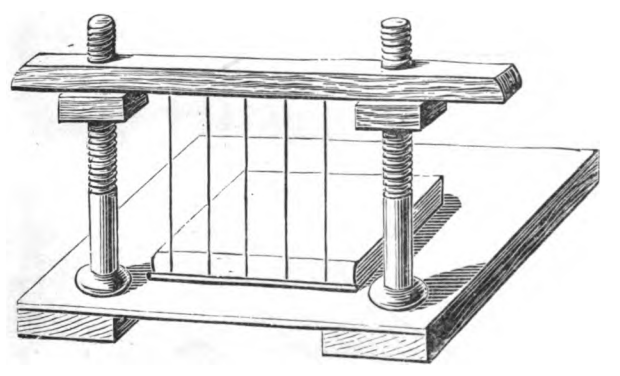
\includegraphics[width=0.8\textwidth]{Figures/_009.png}
	\caption*{Fig. 9.--Sewing Press.}
	\end{figure}
backing press and the cutting press, as both the
operations of backing a book and of cutting the edges
are performed at it. For cutting, is kept uppermost the
side that has on the left cheek the two guide rods
between which the plough works, as shown at Fig.
12, p. 17. For backing, the press is turned over,
and the plain sides of the cheeks are placed uppermost.
This press is worked by a short unattached
iron press pin.

A lying press of slightly different construction is
illustrated by Fig. 13, p. 18, which shows a plough,
\pagebreak
A, in position also. The construction of this
particular plough will be dealt with later. This press
consists of six essential parts--two boards, two screws,
	\begin{figure}[h]
		\centering
		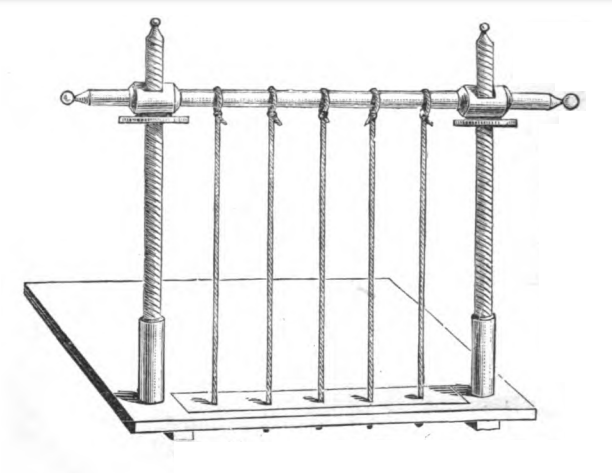
\includegraphics[width=0.7\textwidth]{Figures/_010.png}
		\caption*{Fig. 10.--Sewing Press.}
	\end{figure}
	\begin{figure}[h]
		\centering
		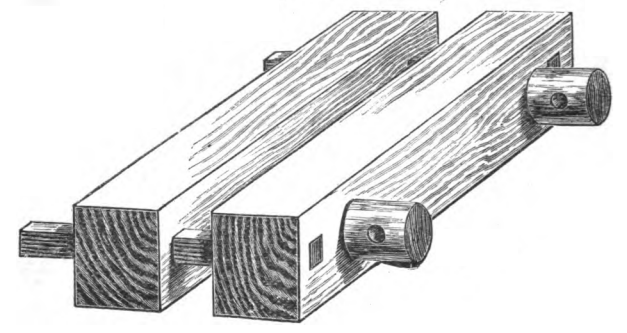
\includegraphics[width=0.7\textwidth]{Figures/_011.png}
		\caption*{Fig. 11.--Lying Press.}
	\end{figure}
and two drilled and tapped handles. To make it,
first procure a piece of board 18 in. long, 6 in.
broad, and 1-1/2 in. thick; then get another one of
the same length and thickness, but only 5-1/2 in.
broad. Plane these perfectly true and fasten
\pagebreak
together temporarily, with two faces together and
one long edge of each piece flush with that of the
other, and bore a hole right through for the screw,
which must now be made. The screw may be of
wood, similar to the screw of a carpenter's vice; but
an iron one answers the purpose quite as well.
Threaded pieces of iron wire (3/8 in. or 5/16 in.), about
8 in. long, have one end each screwed into a plate
of iron 1 in. or 2 in. across, either round or square,
	\begin{figure}[h]
		\centering
		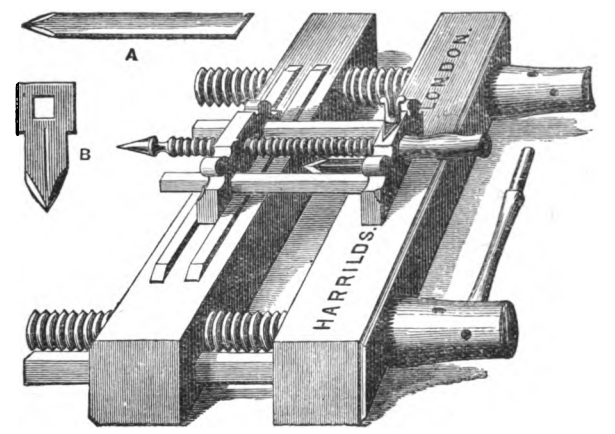
\includegraphics[width=\textwidth]{Figures/_012.png}
		\caption*{Fig. 12.--Lying Press.}
	\end{figure}
and about 1/8 in. thick (see Fig. 14, p. 18); the end of
the screw is burred over to hold more firmly. The
iron or brass handles are tapped sufficiently large to
allow them to be screwed on with comparative
ease; a lever on each one enables sufficient power
to be obtained to press the books well together.
Having fitted together the parts of the screw, take
off the handles, and pass the screw through the
back board, and fasten it in place by passing small
screws through the holes in the plate. These screws
will keep the large screw from slipping backwards
\pagebreak
	\vspace*{\fill}
	\begin{figure}[h]
		\centering
		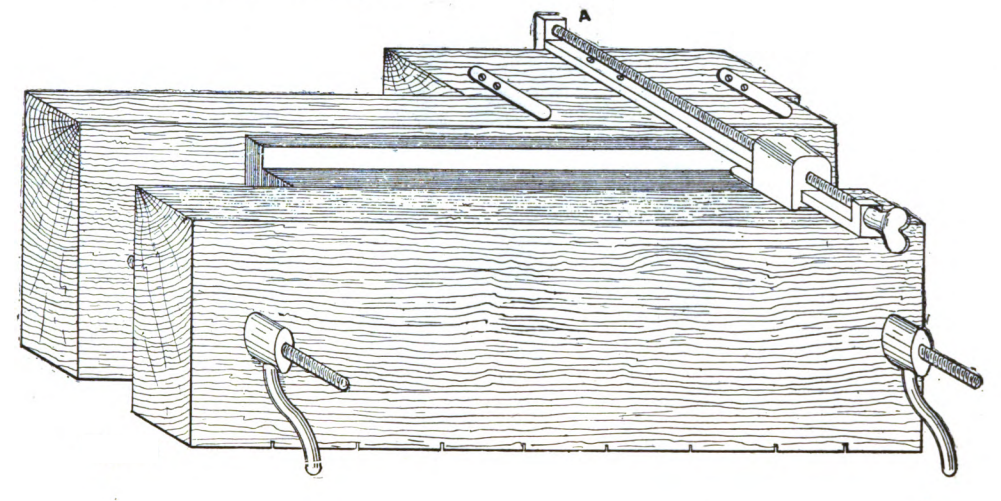
\includegraphics[width=0.8\textwidth]{Figures/_013.png}
		\caption*{Fig. 13.--Lying Press and Plough.}
	\end{figure}
	\vspace*{\fill}
	\begin{figure}[h]
		\centering
		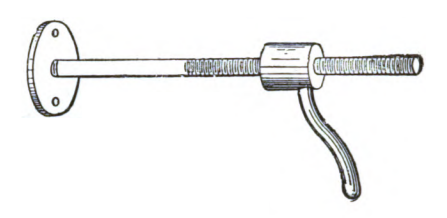
\includegraphics[width=0.8\textwidth]{Figures/_014.png}
		\caption*{Fig. 14.--Clamping Screw for Lying Press.}
	\end{figure}
	\vspace*{\fill}
\pagebreak
and forwards, and also from turning round while
the press is in use. Now put on the front and screw
the boards together with the handles. Turn the
press over so as to have the edges that are level
uppermost, and then with a broad-set saw cut
notches about 1/4 in. deep at intervals of about 2 in.
apart right across the two boards, as shown at the
bottom of Fig. 13. The lying press itself is complete,
but for convenience is attached to a support
which serves as a guide to keep the books perfectly
level while arranging them for binding. To make
the support, procure a piece of board about 3/4 in.
thick and 14 in. by 12. in., and a piece of 1-in. board
14 in. by 8 in., and screw them together at right
angles by their longer edges. The press is supported
on the larger piece, the 14-in. by 8-in. piece
standing upright on edge. On top of the back board
of the press is laid a piece of wood 5 in. by 14 in.
by 1-1/2 in., and this is screwed to the upright back
of the support to form a continuation of the back
board of the press.

It has been remarked that a press must have a
good support if required to work with convenience.
So many things are done with this appliance--pressing,
cutting, backing, screwing-out, screwing-in,
etc.--that as it is not very heavy it is always
shifting on the table or bench, and thus causing trouble.
To remedy all these inconveniences, one method is
to make a combined press and box. In a box from
2 ft. 6 in. to 3 ft. long, 2 ft. wide, and 2 ft. deep,
fix two pieces of beech wood (5 in. by 4 in.) A and B
(Fig. 15, p. 20) of the same length as the inside
measurement of box. The wood must be planed straight
and squared up; bore holes for the screws C, say
1-1/4 in. diameter. Inside the box, on ends, nail two
bars of wood D (as shown by dotted lines in Fig.
15), 5 in. from top, so that the front and back
pieces of the press, when placed on them, will come
level with the top of the box. Obtain iron screws
\pagebreak
and nuts to fit, say 1 in. or 1-1/4 in. diameter, of the
shape shown at C, and on the nuts have tails with
two holes for screw-nails to fasten into the press
bar, cutting a hole in the wood so that the nut may
be inserted flat.

	\begin{figure}[h]
		\centering
		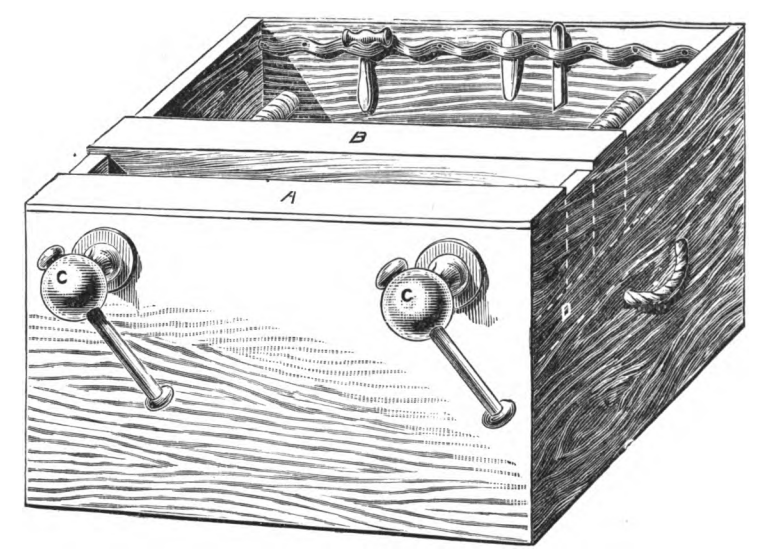
\includegraphics[width=\textwidth]{Figures/_015.png}
		\caption*{Fig. 15.--Combined Lying Press and Box.}
	\end{figure}

The plough is the implement by which ordinarily
the edges of well-bound books are cut. The plough
consists of a couple of wooden cheeks, which can be
brought together or drawn apart by rotating the
handle and screw. To the bottom of the right cheek
\pagebreak
is fixed a plough knife, which is a blade of well-
tempered steel secured to the under surface of the
right-hand cheek of the plough by a screwed bolt and nut.
Fig. 12 shows the plough as it lies ready for use in the
cutting press. The book is carefully screwed up in
the press, and the edges of the book are cut by
sliding the plough forwards and backwards. The
guiding groove on the plough is on the left-hand
side of the press. On the right-hand side of the
plough is a handle that turns the screw by which
the knife is pushed laterally across the edges of
the book every time the plough is thrust forward.
Plough knifes are shown at A and B, Fig. 12, p. 17.

	\begin{figure}[h]
		\centering
		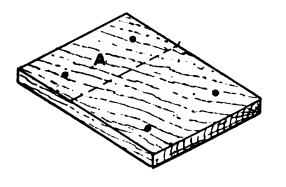
\includegraphics[width=0.45\textwidth]{Figures/_016.png}
		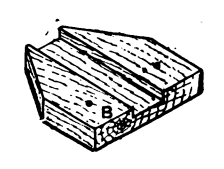
\includegraphics[width=0.45\textwidth]{Figures/_017.png}
		\caption*{Figs. 16 and 17.--Details of Home-made Plough.}
	\end{figure}

Home-made ploughs are serviceable tools, and
can be constructed from simple material, such as a
chisel, some pieces of wood, and a few screws.
Knock off the handle from an ordinary 1/2-in. chisel
having a "shoulder" near the haft, and replace it
with a cork; cut to the shape of Fig. 16 a piece of
thin wood (say 1/4 in. thick) 2-1/2 in. in breadth, its
length depending on the length of the chisel. Place
the chisel on the wood so that the cutting end overhangs
about 1-5/8 in.; at the other end mark where
the shoulder of the chisel touches the wood, and cut
across just above the mark so that the shoulder falls
over the edge and allows the chisel to lie flat on
the wood. Cut another piece of wood thicker than
the last (of full 1/2-in. stuff) to the shape of Fig. 17.
\pagebreak
This will be, say, 2-1/2 in. in breadth, 1-1/4 in. along its
parallel sides, and 2-1/2 in. in extreme length. Cut a
groove down the middle as wide as the widest part
of the chisel and as deep generally as the chisel is
thick, but a little deeper than this towards the end
	\begin{figure}[h]
		\centering
		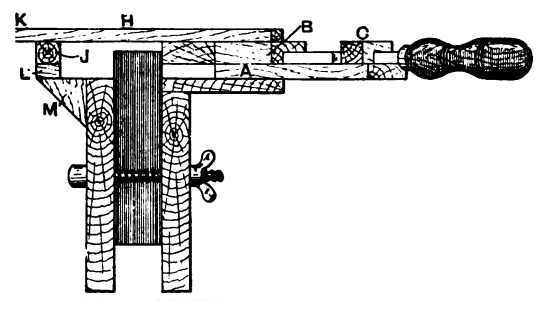
\includegraphics[width=0.7\textwidth]{Figures/_018.png}
		\caption*{Fig. 18.--Elevation of Home-made Plough.}
	\end{figure}	
	\begin{figure}[h]
		\centering
		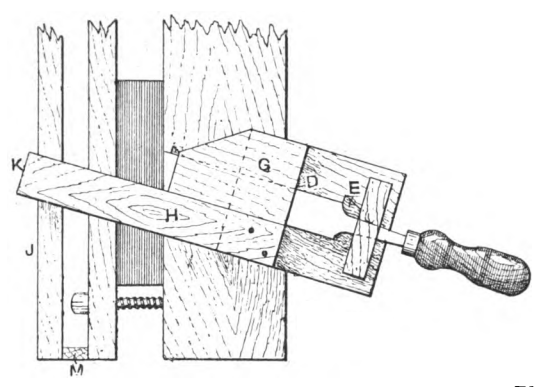
\includegraphics[width=0.7\textwidth]{Figures/_019.png}
		\caption*{Fig. 19.--Plan of Home-made Plough.}
	\end{figure}
B. Put the second piece of wood, groove downwards,
on the first one so that the square end B of
Fig. 17 rests upon the portion marked A of Fig. 16,
allowing the pointed end to overhang. Screw the
two pieces together from underneath, taking care
\pagebreak
to countersink the screw-heads. In the tunnel thus
formed insert the chisel with its bevelled edge upwards.
as it must always be when in use, and see that it
has a rather loose fit. If it is all right, the cutting
edge will project about 3/8 in. at one end, and the
shoulder will just fall over the edge at the other
end. In a piece of wood C (Fig. 18), measuring,
say, 2 in. by 1/2 in. by 1/2 in., make a groove of the
same width as before, but a trifle deeper than the
groove is at B (Fig. 17). Screw this last piece to
the foundation A (Fig. 18) so that the groove
	\begin{figure}[h]
		\centering
		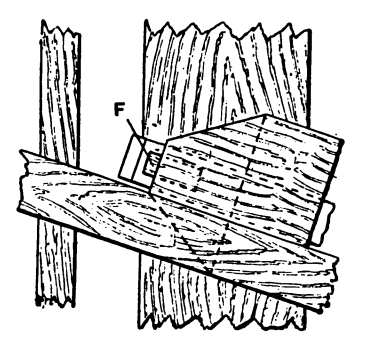
\includegraphics[width=0.6\textwidth]{Figures/_020.png}
		\caption*{Fig. 20.--Wedges and Chisel of Home-made Plough.}
	\end{figure}
encloses the chisel just below the shoulder when the
chisel is lying in the position above described.
Insert a little wedge above the chisel beneath G
(Fig. 19) so that the blade is prevented from moving
up and down; also put in wedges at D and E, and
one above the chisel at F (see Fig. 20). The whole
will then be perfectly rigid, and the chisel will be
firmly fixed in position, though, by taking out the
wedges, it can be withdrawn readily for the purpose
of sharpening it. Being thus easily removable, it
is as useful as ever for other purposes than cutting book edges.

The body of the plough is now complete. It is,
\pagebreak
of course, intended to be pushed to and fro upon
the right cheek of the press; but the tool, as it
stands, will not cut straight through so as to leave
a nice flat surface, but will rise until it has made
a "hog's-back."  To prevent this, provide a bar of
wood H (Figs. 18 and 19), which should be fixed at
one end to the top G of the plough, and should rest
at the other end on a guide-rail J fixed to the top
face of the left cheek of the press. The bar should
be rigid, say of 1/2-in. stuff about 8 in. long, and be
fixed to the plough with two screws. The top surface
of the rail must be level with the top face of B
(see Fig. 18); the easiest way to effect this will be
to make the rail J of the same stuff as Fig. 17, and
let it stand at each end on feet L (Fig. 18), made of
the same stuff as Fig. 16. The bar will then lie
quite horizontal across the press. Notice, too, that
the rail J should be set back 1 in. or more from the
inner edge of the left cheek, otherwise it will
interfere with the "backing" operations.

In working, grasp the body of the plough with
the right hand, and with the left keep the end K
(Figs. 18 and 19) of the bar always touching the
rail. When it is desired to work the plough outwards,
set the detached end of bar K a little outwards
so that the bar shall be at a slight angle, as
shown in Fig. 19. Keep it at that angle, and move
the plough from the near end of the book to the
farther end, pressing the chisel edge quite lightly
against the book. The first finger of the left hand,
as it presses against the side of the rail, will
regulate to a great extent the depth of the cut. If the
woodwork has been properly executed, it will be
possible to work the plough both backwards and forwards
by simply alternating the left end of the bar;
but if there is any unevenness in the woodwork, the
chisel edge will not travel both ways in identically
the same line, but will make two separate cuts. In
such a case the plough must be worked one way
\pagebreak
only--it will not matter which. The edge of the
chisel, as used in this case, should act with a drawing
cut like that of a knife, and not with a thrusting
cut like that of a chisel as ordinarily used. Be
careful, therefore, not to incline the bar more than is
shown in the illustration.

It is of the greatest importance that the chisel
edge should be kept very sharp and in good shape
by means of grindstone and oilstone. It is also
important that the book edges be screwed up tight
in the press. If the press used is an amateur
contrivance of 1-in. stuff worked with screw bolts, as
shown by Figs. 18 and 19, fix a little platform for
the plough to run along upon the top of the right
press cheek, and support the rail on brackets M
	\begin{figure}[h]
		\centering
		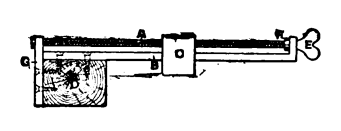
\includegraphics[width=0.6\textwidth]{Figures/_021.png}
		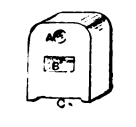
\includegraphics[width=0.25\textwidth]{Figures/_022.png}
		\caption*{Figs. 21.--Plough.  Fig 22.--Sliding Block for Plough.}
	\end{figure}
fixed to the outer side of the left cheek. A cutting
board of some sort (not shown) must be placed
against the left side of the book.

The plough shown by Fig. 21 is for use with the
lying press shown by Fig. 13, p. 18. It has a screw A
made by threading from one end to the other a piece
of iron wire about No. 4 B.W.G., 8 in. long. Fix a
washer at F with a bit of solder, leaving enough of
the wire projecting beyond it to pass through the
hole in the flat bar and for a thumb-bolt E to screw
on. The wing-nut can be made of brass, with a
rounded neck and flat wings. Drill and tap it to
screw tightly on to the wire, and leave it before
fixing it on while the bar B is made. Procure
8 in. of 1/4-in. by 1/2-in. flat iron, and bend about 3/4-in.
up at one end, as shown in the sketch. File it up
\pagebreak
perfectly true and smooth all over, and then drill
a hole at F for the screw to pass through easily,
and drill and countersink two holes at the other end
for the heads of two 1-1/2-in. screws to drop in. C
(Fig. 21) is the sliding block, and D is an end view
of the runner block. It is important that the sliding
block (Fig. 22, p. 25) be accurate. Get a block of
brass 1 in. by 1 in. by 1-1/4 in., carefully square it up,
and then round the top corners a little, as illustrated.
Cut an oblong hole 1/2 in. by 1/4 in. at B for
the bar B (Fig. 21) to pass through. If two holes
(not quite 1/4 in. in diameter) are drilled through side
by side, it will be easy, with a small chisel and file,
to cut the hole to the desired shape. See that it fits
the bar well--not loosely--and then drill and tap
a hole at A the same size as the screw already made.
If the block is slid along the bar till it is against
the bit that is turned up, the proper position for
the hole will at once be found by passing a needle
through the hole already in the bar and marking a
corresponding circle on the block C. If any doubt
exists about getting these holes through accurately,
mark the block on both sides, and drill also from
both sides till the holes meet in the middle. Next
cut the slot C 1/16 in. deep and 3/4 in. wide, dovetailed
to fit the bar B. Bevel a bit of good steel, 3/4 in.
broad and 1/16 in. thick, to fit in the block tightly,
and, while it is in, drill and tap a hole through it,
and also into the block, so that a small screw may
be inserted to keep it from slipping out when it
is in use. Make a small screw for the purpose just
stated, and then proceed to finish the knife (Fig. 23).
Be careful, when the screw is put into its place,
that it does not project above the surface of the
knife, or it will tear the edges of the book as it
passes to and fro when in use. The knife is now
rounded at the end, as seen in Fig. 23, and then
bevelled off to the shape shown. Fig. 23 represents
it as it would appear if looked at from underneath.
\pagebreak
When it has been nicely tempered, it may be fixed
in its place in the block. A piece of flat iron, 2-1/4 in.
long and about 1/2 in. broad, forms a support for
the end of the long screw. This is shown at G
(Fig. 21 ). Near the top drill a hole in which the
screw A revolves, and make two holes for the screws
which fix it in its place, and the various parts of
the cutter are ready to be put together. Slide the
block C on to the bar B and the long screw A, and
fix the wing-nut on the end by screwing it on
tightly, and then secure it by passing a small screw
through the neck into the screw A. Now fix the
	\begin{figure}[h]
		\centering
		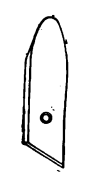
\includegraphics[width=0.2\textwidth]{Figures/_023.png}
		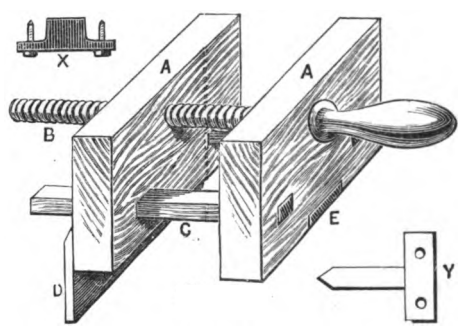
\includegraphics[width=0.7\textwidth]{Figures/_024.png}
		\caption*{Fig. 23.--Plough Knife.  Fig. 24.--Plough.}
	\end{figure}
bar on a piece of 2-in. by 1-1/2-in. wood about 8 in.
long and screw on the guide-plate G. It will be
advisable to fix on two pieces of metal, as in Fig.
13 (p. 18), to keep the cutter from twisting. This
tool will cut through any book as perfectly as one
costing a hundred times as much.

Still another kind of plough, resembling one
previously described, however, is illustrated by Fig.
24. To make it, obtain two pieces of seasoned beech
for the sides A, about 8 in. long by 4 in. deep, and
1-1/4 in. or 1-1/2 in. thick; also obtain a 3/4-in. iron
screw and nut with tail, to insert in the side
\pagebreak
opposite to the handle. By using a wooden screw,
a hole could be tapped in the side piece, and the
trouble of inserting the iron nut would be saved.
Two guides C, say 10 inches long and 1 in. square,
are fixed in the handle side, say 1-1/2 in. from the
bottom: they slide through square holes. A notch
is made to receive the cutting knife, as shown at E,
so that when put on with two screw nails the knife
is flat with the wood, as will be seen. To ensure
movement in both directions, a hole is bored
through the screw spindle for the pin and washer.
The side now is all of one piece, and will move
out or in as required. It remains to put a slip of
wood or iron on the other side, so that it may hold
on to the press bar B while working the plough
backwards and forwards to cut the edge held in the
press. This hardwood slip is shown at D. X (Fig.
24) is the iron which carries the knife, the shape of
which is indicated by Y.

The guillotine is another kind of cutting machine
for trimming the edges of books. The name of the
machine sufficiently explains for the present purpose
its construction and the manner of using it. It is
expensive, and is used for cloth books.

The tub is the stand on which the lying press is
supported. The sides of the tub are often boarded
up for some distance from the floor, to contain the
shavings cut from the book edges. A large, open
rectangular packing case makes a good tub.

A pair of large stout shears (similar to those
employed by tinsmiths), one handle of which is held in
the press, the other being worked by the binder,
is desirable when much cutting up of millboards for
book covers has to be done, though a sharp knife,
like that used by shoemakers, will answer the purpose.
It is, of course, obvious that a smooth, hard
bed for cutting on must be provided, and, if a
knife is used, a steel straightedge or T-square is
required as a guide for the knife. A grindstone
\pagebreak
and oilstone are very economical additions, for all
cutting tools must be kept sharp.

The holing machine is used for perforating the
covers of books. These holes are intended for the
reception of the ends of the bands or cords by which
the book is attached to its covers; but a bradawl
or a bodkin or a small punch will answer the purpose
of a holing machine. A tenon saw is required
for making the "kerfs," which are grooves or cuts
made across the back of a book to hold the bands
or cords upon which the sheets of the book are
sewn. These cuts are made when the book is
screwed up tightly in the lying press.

Backing boards are of very hard wood, as they
have to resist considerable strain, and are made in
pairs, of the usual book sizes. The purpose for which
backing boards are used, and the shape of the boards
(the bevels being somewhat exaggerated for the sake
of clearness), will be seen on reference to Figs. 35
and 36, pp. 49 and 51. Cutting boards, as their
name implies, are placed on each side of the book
when its edges are cut, and they are not so thick
as backing boards. Though both backing boards
and cutting boards can be made by an amateur, he
is advised to purchase a pair of backing boards to
serve as a pattern for those he may afterwards make.

Sundry small tools include one or two pairs of
scissors, a sharp-pointed knife for squaring plates--
that is, single-leaf illustrations--large sewing
needles, a small wooden tub for thick paste and an
earthenware vessel for thin paste, a large glue-pot
for thin glue and a smaller pot for thick glue, with
brushes for applying both paste and glue, sprinkle
pot (any large stoneware vessel or gallipot will do),
a sprinkle-brush, which must be a well-made brush
with a stout wrought-iron ferrule (not a bit of
common hoop iron, but a ferrule made by a smith), an
agate burnisher, that known as a dog's tooth being
\pagebreak
the most useful, a backing hammer, a small round
marble slab and paring knife, one or two bent
pointed folding-sticks, and a pair of iron compasses.
Many of these tools, or such as may very well be
substituted for them, are already possessed by the
majority of amateur workers. Other tools may be
constructed, or may be purchased second-hand of
printers' brokers. An ingenious amateur will contrive
many mechanical aids for facilitating his work
as soon as he understands the purpose to be
accomplished. An expensive plant, therefore, is not
absolutely necessary to enable anyone to begin
	\begin{figure}[h]
		\centering
		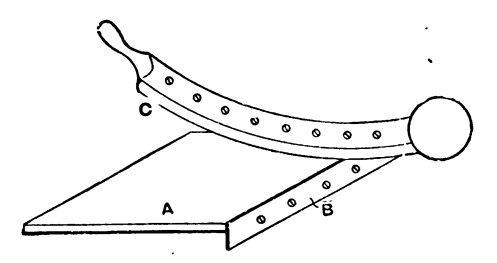
\includegraphics[width=0.8\textwidth]{Figures/_025.png}
		\caption*{Fig. 25.--Strawboard Cutter.}
	\end{figure}
bookbinding. It is, however, obvious that proper
tools and machines lessen labour and save time.

It is possible that particulars of a machine for
cutting strawboard, cardboard, etc., may be useful.
The appliance shown by Fig. 25 consists of a wood
or iron table a resting on a framework and four legs.
On the table are gauges, which can be so adjusted
that the operator can cut the boards to any size
required. Close to the edge of the table is a clamp
to hold the boards in position while being cut. This
clamp is worked by the foot, a treadle being provided
at the bottom of the legs, near the floor. The
boards are cut between two knives, one, B, being
screwed flush to the edge of the table, and the
other, C, being movable and screwed to the lever.
\pagebreak
The edges of the knives are bevelled like scissor
blades; in fact, the machine is simply a large pair
of scissors. A balance weight at the end of the
movable arm carries the knife and keeps it in position.
Both knives should be made of steel, and in
tempering them avoid getting them too hard, or
they will be liable to chip. Fig. 26 represents the
gauge A on top of the table. This gauge is simply
an L-shaped piece of metal; the shorter branch
of the L is bent to lie close to the edge of the table.
A slot almost the entire length of the gauge is cut in
the latter. A thumbscrew screws into the edge of
the table and fastens the gauge in position. The
	\begin{figure}[h]
		\centering
		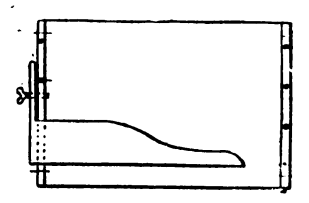
\includegraphics[width=0.6\textwidth]{Figures/_026.png}
		\caption*{Fig. 26.--Gauge of Strawboard Cutter.}
	\end{figure}
other portion of the gauge lies flat on the table. The
clamp is a light casting shaped like Fig. 27, p. 32.
It is fitted to the table close up to the knife B
(Fig. 25). A short rod is fixed at one end of the
clamp and a longer rod at the other end, ending in
a stirrup for the foot. These rods are fitted with
springs which raise the clamp and hold it up until
the foot is placed in the stirrup. A little pressure
on the stirrup brings down the clamp and holds
the board while it is being cut. The stirrup should
reach almost to the floor for convenience of working.
The side of the table and the front of the
gauge must be a perfect right angle, otherwise
difficulty will be experienced in cutting the boards.
straight. Strips of iron, not quite in. thick and
perfectly straight on the inner edges, are screwed
\pagebreak
to the top of the table as shown. The strawboard
is placed against these strips and the gauge when
	\begin{figure}[h]
		\centering
		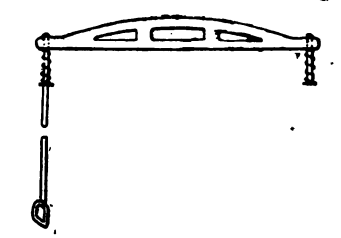
\includegraphics[width=0.6\textwidth]{Figures/_027.png}
		\caption*{Fig. 27.--Clamp of Strawboard Cutter.}
	\end{figure}
cutting, the clamp is applied, and the knife brought
down forcibly. Such a machine is in general use
amongst bookbinders, paper-box makers, etc.

Bookbinders use large quantities of glue in their
work, and doubtless much time would be saved by
employing some such preparation as "Gloophlex," an
elastic glue, guaranteed by the makers to be strong
and reliable. As bought, it has the smell and appearance
of consistent glue-jelly, and the only preparation
needed is to melt it by heating it on a water bath, and
then add boiling water according to requirements.

\vspace*{\fill}

\pagebreak

\fancyhead[CO]{\textit{FOLDING PRINTED BOOK SHEETS.}}

\thispagestyle{empty}

\vspace*{\fill}

\begin{center}

\begin{large}CHAPTER II.\end{large}

\begin{small}FOLDING PRINTED BOOK SHEETS.\end{small}

\end{center}

\noindent
The first operation in bookbinding is folding the
printed sheets, and it requires great care if the book
is to have a good appearance when bound. It is
usual for printers to leave more margin to the outsides
of the sheet, so that when the sheets have
been folded the margin will be broader at the
fore-edge and tail than at the head and back. The
head and back are always at the fold, the tail and
fore-edge being towards the outside of the sheet. If
the paper presents any little difference in size, the
two latter edges being cut first in the process of
binding, the difference will then be taken off, and
the margin will be the same all round.

The plan adopted is to fold to the pages of print,
and not to the edge of the paper, for the least
variation in the size of the sheet would result in a
spoiled book.

Papers are made in various sizes, and are known
by the following terms: Imperial (30 in. by 22 in.),
royal (25 in. by 20 in.), demy (22-1/2 in. by 17-1/2 in.),
crown (20 in. by 15 in.), foolscap (17 in. by 13-1/2 in.),
and pott (15 in. by 12 in.); and the sizes of books
are denominated according to the number of leaves
into which the sheet is folded. The ordinary sizes
are folio, 4to, 8vo, 12mo, 16mo, 24mo, and 32mo.
A sheet, when folded, has twice as many pages as
leaves, for the obvious reason that it is printed on
both sides. In speaking of the size of \textit{The Quiver},
for example, it is said to be royal octavo (8vo),
because the sheet has been folded to one-eighth its
original size, and has sixteen pages. The octavo is
\pagebreak
the most general size of a book, and the type matter
is so imposed that, when the sheet is folded, the
sixteen pages will follow consecutively.

In the early days of printing only a few pages
could be printed at one operation. Now, however,
the number of pages that can be printed on one
sheet of paper is only limited by the size of the
printing machine. But, as a matter of convenience,
the sheets the binder has to deal with usually consist
of 4, 8, 16, 32, 64, or 128 pages, the number of
pages that are folded into one sheet depending on
the price at which the book is to be sold. In the
best work, the sheets do not contain more than
sixteen pages--that is, eight pages on each side
of a sheet of paper; and each sixteen pages is
called a section or sheet. At the bottom of one of
the pages (the first numerically) of each sheet is
printed a letter or figure, known as the signature;
this is the guide when folding, and, as the letters
or figures follow each other consecutively, the
placing of the sheets in their proper order when sewing
them is thus ensured. Thus, when the sheets in a
work each consist of sixteen pages, the signatures
will be found at the foot of pp. 1, 17, 33, 49, etc.
The manner of folding is as follows: A printed sheet
(say, pp. 1 to 16) is laid on a table in front of the
operator, that side of the sheet containing p. 1 (the
signature side) lying in contact with the table.
Page 2 backs p. 1, and p. 2 should be the corner
page close to the operator's left-hand (see Fig. 28).
The corner page at the folder's right-hand is p. 3.
The object to be obtained is to fold the sheet over
in such a way as to place the figure 3 exactly on the
top of the figure 2. If this is properly done, the
printed lines on p. 3 will lie exactly on the printed
lines on p. 2, line for line, and when the book is
bound the white margins round the print on each
page will all be of the same relative widths, the
front and the bottom margins being always wider
\pagebreak
than the top and the inside margins. The result
of the first fold is shown by Fig. 29. The second
fold brings pp. 5 and 12 over on to pp. 4 and 13;
the result of this fold is shown by Fig. 30. The
third fold brings p. 9 on to p. 8, the folded sheet is
turned over, and the result seen by Fig. 31. The
first page is p. 1, containing the signature, in this
case the letter A, and the last page of the sheet is
p. 16. All folding operations follow this general
plan of doubling over the sheet for each fold; to
this rule there are, of course, a few exceptions, but
these are easily recognised. Before beginning to
fold, the folder should ascertain how many pages
	\begin{figure}[h]
		\centering
		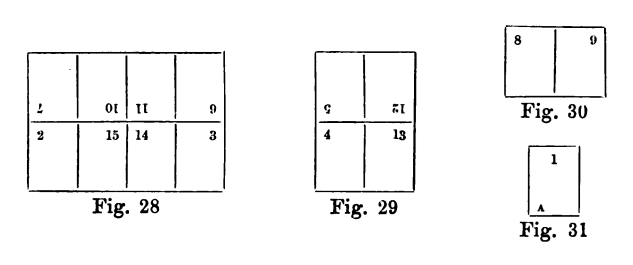
\includegraphics[width=\textwidth]{Figures/_028-031.png}
		\caption*{
			Fig. 28.--Printed Book Sheet.
			Fig. 29.--Printed Sheet, First Fold.
			Fig. 30.--Printed Sheet, Second Fold.
			Fig. 31.--Printed Sheet, Third Fold.
		}
	\end{figure}
are contained in a section. To every section belongs
a distinguishing signature or letter, and all the
pages coming between the first page of, say, signature
A and the first page of signature B belong to
signature A. Thus it may happen that signature A
consists of thirty-two pages; but in order to ensure
better folding, the thirty-two pages are printed so
as to fold in two sections, one of which is inserted
in the centre of the other. The pages and signatures
are then arranged as follows: The outer sheet
contains pp. 1 (signature A) to 8 and pp. 25 to 32;
the inner sheet, called the inset, contains pp. 9
(signature A*) to 24. The sheet and its inset are
\pagebreak
folded independently of each other in the manner
already described, and when the inset is inserted
p. 9 follows p. 8, and p. 25 follows p. 24. This is
the general rule applicable to all insets of this
character. Exceptions to this rule may, of course,
occur, but these exceptions would probably be
caused by the limited plant of the printer who
produced the book. A sheet may consist of several
insets, but the signatures would follow the rule
already stated. The worker must be always on the
look-out for things of this kind. Figures as well
as letters are used as signature marks; where
letters are used, the first sheet of the book (excluding
the title and contents) sometimes begins with B
instead of A, and the letters J and V are not used in
all cases. The folder is held in the right hand, and
is used for smoothing the folds, etc. Creasing and
puckering of the folds must be guarded against;
these mishaps readily occur if the folder is not
properly used.

In order the better to describe the further stages
of binding, let it be supposed that the operator is
dealing with one book consisting of nineteen sections,
each section, except the title sheet, which
contains eight pages only, consisting of sixteen
pages. This will give a total of 288 pages of text
and eight pages of introductory matter, consisting of
title page, preface, and contents. The signatures
of the sheets, omitting the letter J, will run from
B to T, and the title sheet will not contain a
signature. The sheets must be placed in their proper
order, and the folded edges, which will be the
heads and the backs of the sections, brought level
by knocking them up on the table. The embryo
book may now be placed in the press between a
couple of boards, and subjected to pressure in order
that the sheets may lie closely together.

In large establishments, folding is done by
machinery, without which it would be impossible
\pagebreak
for the enormous quantities of work to be turned
out. There are a great many machines in the
market, and it would be difficult to say which is
best. Nearly all bookbinders' engineers manufacture
folding machines, and some are manufactured
with special features to suit certain requirements.
Cundall's is a very good machine, which does its
work well without any special attention, and will
do two, three, or four folds. It has a nice tidy
delivery, and is easily set from one size to another.
Its speed is close on 1,700 per hour, so that, with
a very ordinary feeder, it will fold 1,500 sheets per
hour. The Salmon machine acts much on the same
principle. The name of Martini is well known in
England in connection with the Martini-Henry
rifle, but on the Continent his name is still more
famous for the invention of the single and duplex
folding machine; and a wonderful machine it is,
folding sheets of paper by means of a series of
cross metal knives, folding true to register, and
delivering in a trough already knocked up. Binders
in this country were slow in adopting this class of
machine. With the tape machine there always is
a large number of re-folds at the end of the day's
work, and there is the risk of a tape breaking at an
awkward moment. Both of these evils are entirely
obviated by the Martini folders, for there is not an
inch of moving tape used to carry the sheet from
fold to fold. Two girls feed the machine; they
stand each with a pile of sheets below her hand,
at the ends of the machine, feeding them one by
one to the points or gauges. The sheet is carried
immediately to the centre of the table, first from
one side, then from the other, the knife going up
and down away from where the girls are standing,
causing the sheet to disappear. Such a machine
can get through an enormous quantity of work.

\pagebreak

\fancyhead[CO]{\textit{BEATING AND SEWING.}}

\thispagestyle{empty}

\vspace*{\fill}

\begin{center}

\begin{large}CHAPTER III.\end{large}

\begin{small}BEATING AND SEWING.\end{small}

\end{center}

\noindent
It has already been suggested (see p. 11) that
beating is now confined almost wholly to small offices,
although in special cases it may be adopted even
when a rolling machine is generally used. Beating
is, however, the cheapest process for the amateur.
The object of beating is to make the leaves of a
book lie close together, so that the volume when
bound may be as solid as though it were one single
block. Mere pressing alone will not do this. In
beating, the bookbinder stands before the beating
slab, holding in his left hand a bundle of as many
sections of the book as he deems advisable to
operate upon at once, say, from five up to ten or
fifteen, according to the thickness of the paper.
The bundle of sheets is beaten for some time with
the hammer, which has already been described. The
proper use of the beating hammer requires so
much manual dexterity that it is advisable to
practise beating with a few folded sheets of blank
paper. The handle is grasped with the right hand,
with the big knuckles downward and the wrist
curved. The wrist and hand are then slightly
twisted so as to give the face of the hammer an
upward turn that almost permits the operator to
see the face of the hammer. Then, by a downward
turn, the hammer is allowed to descend on the work.
The blow must be given with very little more force
than is furnished by the weight of the hammer.
The hammer must not by any chance fall edgewise
on the sheets; if it does, many leaves will be cut
through, and the work spoilt. The bundle of sheets
\pagebreak
must be constantly shifted and evenly struck all
over, and a sheet of stiff, smooth paper, placed at
the top and bottom of the bundle, will keep the
sheets clean. The solidity of a bound book depends
on the amount of beating or rolling it receives.
If it is necessary to bind very recently printed
sheets, they must not be beaten or rolled; nor
should this be done if the ink is so wet as to smear,
or the ink will set off, as it is technically termed;
that is, the printing on each page will be partly
transferred to the facing page, and both pages will
be somewhat illegible. The sheets of a new work
should, before they are folded, be hung on lines in
a dry, well-ventilated room till the ink is thoroughly
dry. Test the sheets by placing a piece of white
paper on a printed page; rub the paper hard with
a folder or the finger nail, and if there is then no
sign of setting off, the sheets may safely be beaten
or rolled.

Many bookbinders who possess a rolling machine
will probably roll an amateur's work at a very small
cost. There are also houses that do rolling for the
trade. Beating, however, will answer very well.
Indeed, very old books should on no account be
rolled; the paper on which they are printed being
uneven in thickness, and the actual printing having
been done under varying degrees of pressure, careful
beating must take the place of rolling, or the
work will be spoilt. After the sheets of a book
have been beaten a few at a time, all the sheets of
the volume should be beaten together and then
placed once more for a short time in the standing
press.

Cutting with a saw several kerfs or channels
across the back of the book is the next operation,
and this is to allow of sewing. In order to do this,
the book (either one or many) is screwed up in the
lying press, either between pressing boards or backing
boards, which are placed slightly below the
\pagebreak
level of the back to allow the cut to be made. If a
lying press is not available, an ordinary carpenter's
bench will answer the purpose. The back of the
book is, according to its size, now divided into a
certain number of spaces, mostly equal; but owing
to a common optical illusion, in order that all the
spaces shall appear to be of the same size, the
bottom space must be about 1/2 in. larger than the
others. At the points of division lines are drawn
across the back of the book, and these lines mark
the bands or cords on which the book is to be sewn,
through, for ornamental purposes, books are often
marked up for, say, five bands and only sewn on
three, the dummy bands being fastened on when the
book receives its cover. In flexible work the back
is not sawn in except for the kettle stitch or catching
stitch, the bands or cords being outside the sheet,
the thread being sewn around them. In the other
kind, the back is sawn across at the places marked,
the cut for the kettle stitch being very shallow,
only deep enough, in fact, to take a chain stitch of
single thread. Octavos are generally sawn for five
bands; larger or smaller books have more or fewer
bands, according to size, because in the larger
books the number of leaves in a section are few,
and the thread has less substance to hold on to
than in the smaller books.

The twine or string used for the bands varies
in size according to the size of the book; it is
named after it, and is sold by that name. In the
case of large books, where the cord is thick, a plan
that has been successfully adopted is to use two
pieces of thin cord instead of one thick piece. This
method has much to recommend it.

The cuts, which are made with a tenon saw,
should be perfectly level, should not be deeper on
one side than on the other, and should be just
large enough to receive and hide the cord. If the
saw has a thin blade, it should be inclined just a
\pagebreak
little alternately to the right and to the left, so as
to widen the bottom of the kerf. Fig. 32 shows the
saw kerfs.

Sewing books is very simple, but somewhat
	\begin{figure}[h]
		\centering
		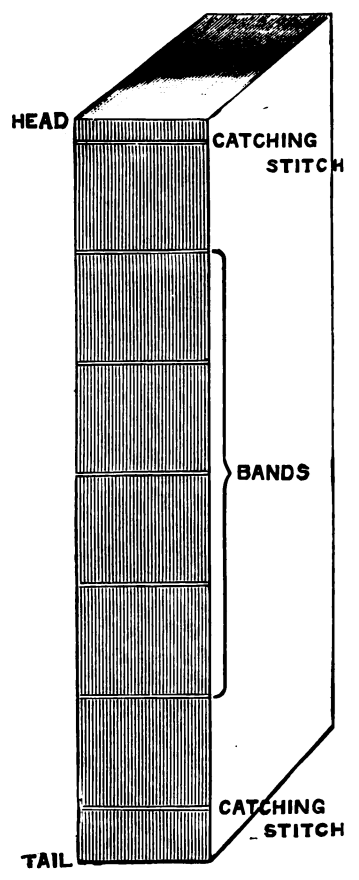
\includegraphics[height=1.1\textwidth]{Figures/_032.png}
		\caption*{Fig. 32.--Saw Kerfs in Back of Book.}
	\end{figure}
\pagebreak
difficult to describe clearly. The amateur should
endeavour to obtain some practical instruction in
the art. The sewing press and keys are illustrated
by Figs. 4 to 10, pp. 13 to 16; the other requisites
are cord for the bands, thread, needles, and a couple
of folding-sticks. The cross-bar of the press having
been screwed up to the proper height, the required
number of loops of string are fastened round
it. To each of the loops a length of cord is attached
by a bow knot that can readily be untied, and the
other end of the cord then is wound round a key,
which is pushed lengthwise through a long slot in
the front of the bed of the sewing press, and then
turned crosswise to it below, so as to remain in that
position. The bands are adjusted to correspond
with the saw kerfs in the back of the book, and the
cross-bar of the sewing press is screwed up by turning
the wooden nuts on each screw until the bands
are taut. The press is placed on the edge of a
bench of suitable height, and the sewer sits before
it in such a position that the left arm rests on the
bed of the press (see Fig. 33). Bookbinders' thread,
which must be of good quality, is supplied by the
dealers in bookbinders' materials, as are also the
needles. If only one book is to be sewn it will be
found convenient to raise it from the bed of the
press by placing another book under it. It is, of
course, a saving of time in the preparation of the
work to sew at one sitting as many books as the
press will hold. The first and the last sections of
a book should be overcast, this being generally done
with fine cotton. The sewer lifts the first section
of the book from the pile of sawn sheets on the
bench. This, which will be the title sheet (consisting
of the title page and contents), is placed
face downward on the bed of the press so that
the several cords enter their respective saw channels.
The head of the book is at the sewer's right
hand. The needle is passed into the saw cut for
\pagebreak
the kettle stitch at the tail of the book, then passed
along the middle of the section and out at the near
side of the first cord. The needle next enters on
the farther side of the cord, passes along the middle
of the section to the centre cord, and out on the
near side. The needle again enters on the farther
side of this cord, passes along the middle of the
section to the third or top band, and is brought out
on the near side. The needle is then inserted on
	\begin{figure}[h]
		\centering
		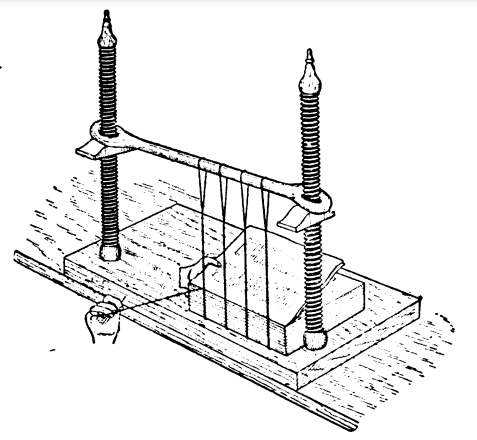
\includegraphics[width=0.8\textwidth]{Figures/_033.png}
		\caption*{Fig. 33.--Sewing Book.}
	\end{figure}
the farther side of this cord, passes along the
middle of the section, and comes out at the side of
the kerf made for the top kettle stitch. The thread
now runs along the centre of the section from kettle
stitch to kettle stitch, except where the cords occur,
where it passes round the outside of them. It is
obvious that by this process the sheet is securely
attached to the bands or cords. The thread is now
drawn tight and smooth, about 1 in. of the end
being left protruding from the lower kettle stitch.
The second sheet of the book (which will be signature
\pagebreak
B if the first section had a signature, otherwise
it will be signature A) is laid face downward upon
the first sheet. The needle is inserted at the top
kettle stitch, and the sewing is done in the same
way as with the first sheet, except that the needle
travels towards instead of from the sewer. Having
brought the needle out of the opening for the lower
kettle stitch and pulled the thread tightly along
the section, the slack of the thread is firmly knotted
to the end thread left hanging from the kettle stitch,
the knot being made twice for greater security. The
remainder of the sheets will be sewn "two on,"
except the last two sheets, which are sewn on like
the first two sheets. In sewing two on, the sheet C
is laid on the two sheets already sewn, and the
thread, which has not been detached from A and B,
is passed from the tail kettle stitch of C to the first
band along the centre of the section. A folder is
then put in the middle of the section to mark the
place. Section D is then laid on C and is sewn
from the farther side of the first band to the near
side of the third one; then section C, the middle of
which is easily found by the folder, is sewn along
from the third band to the head kettle stitch, two
sections being thus secured by a single passage of
the needle from tail to head, or vice versa. These
two sheets are secured at the head or the tail by
making a kettle stitch. This is effected by passing
the needle under the section already sewn, up
through the loop thus formed by the thread, and
then upwards until the knot is drawn tight, taking
care that the stitch is kept in the saw mark cut for
it, and that it does not tear the back of the section.
When the needleful of thread is finished, it must
not be fastened off on the book, but the second
needleful must be knotted to the first so that the
book is sewn with one length of thread.

Fig. 34 may help to explain a method of sewing
"two on." A, B, and C represent the first three
\pagebreak
sheets; 1, 2, 3, 4, and 5 the saw-marks and the
position of the bands. The small letters, if taken
in alphabetical order, will show the outs and ins
of the needle. Thus in at a, A, out at b, in at c,
	\begin{figure}[h]
		\centering
		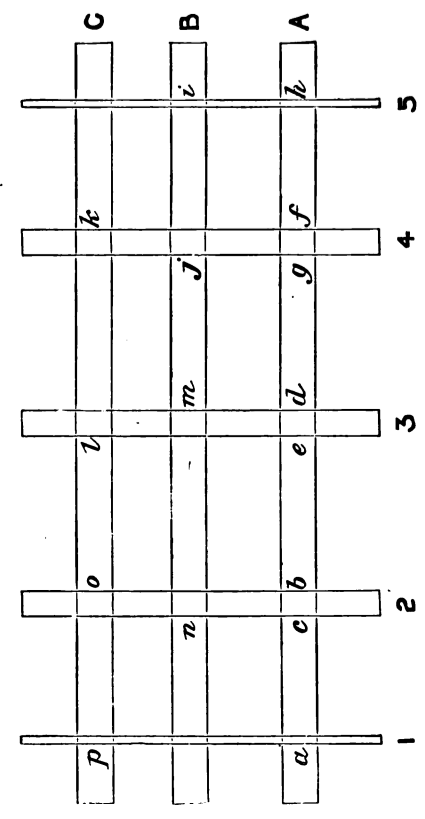
\includegraphics[width=0.5\textwidth]{Figures/_034-Rotated.png}
		\caption*{Fig. 34.--Method of Sewing Book, "Two on."}
	\end{figure}
out at d, and so on until h is reached; the needle
will be at the outside of the first sheet or A, which
will have been sewn all the way up. Now in at i,
in the second sheet or B; out at j, B; in at k, C;
\pagebreak
out at l, C; in at m, B; out at n, B; in at o, C;
out at p, C: and fasten. The diagram has little of
the appearance of a book on the bench, its purpose
being to show intricate matter plainly and
simply.

The method of sewing just described is that
which is used for non-flexible work--that is, for
books in which the back of the cover is not glued
to the backs of the sheets. In non-flexible work,
when the book is opened the back of the cover forms
an arch, leaving a space between it and the
back of the book, but in flexible work the back of
the book adheres to the cover. For flexible work
the back is marked up, but is not sawn in, the cord
or band being laid on the back of the book and not
embedded in the sheets. The marks for the kettle
stitches are sawn slightly, as in the case of
nonflexible work. In sewing, the needle is passed in
at the right-hand kettle-stitch hole; the left hand
inside the section takes the needle and thrusts it
out of the left side of the mark for the first band,
and with the right-hand the needle is taken and
thrust in on the right-hand side of the same band, so
that the band or cord is encircled with the thread.
The same operation is repeated at each band, and
the needle finally brought out at the left-hand
kettle-stitch hole. The other sheets are sewn in
the same manner.

It is hardly necessary to point out that in flexible
work the cord on which the books are sewn will,
if no corrective measures are adopted, be seen
through the leather covering. When it is desirable
that the cords should not be seen, the spaces
between the cords are levelled up with paper so that
the back presents a smooth appearance. The
levelling up is much easier when the sewing is done
with strong tape instead of cord.

When several books of the same size are to be
bound, they are usually sewn in the one stack. The
cords, which are kept sufficiently long for the
purpose, are then drawn out between the volumes and
cut off so as to leave about 1 in. of cord projecting
at each side of the back, a three-band book having
thus half a dozen ends. A few experiments in sewing
\pagebreak
will very soon demonstrate the fact that the
kettle stitches pull the head and tail of the book
together, and the thread swells out the middle.
Care must be taken, therefore, that the kettle
stitches are not pulled together too tightly, and the
swelling must be counteracted by frequently beating
down the back with a heavy folding-stick.
Attention must also be paid to the thickness of the
thread used in sewing; when the sections are thin,
the thread must be thin.

Overcasting is used when a number of single
leaves have to be bound into a book, the plan being
as follows: Having ascertained that the pages follow
each other in proper order, the book is knocked up
carefully at the head and the back and placed in
the lying press between two boards, the back projecting
about 1/8 in. above the pressing boards. The
back is roughed with a saw and sawn in, after which
thin glue is brushed over the back, and the book is
left to dry. When dry, the book is pulled apart
in sections, each section consisting of eight or
sixteen pages, according to the size and other
characteristics of the work. Each section is then
oversewn along the back, the thread being fastened off
at each end--that is, at the head or foot of the page.
This is known as overcasting; after this the sections
are hammered lightly to embed the thread. This
operation must be performed carefully, or the thread
will be cut. Then these sections are sewn in the
ordinary way, like other books. The first and the
last two sheets of a book generally are overcast to
lessen the possibility of their being torn away, by
the weight of the covers, from the other sheets.

\vspace*{\fill}

\pagebreak

\fancyhead[CO]{\textit{ROUNDING, BACKING, AND COVER CUTTING.}}

\thispagestyle{empty}

\vspace*{\fill}

\begin{center}

\begin{large}CHAPTER IV.\end{large}

\begin{small}ROUNDING, BACKING, AND COVER CUTTING.\end{small}

\end{center}

\noindent
At the beginning and end of almost any book is a leaf
of plain or plain and coloured paper popularly known
as fly-leaves, but by the bookbinders called end
papers. These end papers generally consist of a
couple of stout leaves of coloured paper, one of
which is pasted down to the cover of the book, and
the other is a loose or fly-leaf; there may also be
another fly-leaf of white paper. End papers are
made by pasting sheets of white and coloured paper
together. The coloured paper, which is specially
made for this purpose, may be purchased with other
bookbinding materials. The colour of the end
paper is governed by the binding and by the colour
of the edges of the book. The ends of the bands on
which the book is sewn should be untwisted to
separate the fibres by the aid of a bodkin and dull
knife; an end paper is then affixed to each side of
the book by pasting the back for a short way in.
When the end papers are dry, the books should be
knocked up perfectly square at the head and back
by striking them on the cheek of the lying press,
the backs being lightly but completely glued
over. The glue should not be too thick, and the
brush should be worked well in between the sections.
The glue should then be allowed to set.

In the process of rounding the binder takes a
book on which the glue has set, but is still plastic,
and gently tapping each side of the back alternately
with the backing hammer, aided by a drawing movement
of the fingers of his left hand, which holds
the book, upon the upper end paper, and a pressure
\pagebreak
of his left thumb against the centre of the fore
edge, the binder deftly gives a slight regular
curvature to the back. It is upon this curvature of the
back that the beauty of a well-bound book depends.
For example, it is the convexity of the back that
causes the agreeable concavity of the fore edge, and
adds much to the effect ofthe finishing or gilded
ornamentation of the volume.

Backing is the next operation, and is intended
to render the rounding of the back more regular,
and generally to consolidate it. The book, with a
backing board on each side, is placed in the lying
	\begin{figure}[h]
		\centering
		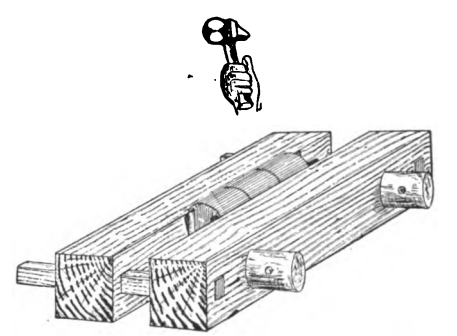
\includegraphics[width=0.7\textwidth]{Figures/_035.png}
		\caption*{Fig. 35.--Method of Backing Book.}
	\end{figure}
press, the highest part of the thick edge of the
board being within a short distance of the folded
edge of the end paper, just enough space being left
to form the joint or groove in which the board of
the cover works. The size of this groove depends
on the thickness of the cover board, which is, of
course, governed by the size of the book. The book,
with its boards, is carefully lowered into the press,
level with the upper surface of the cheeks, and
screwed up tightly. The book is then struck along
the back in order to spread it, and afterwards
carefully hammered up and down each side with the
\pagebreak
pene or face of the hammer (see Fig. 35) until the
back has become solid, smooth, and well curved;
it must also overhang the backing boards so as to
form a well-defined groove on each side for the
reception of the cover boards. At this stage of the
operations the book should present in section the
appearance shown in Fig. 36, where, however, for
clearness, the grooves are somewhat exaggerated.

Cutting the boards or side covers of the book is
the next step. The early bookbinders used wood
for the side covers of their books, and the name
has survived, though the material has changed.
These wooden covers were often elaborately carved,
and many specimens are still in existence. Deer's
hide, silk, velvet, and, later on, leather, were
afterwards used to cover up the wood. The material
employed for ordinary leather binding at the present
day is millboard.

The better qualities of millboard are made of
sound old rope or cordage, and the boards are
manufactured of different thicknesses, and are very
tough. The darker the colour of the boards the
better is the quality. Cheap millboards are
adulterated with clay, which gives substance and weight
to the boards, but does not impart tenacity.
Millboards improve by keeping, and should not be used
fresh from the mill. They are made in a variety of
sizes and thicknesses, much in the way that printing
papers are. What is termed "tip" is the thinnest
variety, and is scarcely thicker than stout brown
paper. This kind is useful for flexible bindings.
The largest and stoutest millboards are principally
employed by the portmanteau makers.

Strawboards are largely used for cheap work.
As their name implies, they are made of straw, are
very smooth and compact, but are so extremely
brittle as to be useless for any purpose but cloth
binding, cheap Bibles, and other common work. The
amateur should not use them. The covers can be
\pagebreak
set out with the compasses, and marked off with a
bodkin on a sheet of millboard of suitable thickness,
and cut up into boards of the proper size, either
with the millboard shears or with a sharp knife and
straightedge.

For the better class of leather work, the required
thickness of millboards is frequently made up by
pasting two boards together, the inside board being
thinner than the outer one. These made boards
warp a little inwards, and this ensures a shapely
cover that clings closely to the book. Single- board
covers are, with the same purpose of slightly warping
them, lined with paper. Lining should never
be omitted. Unless the boards can be cut with
shears or knife true and square at the edges, the
	\begin{figure}[h]
		\centering
		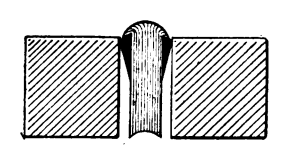
\includegraphics[width=0.5\textwidth]{Figures/_036.png}
		\caption*{Fig. 36.--Book and Backing Boards in Lying Press.}
	\end{figure}
boards should be cut with the plough. The amateur
will probably find it cheaper at first, at any rate,
to get his covers cut for him, and he should
keep a pair of covers by him as a pattern. The
covers of a book must be a little larger than the
book itself after its edges are cut, and the squares,
as these projecting portions of the cover are called,
must be ascertained and allowed for by measuring
with the compasses.

In lacing on or drawing in, a cut cover is placed
in the correct position on each side of the book,
and the positions of the bands are marked on it
with the bodkin. Two holes slightly inclined
towards each other for each band are made at the
marked places, one from the outside, near the edge
of the boards, and another from the inside, somewhat
\pagebreak
farther in. These holes can be made with a
bodkin, piercer, or awl, with or without the aid of a
hammer, or with the holing machine (see p. 29).
The bands, which have been previously untwisted
and fluffed out, then are pasted slightly, twirled up
to a point, passed through the holes in the boards
(those nearest the edge being taken first), and
drawn tight. The protruding ends are then cut off
tolerably close to the board and knocked down flat
with the hammer and left to dry and set. The bands
laced through the millboard are knocked down with
the backing hammer on an iron plate (termed the
knocking-down iron). The book is tapped along the
sides of the back with the backing hammer in order
to restore the proper curvature if it has been
impaired at all during lacing in.

In the process of scratching up or raking, the
books, with their backs protruding, are placed
between pressing boards and stacked up in the
standing press, which is screwed down tightly. After
lightly pasting the back of each book, a "scratcher
up" (Fig. 37) is drawn several times with some force
down the back, care being taken, however, not to
catch or break the kettle stitches or the stitches
over the bands. The backs are pasted again and
then scratched diagonally from left to right, and
then from right to left, being pasted after each
scratching, and the paste is well rubbed into the
grooves made by the scratches. It is then rubbed
off, and the backs are smoothed with an old cutting
board, and wiped clean with a wisp of paper shavings.
A light coat of glue is given to each back,
and the batch of books is left in the press for some
time, preferably all night. This operation gives
strength and firmness to the backs of the books.
Lining up gives stability and smoothness to the
back of a book, and it consists of gluing several
thicknesses of paper on to it. For the first few
thicknesses, good, smooth brown paper will do, but
\pagebreak
stout cartridge paper is best for the last layer, as
it offers a smoother surface to which to paste the
leather. The back of the book and the hold-on
back of the cover are both lined, as may be seen
on examining a leather-bound volume. Flexible
work is not lined, the leather being glued directly
to the book.

Headbands are purchased by the foot or yard at
any bookbinders' material warehouse, at prices
varying according to the depth and quality of the
band. These headbands are specially woven, and
are cut up in pieces the width of the thickness of
	\begin{figure}[h]
		\centering
		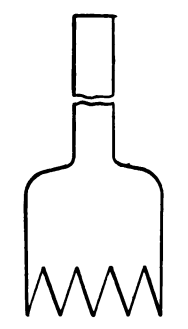
\includegraphics[width=0.3\textwidth]{Figures/_037.png}
		\caption*{Fig. 37.--Scratching-up tool.}
	\end{figure}
the book, allowing for the curve of the back, and
are glued on top and bottom, the woven pattern
coming level or flush with the edges. A reference
to any well-bound book will at once explain the
operation. Headbands are sometimes worked by
hand, silk and gold and silver thread being used.
The foundation may be of any substantial material.
The best way to learn to make a headband will be
to take an old one to pieces.

In all whole binding, and in good half morocco
or half calf, it is usual to affix raised artificial bands
to the back of the book. In the early days of
\pagebreak
book-binding, saw kerfs were not made on the back of
books, and the cords on which the sheets were sewn
formed prominent ridges across the back after the
book was covered with leather. The actual bands
are never left protruding now, except in the so-
called elastic work, but as raised bands take off the
monotony of a plain flat back and afford scope to
the finisher, artificial bands are affixed to the backs
of well-bound books, the number of bands depending
on the size of the book. For octavos, five is
a usual number. The bottom band is farther from
the tail than the top one is from the head, and this
allows for the extra fillet in finishing, which is
worked twice at the tail and only once at the head.
Bands are usually made of narrow strips of solid
stout leather carefully cut, all of one width and
thickness. The space between the bands should be
set off on the back with compasses, and the bands
securely glued on. When this has been done the
book is ready for covering.

\pagebreak

\fancyhead[CO]{\textit{CUTTING BOOK EDGES.}}

\thispagestyle{empty}

\vspace*{\fill}

\begin{center}

\begin{large}CHAPTER V.\end{large}

\begin{small}CUTTING BOOK EDGES.\end{small}

\end{center}

\noindent
Cutting the edges is performed with the plough at
the lying press. The operation is termed cutting in
boards. The plough knife should be carefully ground
and whetted, or good work cannot be done. The
head or top of the book is cut first, the back being
towards the operator. A cutting board is placed
behind the book, and a straight runner along the
millboard and level with its edge; the book is then
placed level in the press, which is screwed up
tightly. When the head has been cut, the tail or
bottom of the book is treated in a similar manner.

These operations are simple enough, but cutting
the fore edge or front of the book presents more
difficulty, as it is necessary that the curved back
should first be rendered flat. This is an operation
that requires considerable care, and if the amateur
cannot obtain a little personal instruction on this
point he is likely to spoil many books. The operator
holds the book in his left hand, permitting the
boards to fall back flat, and passes a piece of string
once or several times round the book. He then
pushes a couple of pieces of thin bevelled iron
termed trindles (see Fig. 38, p. 57) between the
book and the boards at the head and at the tail.
Taking the book between the palms of his hands,
the operator now beats the back of the book
quite flat on the cheek of the press, the cord
and trindles helping to keep the back flat.
Having made the book flat, and having marked
the front edge of the book back and front, the
operator places a cutting board level with the
\pagebreak
mark at the back of the book, and another cutting
board, or a long, straight runner, a little below the
line on the front (or right hand), and, striking out
the trindles, lowers the book into the cutting press,
the millboards hanging down. The distance below
the mark at which the runner is placed must be
equivalent to the desired square for the board at
the fore edge. When the volume is in the press, if
it has been kept level, the runner must be level
with the right-hand cheek, and the other cutting
board must stand up for the distance of the size of
the square above the left-hand cheek. When the
book is correctly fixed, the press is screwed up
tightly, and the front edge of the book is cut with
the plough as before. When the book is taken out
of the press the back will resume its convex shape,
and the fore edge should present a regular concavity.
As the cutting of the edges of the book is a very
important operation, the following points must be
remembered. The edges must be square with the
printed lines on the page, and should not be
trimmed more than is necessary. The margins of
white paper on a page must bear a certain proportion
to each other. The printer, when preparing
the pages for printing, settled the margins for the
page, and fixed also the proportions. The binder
cannot improve on this arrangement, but he can
spoil it altogether by bad cutting. The white paper
at the top of a page, measured from the type
(excluding the headline) to the edge of the paper,
and the white paper at the front of a page, measured
from the type to the edge of the paper, should be
of equal width; the white paper at the bottom of
the page, measured from the type to the edge of the
paper, should be about one-fourth more than the
front or the top margin. Thus, if the front margin
and the top margin are each 1 in., the bottom margin
should be 1-1/4 in.; the back margin in such a case
\pagebreak
would be 3/4 in., and as this margin cannot be
trimmed, the width of it compared with the other
margins shows at once whether the book has been
properly cut. It will be readily understood now
that good and accurate folding is of the greatest
importance, because the cutting of the edges of a
book magnifies any errors committed in folding.

The trained eye, however, is a better guide for
margins than the measuring tape. The book covers
	\begin{figure}[h]
		\centering
		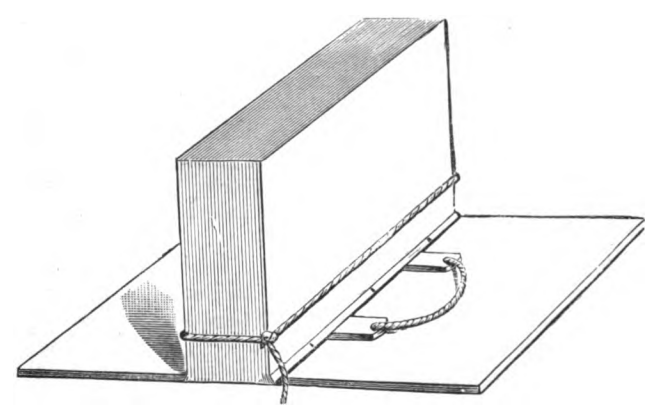
\includegraphics[width=\textwidth]{Figures/_038.png}
		\caption*{Fig. 38.--Book tied up for Cutting.}
	\end{figure}
must be absolutely square to the paper, as the paper
is to the print; the covers must not overhang the
book too much, and the amount of overhang must
be in the same proportion (the difference, of course,
is only enough to be just perceptible) as the margin
is to the printed page.

Books bound in cloth or in other cheap styles
have their edges cut on the guillotine, as the use
of the plough is too expensive for cheap repetition
work.

\pagebreak

\fancyhead[CO]{\textit{COVERING BOOKS.}}

\thispagestyle{empty}

\vspace*{\fill}

\begin{center}

\begin{large}CHAPTER VI.\end{large}

\begin{small}COVERING BOOKS.\end{small}

\end{center}

\noindent
Books may be covered either with leather or with
cloth; leather may be used either to cover the
entire book, which is termed whole binding, or a
strip of leather may be applied to the back only,
and small pieces of leather affixed to the corners,
which is termed half binding. For whole binding
the leather should be cut of sufficient size to cover
the book and to allow about an inch all round to
turn over. For half binding a strip of leather of
the desired width and rather longer than the book
should be cut for the back, and four small pieces
for the corners. The edges of the leather then must
be very carefully pared or skived, so that no
unsightly ridges can be seen. When the leather is
pasted on the covers of the book the paring is done
by laying the leather (flesh side uppermost) flat on a
marble slab or smooth piece of board, and taking
off a slanting shaving with the paring knife, which
should be very sharp.

Suppose that an octavo volume is to be bound
in whole morocco. The leather cover, properly
pared round the edges, and rather farther in at
those places that will come at the head and tail of
the back, is carefully and completely coated all over
on the flesh side with thick paste, and placed on
the work bench with the pasted side upward, and
one of the narrow edges towards the operator. The
book to be covered is taken up and the boards are
adjusted so that the squares are correct at the head
and tail. Those portions of the string bands that
have not been laced into the boards are lightly
\pagebreak
touched with thick paste; some binders also make
a practice of brushing over the back with thin glue.
The book is laid down on its side in the proper
place on the pasted cover, with the back from the
operator. The lower flap of the leather is drawn
over the upper millboard and turned in at the fore
edge; and when this is done the book is turned over
and the other side of the leather also turned in at
the fore edge. The book is then rested on its fore
edge and the leather worked tight at the back with
the fingers of both hands, as shown at Fig. 39. In
this operation the leather is not only drawn close
and tight to the back crosswise by pushing it downward
	\begin{figure}[h]
		\centering
		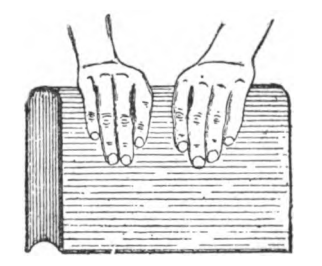
\includegraphics[width=0.5\textwidth]{Figures/_039.png}
		\caption*{Fig. 39.--Tightening Leather on Back of Book.}
	\end{figure}
on the millboards at each side of the book,
but it is also drawn tight longitudinally towards the
head and tail. The book next is laid on its side.
Each band should be raised alternately, and the
leather drawn tightly over its surface and rubbed
down with the palm of the hand or the folder till
quite level. The leather has now to be turned in
at the head and the tail. For this purpose the book
is stood on one end and the flap of leather A (Fig.
40, p. 60) turned over the end of the bands and also
over the loose fold of the paper which lines the back.
The other end of the book is treated similarly. It
now remains to turn in the corners. For this purpose
the leather is cut off diagonally to within
\pagebreak
rather less than 1/8 in. of the corner. This is bent
back from the book, a cutting-board placed under it,
and the diagonal edges are carefully pared and
afterwards pasted. The leather is accurately
doubled in level with the board at the head or tail,
as the case may be, and the part A (Fig. 41) pressed
tight to the other surface of the leather as shown.
Both the folder and the thumbnail can aid in bringing
the leather close and level. The flap of leather
B is turned over and rubbed so that it adheres to
the board. The leather above the headband at
	\begin{figure}[h]
		\centering
		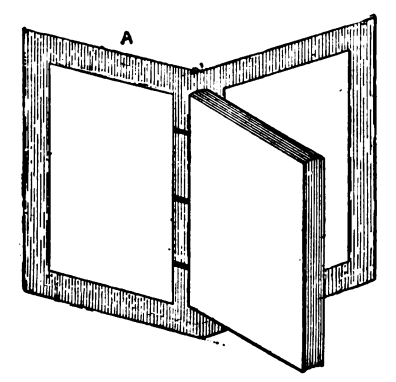
\includegraphics[width=0.6\textwidth]{Figures/_040.png}
		\caption*{Fig. 40.--Turning in Leather at Head and Tail of Book.}
	\end{figure}
both the head and tail of the book is now pulled up
a little if necessary, rubbed quite smooth with
the points of a folder, then turned down over the
headband and rubbed with the folder until it maintains
its place. This double fold of leather above
the headband is termed the cap of the headband,
and Fig. 42 shows a section through both headband
and cap. During the operation of covering, so that
thorough contact may be ensured, the leather on the
back should be well pressed and rubbed down with
the hand and the folding-stick. The edge of the
\pagebreak
folder also should be rubbed carefully on each side
of the bands to force the leather in at these angles
and make them clean and sharp. The book is then
tied up and left, generally for a night, till the
	\begin{figure}[h]
		\centering
		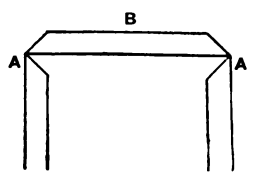
\includegraphics[width=0.4\textwidth]{Figures/_041.png}
		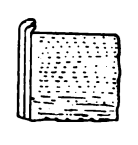
\includegraphics[width=0.2\textwidth]{Figures/_042.png}
		\caption*{
			Fig. 41.--Turning in Corners of Leather.
			Fig. 42.--Section through Headband and Cap.
		}
	\end{figure}
paste has set. Tying up is effected by first tightly
tying a loop of packthread lengthways round the
book at the joints; that is, at that part of the book
	\begin{figure}[h]
		\centering
		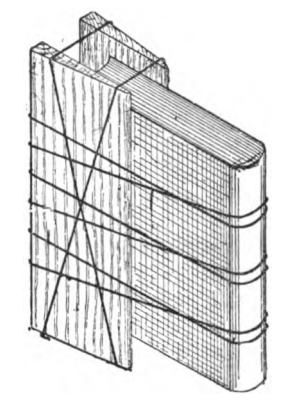
\includegraphics[width=0.35\textwidth]{Figures/_043.png}
		\caption*{Fig. 43.--Book tied up in Boards.}
	\end{figure}
where the boards are hinged to the back. A
stronger piece of twine then is wound several times
round the book, so that it passes on each side of
each band, as shown at Fig. 43. A pair of backing
or cutting boards should be tied at the fore end of
\pagebreak
the book as shown, to prevent the string marking
the leather.

Covering with calf, goat-skin, roan, or any other
leather, is conducted in the same manner. The calf
cover must be soaked in water, carefully wrung out,
and all the creases made by the wringing smoothed
out before the skin is pasted. If the book is to be
covered with white vellum or forril, the millboards
and back should be covered with clean white paper,
or the colour of the vellum will be degraded by the
colour ofthe boards underneath. Half-bound books
	\begin{figure}[h]
		\centering
		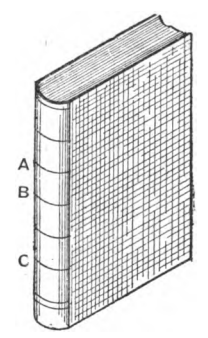
\includegraphics[width=0.3\textwidth]{Figures/_044.png}
		\caption*{Fig. 44.--Book with Square Lettering Pieces.}
	\end{figure}
are covered in the same general manner. The four
corners are first pasted and affixed, and then the back.

Books bound in morocco or roan are usually
lettered directly on the leather. But as this plan
does not answer well with calf, it is usual, when
binding in calf, to affix a small square of smooth
morocco on the back at the place where the title is
to appear, and these tablets are called lettering
pieces. They are generally scarlet, green, or purple,
and should be in contrast to the colour of the calf;
thus, a scarlet lettering piece looks well on a book
bound in dark-brown calf, a green piece on a dark
purple, and a purple or marone piece on a fawn or
\pagebreak
salmon colour. If there is but one lettering piece,
it is usually fixed in the space between the first and
second band from the head, as at A in Fig. 44. If
a second piece is required to bear the number of
the volume, it can be placed either at B or at C.
Sometimes, when there are no raised bands, a
square lettering piece is placed towards the head
of the book, and below it a small round or oval piece
of a different colour, as shown in Fig. 45. This is an
old-fashioned method which at one time was very
	\begin{figure}
		\centering
		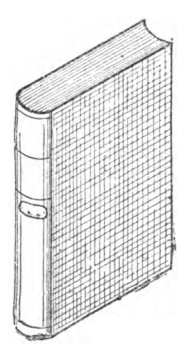
\includegraphics[width=0.3\textwidth]{Figures/_045.png}
		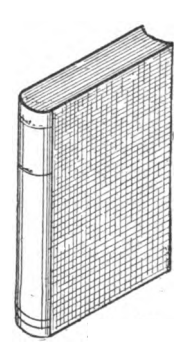
\includegraphics[width=0.3\textwidth]{Figures/_046.png}
		\caption*{
			Fig. 45.--Book with Oval Lettering Piece.
			Fig. 46.--Book with Lettering Piece at the Head.
		}
	\end{figure}
popular. For crown octavos a lettering piece towards
the head is frequently adopted, as shown in
Fig. 46, and, instead of filleting, the lower part
of the back is tooled ornamentally. The backs of the
books should be marked off for filleting before the
lettering pieces are affixed. This is done by setting
off the places of the fillet with a pair of compasses,
and then creasing or making a slight channel
at those places with the sharp edge of a thin folding-
stick, taking care that the marks shall be perfectly
straight and square across the back, as the finisher
will be guided by them in applying his fillet, roll, or
pallet across the back.
\pagebreak
Putting on sides and pasting down end papers
are two processes properly belonging to forwarding,
though the practice of different binders varies.
Some perform these operations before the books
are sent to the finishing shop; others have the
finishing executed before they affix the sides and
paste down the end papers; and some defer burnishing
the edges until after the finishing of the book.

These variations in practice are matters of convenience.
The sides of the half-bound volume may be either of
marbled paper or of cloth. If the book has
marbled end papers and edges, the sides should, of
course, match them. Cloth sides are more durable
than paper, and are much used for books that are
likely to undergo hard service. Whether the cloth
sides should match the leather back or contrast
with it is a matter of taste. In cutting the cloth
or paper the sides are cut perfectly straight along
the back, and obliquely off for the corners, as at
Fig. 47, the latter portions being so cut as to leave
the leather corners showing beyond the sides all of
exactly the same size. It is advisable to do all the
cutting with a sharp-pointed knife and pair of
cutting boards instead of scissors. Cloth sides are
affixed with thin glue, and marbled paper sides with
thin paste. The sides should be carefully rubbed
down to exclude air bubbles, and turned over, and
the edges made flat and square by rubbing with
the folding-stick. Before pasting down the end
papers, the least possible shaving should be cut
off at the head, tail, and fore edge of the leaf;
otherwise, as the leaf will certainly stretch a little
when it is pasted and rubbed down, the pasted-down
end paper might show slightly on the square of the
board, which would be an imperfection in good
binding. The end papers are then covered with
thin paste, and are carefully rubbed down to get rid
of any blisters or air bubbles. The end of the
\pagebreak
folder may be used to press home the paper at the
joints; if the end paper does not stick to the edge
of the board line, a hollow space, known technically
as a "pencil case," will be left, and this is
considered very objectionable. The books, with the
boards or covers open, should be set up on their
	\begin{figure}[h]
		\centering
		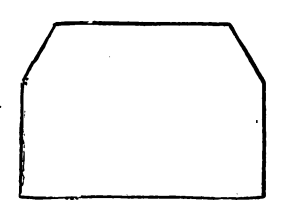
\includegraphics[width=0.5\textwidth]{Figures/_047.png}
		\caption*{Fig. 47.--Side of Cover of Half-bound Book.}
	\end{figure}
heads or tails on a bench until dry, when they should
be placed between pressing boards in the standing
press and considerable pressure applied. The books
then are ready for the finisher. Gilt-edge books
must be protected by covering their edges with
paper.

\vspace*{\fill}

\pagebreak

\fancyhead[CO]{\textit{CLOTH-BOUND BOOKS, PAMPHLETS, ETC.}}

\thispagestyle{empty}

\vspace*{\fill}

\begin{center}

\begin{large}CHAPTER VII.\end{large}

\begin{small}CLOTH-BOUND BOOKS, PAMPHLETS, ETC.\end{small}

\end{center}

\noindent
What in professional bookbinding is termed cloth
boarding is, as has already been stated, different
altogether from leather binding, but in cases where
cloth is merely substituted for leather, the earlier
steps of forwarding are the same as for half-bound
books. The edges may be left white, or sprinkled,
or gilt; it is merely a question of cost. The cloth
cover is carefully cut out to size, glued over, the
book laid on it, and the cloth drawn on, just as with
leather coverings, pains being taken to secure
adhesion everywhere and not to leave blisters. The
corners are cut off and turned in as described
for the morocco cover. The principal thing to be
attended to in cloth work is the state of the glue
and the manner of its application. The glue should
be very thin and very well frothed, so that it may be
applied to the cloth in such a state as to be readily
and equally distributed over the surface, with no
lumps and no thick or thin streaks. Cloth work
is not head-banded, but a fold of the cover at the
head and tail is turned in over the fold of the paper
lining the back. Sometimes leather lettering pieces
are placed on the back of cloth books, but this is
rarely done, and generally all lettering, filleting, and
other gilding is performed directly on the cloth.

Cloth boarding is the binding adopted for cheap
new books, and those who practice it are known as
publishers' binders. Many of the processes are
nearly identical with those used in leather binding,
but the work generally is fragile, and has little
durability, being executed very quickly and cheaply.
\pagebreak
Much of the work is done by machines, the folding
being performed at the rate of from 1,000 to 3,000
sheets per hour, according to the character of the
work. Gathering is also done with great rapidity
by a machine like a revolving table, at which
gatherers sit, and as the table revolves each
gatherer takes a sheet from the pile as it passes.
In gathering by hand, the piles of folded sheets
in the order of signatures are laid out on a long
table, and the gatherer passes along the table,
taking a sheet from each pile until a book is made
up. After collating (that is, examining each completed
book to see that the sheets have been placed
in their proper order), the books are slightly rolled
to compress the folds. Cloth books are sewn in
several different ways. If sewn on cord, the kerfs
are cut with rapidly revolving circular saws, which
make all the kerfs simultaneously. But it is more
usual now to sew this kind of work on tapes which
do not require any saw kerfs. The sewing is performed
by women at the sewing press as before described.

Books are also sewn by a specially contrived
sewing machine in which a wire thread is
employed. Such sewing can be used for ephemeral
publications, for which, and for pamphlets and
periodicals, it is admirably adapted, but it is not
recommended for leather work.

The edges of the books next are cut with the
guillotine machine. The backs then receive a coat
of glue, and when this is sufficiently dry, the books
are rounded and backed, and then lined on the
backs with a double thickness of paper.

In preparing the cloth covers or cases the millboards,
the cloth, and the stiffeners are cut to the
proper size, large quantities being done at one time.
The stiffeners are slips of stoutish paper of the
length and breadth of the back of the book. The
cloth is glued all over, the millboard laid on it,
and the stiffeners are placed between them in proper
\pagebreak
position, so as to leave a slight space between its
edges and those of the millboard, so that the case
will fit well at the joints. The cloth is now rubbed
well down on the millboards and stiffener, turned
over at all the edges, and the corners are cut off
and turned in also. These cases are finished at one
operation at the arming press. The lettering and
any ornament either for the back or sides of the
case, whether gilt or blind, is attached to the platen
of the press, which is heated by gas, and can be
brought down forcibly by working the handle, somewhat
after the manner of a hand printing-press (see Fig.
101, p. 135).

In the forwarding shop the back of the book is
glued to the back of the case, and the end papers
are pasted down to the boards. The books are then
put in the press for a time, and when dry are ready
for the bookseller's shop.

Books that are illustrated with plates independently
of the text usually contain for the guidance
of the binder directions for the placing of these
plates, and it is of course a simple matter to follow
the instructions. It must, however, first be
ascertained that the margin is perfectly square and
straight, and any error should be rectified by
cutting with a sharp knife and straightedge. In the
case of an upright picture (that is, when the
inscription reads across the bottom of the page) there
is diversity of practice in placing it in the book, some
contending that it should occupy either the right-
hand or the left-hand page, as the case may be, so
as to face the descriptive text. Many publishers,
however, insist that in all separately printed plates
the picture when the book is open should be on the
left-hand page; and this contention is, for artistic
and other reasons, undoubtedly correct. In the
case of longway pictures (that is, when the
inscription reads along the side of the page), there is
no diversity of opinion as to which is the correct
\pagebreak
position of the picture. It should always be on the
lefthand page, the inscription should always read from
the bottom to the top of the page, and should
always be on the inner and never on the outer
margin. Cases are, of course, often occurring
where both printers and binders flagrantly
disregard this arrangement, but the best authorities
never permit a longways picture to be on a righthand
page. The plate is pasted along the edge and placed
in the position it is to occupy. The visible
margins on the plate should bear the same proportion
to each other as the margins of the page.
Double plates and maps must be folded correctly,
special care being taken to see that the folds do not
appear beyond the edges of the book. In some
cases a guard is pasted at the fold, and in other
cases the ends are pasted like single plates. The
guard is preferably of stout drawing or cartridge
paper, about 1 in. or 1-1/2 in. wide; tape or narrow
linen is sometimes used. This is pasted to the
section, and permits the map or double plate to
open well when the book is opened.

Coloured plates, unless thoroughly dry, are very
liable to stick to the protecting tissue paper
generally inserted. If the plates show any disposition
to stick they may be lightly dusted over with French
chalk.

A binder is sometimes required to interleave a
book with writing paper, the object being to give a
page of white paper facing each page of print, in
order, perhaps, to facilitate the making of corrections
when a new edition of a book is required, or
there may be other reasons. The edges (top and
front) of the sheets are cut through with a knife by
hand, and the writing paper having been cut and
folded to the proper size, a four-page section of
white paper is inserted between each four pages of
printed paper. The sheets are then dealt with in
the usual manner.

\pagebreak

As regards law books, generally these are bound
in a manner peculiar to themselves. The edges are
left white as cut, and the books are whole or half-
bound in calf of the natural colour (a kind of
fawn-coloured drab). They have generally marone-
coloured or scarlet lettering pieces, and no other
ornament but a plain fillet. If in half calf, the
sides are usually of cloth, as such books have
frequently to undergo hard wear.

Pamphlet binding may here receive attention.
After pamphlets have been stitched, whether with
wire or thread, the next operation is that of
covering, if this is required. There are many ways of
covering pamphlets, and of them the following is
very economical of time--a very important item in
a long job. Supposing the pamphlet to contain
16 pp. or 20 pp., proceed thus: Lay the covers out
on the table with the inside uppermost and the
head at the right hand, knock up a parcel of, say,
twenty or fifty pamphlets, and paste or glue the
backs. Paste should be used if there is time to let
it dry. Set them down at the right hand, and lift
one and place it down in the centre of the cover and
draw the front over it. Repeat the operation
throughout the job. The operator thus will be able
to watch whether the covers are being drawn on
straight. The front of the cover has generally
more printing on it, and if there are any lines they
can be kept even, and the pamphlets will have a
good appearance when they are cut. If the pamphlets
contain a number of pages and have been sewn,
it will be best to knock them well down with the
hammer before cutting them, or they will cause
much trouble in the cutting. They should be well
rubbed in the back with the folder, to make the
covers stick properly. Pamphlets of many sections
may be stitched with thread through the side, but
it will be necessary to make holes for the needle to
pass through. This may be done with the hammer
\pagebreak
and bradawl, or a stabbing machine may be had for
the purpose. Make the first hole in the centre of
the back, about midway between the printed matter
and the outside margin, the other two at equal
distances from the first and the head and tail of the
book. However, wiring with machines has superseded
this old method. After the pamphlets have been
covered and properly dried, it only remains to
cut their edges.

The rebinding of a book requires considerable
care and circumspection, whether the book has been
already bound in leather or merely cloth-boarded.
The book must be very carefully taken to pieces,
bands and thread being cut, and the sheets gently
pulled apart, the glue being moistened if necessary.
Even if the book has been badly folded in the first
instance it is seldom advisable to refold the sheets
unless such a measure is unavoidable. In this the
binder must use his discretion. Narrow and
irregular margins and crooked pages are evils, but
it is quite possible to make matters worse by rashly
undertaking to refold such a book. Torn leaves,
often met in old books, must be carefully mended,
and any missing portions of a leaf or margin should
be replaced with small strips of paper carefully
pasted on. Paper discoloured by age should be
matched as near as possible. A perfectly clear
gum should be employed for mending, or the thin
transparent gummed paper that is sold for mending
music may be used sometimes with advantage.

\pagebreak

\fancyhead[CO]{\textit{ACCOUNT BOOKS, LEDGERS, ETC.}}

\vspace*{\fill}

\begin{center}

\begin{large}CHAPTER VIII.\end{large}

\begin{small}ACCOUNT BOOKS, LEDGERS, ETC.\end{small}

\end{center}

\noindent
Ledger and account bookbinding is a class of work
that is hardly likely to be offered to or attempted
by the amateur. Although, in a general way, the
method of binding ledgers is much like that used
for ordinary books, there are considerable differences
in matters of detail. Strength and durability
being of vital importance in a ledger, great
attention is paid to the sewing, which must be very
strong. Ledgers are not sewn on cords, but on
strips of parchment; therefore, saw kerfs are not
required. The needle is inserted at the kettle
stitch, brought out on the farther side of the band,
then back across the band, entered again on the
near side, passed up the centre of the section to
the top of the next band, and the operation already
described in the case of the first band is repeated.
The covers are made by pasting together thin millboard,
which is then subjected to considerable
pressure. Two of the boards are pasted for half
their width only, and in the opening thus left are
inserted the bands on which the ledger is sewn, as
well as the strips of canvas or leather glued across
the back. This half of the covers is then pasted,
and the book with its covers is pressed till dry.
Ledgers are generally furnished with spring backs.
The back is usually made of thin millboard, which
is warmed at the fire and worked to the shape of
the back, and then glued on. For large ledgers,
several layers of millboard are glued together, each
successive layer being a trifle smaller than that to
which it is glued. Other differences, such as
\pagebreak
leather joints to strengthen the covers, etc., will be
better understood by comparing a bound book with
a ledger.

Account-book binding--or, more properly speaking,
stationery binding--includes everything from
the penny memorandum book to the massive ledger.
Passing over the cheaper kinds of stationery, a
detailed description will be given of what is
considered to be the best and most workmanlike
method of binding an account book. After the
paper has been ruled, it is folded into sections and
prepared for sewing. If the paper is what is termed
hand-made, there will be two shades on every
sheet: one side will appear blue, and the other
white; so to prevent a blue and white appearing
together when the book is opened, the paper is
"faced, " that is, two blue sides are made to face
each other, then two white sides, and so on through
the entire book. The ruler will have left four sheets
unruled; these are for the end papers.
The joints of account-books may be of cloth,
linen, or leather. Black glazed linen makes a good
joint for general purposes. The joint is glued, and
two sheets of the four already mentioned are laid
upon the joint, about 1/8 in. apart from each other.
The other two sheets are treated in a similar
manner. Four pieces of marble paper are cut to the
size, glued all over, and laid on to the edge of the
linen and rubbed down with the hand (nipping the
papers in the press is superfluous), and hung up to
dry. Meanwhile the folding of the paper has been
going on, and it will be done up in three or four
sheet sections, according to the make or thickness
of the paper. If the sections are too thick, the
leaves will start when the book is being rounded,
and if they are too thin, in sewing the back will
swell, owing to the quantity of thread used. The
first and last section should be lined on the outside
with a strip of white calico. Some binders line
\pagebreak
the inside and outside of each section with calico;
this may be necessary in special cases, but for
general purposes it is not to be recommended, as a
book thus treated will be very stiff to open.
Account books are sewn on tapes; therefore saw
kerfs are not required. For the class of work under
notice a good strong twilled linen tape (known as
"binding") of a grey colour, and sold in rounds,
will be needed. Three or five bands, according to
the size of the book, should be set up on the bench.
Strips of vellum are sometimes used as bands in
conjunction with the tape for heavy books. To set
up strips of vellum on the bench stitch a piece of
waste tape to each end of the vellum, lap the one
end round the rail at the bottom of the bench and
the other round the cross-bar at the top, and put a
pin or a broken needle through it.

The thread must be well selected. A good linen
thread 3-cord No. 18 is a very serviceable size. Wax
the thread to preserve it and to make it wear better.
Each section of the book must be sewn all the way
up, and the needle must be brought out at the far
side of the band, and introduced again at the near
side, thus bringing the thread round the bands.
The end papers will also have to be sewn to the
book, and treated in the same manner as a section
of the book. The slips, when the book is sewn,
should project about 1-1/2 in. on each side of the
back.

Gluing up the book, the work of the forwarder,
is the next operation. The glue should be of good
quality and thin, and tolerably hot when applied.
It must be rubbed well into the sections. If the
brush does not accomplish this satisfactorily, the
thumb should be used for the purpose. When the
glue is dry, the fore-edge should be cut, and if the
edges are to be mottled instead of marbled, do the
fore-edge at this point. For instructions on this
part of the work see Chapter V. The book will
\pagebreak
now be ready for rounding. A greater degree of
roundness should be given to it than to a
letterpress book. The inside sheet of the end papers
will require to be glued to the first and last leaf of
the book. This should be done after rounding the
back, and the book put in the standing press between
tins. This pressing of books with tins should
always be done, especially in the case of account
books, as a greater degree of solidity will thus be
imparted. If the book can be left in the press
overnight, so much the better.

In the morning, as soon as the glue is ready,
get the book out of the press and line the back.
Scraps or waste pieces of strong leather are kept for
this purpose. The linings are cut to fit between the
bands and the head and tail of the book. They
should be long enough to extend from 2 in. to 3 in.
on each side of the book. Glue the linings and the
back of the book, and when attaching the lining,
rub it well down with the folder to ensure it
adhering well. The book should be screwed up in the
lying press during this operation. In lining very
heavy books, cover the entire back, the bands as
well.

Before making the back of an account book, it
will be necessary to measure for it with a strip of
paper. For this purpose, lay the paper strip on the
side of the book about 3/8 in. from the back, bring it
over the back, carry it to 3/8 in. on the other side,
and cut off. With this strip of paper for a guide,
cut three strips of good hard millboard, a special
thin but hard board for this purpose being known
as "black board." The first strip must be cut
exactly to the size of the paper; the second one a
trifle wider than the first; and the third one wider
still. These strips will of course be about 2 in.
longer than the book. Then with strong glue fasten
the strips of board together. Glue the smallest
first and each larger piece in succession so that the
\pagebreak
exposed edges of each larger piece are kept clean
and free from glue; press firmly and leave till dry.
The back must now be rolled, a wooden roller
covered with stout brown paper being necessary.
The paper is glued at one end and fastened to the
roller. Heat the back thoroughly over a gas flame
or a bundle of lighted shavings, and allow the heat
to penetrate the boards, taking care to prevent
burning. When the back is hot and pliable, place
it in the roller and give one sharp turn; then
reverse quickly and give another turn. It may
require to be reversed several times to keep all the
parts in place during rolling. Now roll up tightly,
and with a flat board, such as a backing board, roll
the back over the bench several times, pressing
heavily all the time; then set it aside to dry. The
diameter of the roller should be about half the
width of the back itself. When the back is
thoroughly dry it should be well rubbed down on
the edges and forced on the back of the book.
The waste sheet of the end-paper of one side of
the book is now glued and folded back up to the
linings and brought over the back. The other side
is also glued and brought over the back in the same
manner, and all are well rubbed down, a board being
placed on each side of the book close to the back
and the whole put into a press and given a good nip.
This will make all flat and draw the back tight.
The linings and end-papers form a kind of hinge
on each side, and with these the side boards are
fastened. Make a cut in this hinge on both sides
at the top and bottom (thus there are four cuts),
about 2 in. in from the outside. This is to allow for
turning in the cover. The boards for account book
backs are made of several thicknesses, and the inside
board of the series is generally a thin one; in
making, this is only glued half-way. Now, after
squaring up the boards, they are added to the book
by gluing this part on both sides and inserting the
\pagebreak
hinge in the split, allowing the two small pieces
to remain outside. When both boards are put on,
the book is again pressed; when dry it is taken out,
and is then ready for covering in the usual manner.
To allow time for the glue to set, cut the ends
of the book, and mottle them as directed for the
fore-edge (see Chapter IX.).

It will be necessary to take great care in cutting
the ends of an account book, as owing to the
deep groove in the fore-edge, caused by the rounding
of the back, the paper is apt to break at the
corner. This can be avoided by padding up the
fore-edge with waste paper.

There is nothing special about the manner of
covering account books. They are covered in much
the same manner as letterpress books, with the
exception of knatching, which is done as soon as
the cover is turned in. A pair of knatching boards,
that is, boards with a projecting piece about the
thickness of a small cane screwed along the top
edge is placed in the grooves made between the
back and the boards on the sides of the book, and
the whole screwed up in the lying press. After
knatching, a cord is tied round from end to end and
the heads are set. The setting of the heads should
be carefully attended to, as, when properly done,
the book is much enhanced. There should not be
any hammer or folder marks on the edge of the
book. When the cover has become dry, the cloth
sides are put on if the book is half-bound, and the
end papers are glued up; a strip of thin board is
placed close up to the joint on both sides of the
book during this process: this acts as a lever, and
causes the book to spring when being opened.
After gluing up, the book is put in the standing
press, and left there all night if possible, and the
forwarder's work is practically done.
Account books, like letterpress books, are
covered in various styles. They are half-bound in
\pagebreak
sheep, goat, calf, morocco, Persian, and full bound
in the same materials. When covered in goat or
calf, it is generally the flesh side of the skin that
is on the outside. Full calf with green vellum
corners rounded, instead of being cut square, is a
good style. Full calf, with Russia bands laced with
white vellum, is very commendable for large books,
but does not add so much to the strength, it is
believed, as is commonly supposed; do not leave
the lacing inside the board, as when glued up it
presents a very bad appearance. Instead of this,
open the board and lay it down on an iron block,
and beat it well with the hammer on the inside so
as to close the holes well up, and after drawing the
lacing as tight as possible, cut off the laces and
beat again and again, until not a trace of roughness
is seen upon the board.

In finishing account books, the ordinary leathers
are treated as described in Chapter XIII. Rough
calf and goat are cleaned by rubbing with bath-brick.
The black lines are put on with iron liquor carried in
a sponge tied to the end of a piece of whalebone or
stick, and held upon the roll as it is being run upon
the backs or sides of the book. These hints on
finishing will be quite intelligible after reading
Chapter XIII.

\pagebreak

\fancyhead[CO]{\textit{SPRINKLING BOOK EDGES.}}

\thispagestyle{empty}

\vspace*{\fill}

\begin{center}

\begin{large}CHAPTER IX.\end{large}

\begin{small}COLOURING, SPRINKLING, AND MARBLING BOOK EDGES.\end{small}

\end{center}

\noindent
The edges of a book may be ornamented in a
variety of ways, and this ornamentation is necessary
almost, because plain edges rapidly become dirty.
The forms of decoration now commonly employed
are colouring, sprinkling, marbling, and gilding.
The style of decoration is governed by the character
of the binding, and the character of the binding has
generally some reference to the character of the
book.

Colouring the edges of a book in a self or sole
colour is not very much in vogue at the present day,
except for prayer-books, hymnals, and devotional
books, the edges of which are sometimes coloured
red. But many years ago the practice was a very
fashionable one, some of the commonest colours,
after red, being dull green, yellow, and blue.
The colour, which should be well ground, is mixed with
a little glaire and oil, and if one coat is not enough,
the first coat must be thoroughly dry before the
second coat is applied. The book must be knocked
up even at the head and laid on the edge of the
press or table, the left hand holding it tightly to
prevent the colour running in. The colour may be
applied with a small sponge passed evenly towards
the back one way, and the fore-edge the other, to
prevent the colour forming in a mass at the back
or fore-edge. The tail of the book is treated in the
same manner as the head. For the fore-edge the
boards will have to be thrown back and a cutting
board held firmly above. The colour is more liable
to run in at the fore-edge, therefore a little more
\pagebreak
care will be necessary. If a number of volumes are
to have the same edge, they can be done by simply
placing them one above the other. Sometimes
binders put their books in the lying press when
colouring them as a precaution against the colour
running in. In applying colour with a sponge or
brush, there is this risk of the ink finding its way
between the leaves, and it may be found safer to
use a spray producer such as is shown by Fig. 48.
In this figure A is a 1-oz. bottle, B and C are
	\begin{figure}[h]
		\centering
		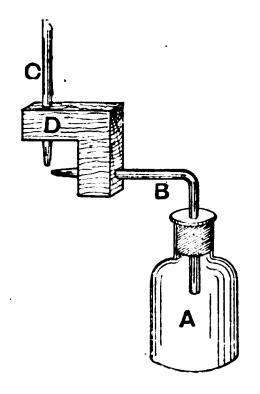
\includegraphics[width=0.4\textwidth]{Figures/_048.png}
		\caption*{Fig. 48.--Sprayer for Colouring Book Edges.}
	\end{figure}
two pieces of glass tube about 1/8-in. bore, and
D is a small piece of wood or metal. When A is
filled with ink or dye, upon blowing down C a fine
shower of spray is directed downwards. A far
neater arrangement made wholly of metal can
be bought very cheaply. Having obtained a
suitable sprayer, cover the book to be coloured
with paper, leaving only the edges bare;
take the spray producer, hold it over the book,
blow down C, Fig. 48, and the book will soon be
coloured with an even coat. If this is done for a
short time only it will give a speckled appearance.
\pagebreak
If a few grains of rice or such-like be spread along
the edges before the colour is applied, the effect
will be similar to marbling; and if it is done first
with one colour--say red--the grains of rice shaken
off, some more dropped on, and then done with
some other colour--say blue--the result will be very
pleasing indeed. Another method is to dip a
toothbrush in dye, hold it over the edges of the book,
and then draw a knitting-needle from one end of
the bristles to the other.

Sprinkled edges usually are adopted for half-calf
and cloth work. Ordinary red sprinkle may be
made of any cheap dark red pigment carefully
ground. Armenian bole (a red earth brought from
the East) is usually employed, but red ochre or
Indian red will do. The Armenian bole is poured
in a small heap on the centre of the grinding slab,
a depression is made in the centre of the heap,
and a lump of thin paste and a few drops of sweet
oil are placed therein. The whole is then mixed
well together with a palette knife into a rather
moist, red paste. The bulk of the mixture is then
pushed on one side, a lump about the size of a
walnut being placed in the centre of the slab and
ground with the muller, working with a circular
motion, until all grittiness has vanished and the
paste is quite impalpable. When sufficient of the
paste has been ground, it is placed in the sprinkle
pot, which is a red earthenware jar large enough
to contain as much sprinkle as is likely to be
needed. Water is then added, and the sprinkle
well stirred until the paste is all dissolved. The
books to be sprinkled are ranged side by side on a
bench and a cord put round them, or, better, they
are screwed up in the lying press. The operator
then takes up a brushful of sprinkle, squeezes out
the surplus on the edge of the pot, and strikes the
brush (keeping it over the pot) across a short thick
stick, held in the left hand, until the brush is only
\pagebreak
slightly charged and the spots or drops thrown off
are very small and fine. He then in the same way,
keeping his hands tolerably high, strikes the brush
forcibly against the stick, so as to send down a
shower of very small red spots upon the edges of
the book beneath. Considerable practice is required
for the proper performance of apparently so simple
an operation as sprinkling.

Although the method of preparing red sprinkle
has been described at length, the amateur will find
that almost any dye or stain (such as Judson's dyes),
diluted if necessary, can be used. Some binders
use ordinary writing ink even. A method of ornamenting
book edges that permits of a great variety
of treatment is to scatter over the edges, before
	\begin{figure}[h]
		\centering
		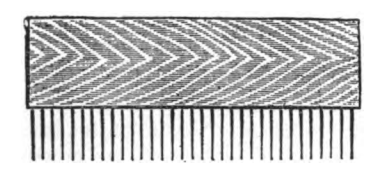
\includegraphics[width=0.6\textwidth]{Figures/_049.png}
		\caption*{Fig. 49.--Marbling Comb.}
	\end{figure}
sprinkling, rice grains and small seeds, or small
paper patterns of various shapes. By altering the
arrangement of the seeds or patterns and sprinkling
with a different colour a variety of effects can be
produced. This method is noted on p. 81. The
edges of a book should be burnished after sprinkling,
colouring, or marbling.

Another method of sprinkling, but one that is not
recommended, is this: A small brush like a sixpenny
gum brush, dipped in colour, is held tightly between
the finger and thumb of the left hand near to the
end of the hair. The forefinger of the right hand
strikes the projecting hair with a movement similar
to that employed when playing a Jew's harp. The
brush does not hold much colour owing to the
\pagebreak
manner in which it is held in the fingers, and the
workman in consequence loses time.

One, two, three, or any number of colours may
be used to the same edge, and many combinations
have a pleasing effect. A great deal depends upon.
the taste of the workman.

A good substitute for marbling, and one which
looks much better than sprinkling, is mottling. This
is done with an open-holed sponge filled with colour
and daubed lightly over the edge, leaving the
natural marks of the sponge. The edge may be
coloured all over first, or it may be mottled on the
white edge alone. Red and black makes a good
combination. This style of edge is not very suitable
	\begin{figure}[h]
		\centering
		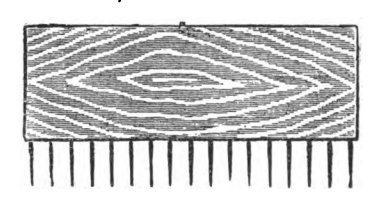
\includegraphics[width=0.6\textwidth]{Figures/_050.png}
		\caption*{Fig. 50.--Marbling Comb.}
	\end{figure}
for letterpress work, but it looks its best on heavy
account books. It is certainly much more beautiful
than some of the Dutch marble patterns seen upon
this class of work.

The marbling of book edges and the making of
marbled papers is, as may be judged from the
finished results, a difficult art. Some bookbinders
are able to do their own marbling, but, as a rule,
except, perhaps, in country places, marbling is
generally entrusted to professional marblers, who
do the work very cheaply and expeditiously.
Amateurs will do well if they also employ the
professional marbler, for though the work is not
beyond the capacity of a painstaking and artistic
amateur, it will for the majority be found tedious,
\pagebreak
messy, and probably unsatisfactory. But though
marbling requires some skill, yet it is at the same
time a simple process, and the apparatus and
	\begin{figure}[h]
		\centering
		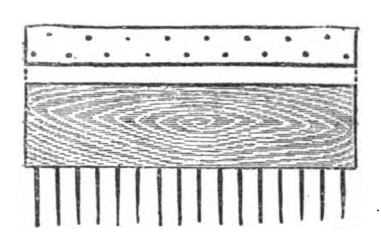
\includegraphics[width=0.4\textwidth]{Figures/_051.png}
		\caption*{Fig. 51.--Marbling Comb.}
	\end{figure}
materials may be described in a few words, all that
is necessary being a shallow wooden water-tight
trough, a flat piece of wood, equal in length to the
breadth of the trough and about 3 in. broad, a
number of combs (Figs. 49 to 51) the teeth of which
are of different widths, wooden rakes, cups, jugs,
bottles, brushes for the colours, a large earthenware
	\begin{figure}[h]
		\centering
		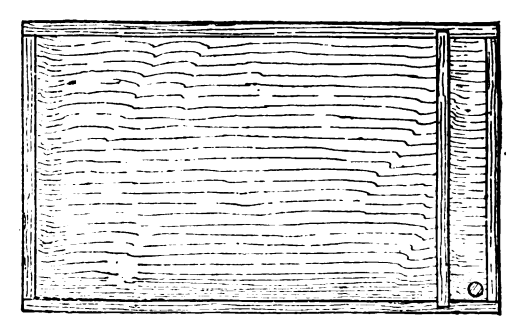
\includegraphics[width=0.6\textwidth]{Figures/_052.png}
		\caption*{Fig. 52.--Marbling Trough.}
	\end{figure}
bucket or pan, a bunch of birch rods, and a marble
slab and muller for grinding the colours. Thus it
is quite an easy matter for the marbler to construct
his own apparatus. The trough is generally of well-
\pagebreak
seasoned oak; the size is immaterial, but must be
larger than the work to be done. Useful dimensions
are about 30 in. by 18 in. or 20 in. by 2-1/2 in. It
should be made of stuff sufficiently thick to prevent
warping, and about 3 in. of its length should be
cut off by a sloping partition, which should be about
1/8 in. below the sides. In the right-hand corner of
this part a waste hole should be bored and stopped
by a cork (see Fig. 52). The joints must be well
made and stopped with marine glue or other water-
	\begin{figure}[h]
		\centering
		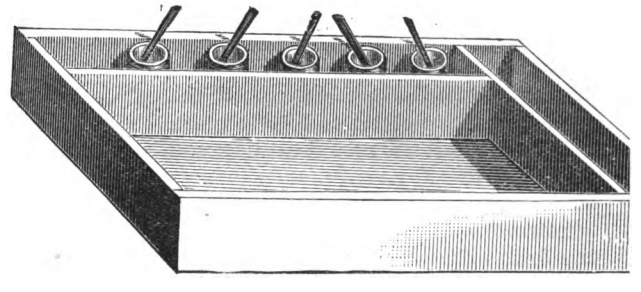
\includegraphics[width=\textwidth]{Figures/_053.png}
		\caption*{Fig. 53.--Marbling Trough and Colour Pots.}
	\end{figure}
proof material. Fig. 53 shows a marbling trough
partitioned off to hold colour bottles.

Gum-tragacanth or gum-dragon is the binding
gum used, and it should be large, white, and flaky;
dark brown lumps must be rejected. To prepare
the gum, in a large earthen pan, glazed inside, and
capable of containing, say, 12 gal. of water, put 1 lb.
of gum-dragon, and on this pour 2 gal. of soft water
(rain water if possible). Stir it every few hours
with a clean birch broom (bunch of birch rods) kept
for this purpose, breaking the lumps and adding
water as the gum thickens. The gum requires from
two to four days to dissolve properly, and must
then be strained through a fine hair sieve before
use. Other materials from which marbling size
may be made are linseed, flea-seed, and carrageen,
\pagebreak
or Irish moss, but gum-dragon cannot be excelled
for everyday work.

Generally, the marbling colours are the same as
those used for painting, both in oil and distemper.
They should be procured in the dry state and
ground by the marbler himself, although colours
are to be had ground and ready for use and put up
in air-tight jars. Following is a list of colours:
Reds--drop lake, peach-wood lake, vermilion, rose
pink, and burnt Oxford ochre. Yellows--lemon
chrome, Dutch pink, and raw Oxford ochre. Brown--
Turkey (burnt) umber. Blues-indigo, Chinese
blue, ultramarine, and Prussian blue. Blacks--
vegetable lampblack and drop ivory black. Orange--
orange lead and orange chrome. White--China clay,
pipe-clay, flake white, and Paris white.

Drop lake is the most beautiful and expensive of
the reds, the different shades being scarlet,
crimson, and purple. The scarlet possesses a brilliancy
greater than that of any other colour, and is sold in
the form of small cones or drops. To select a good
quality, break one of the little drops and try the
broken part on the tongue. If it takes up the moisture
from the tongue without any inclination to
adhere, it may be purchased. Vermilion is very
heavy, and is seldom used except in combination
with some other colour. Rose pink, a very useful
colour, is chalk or whiting coloured with Brazil
wood; it is a fugitive colour, quickly fading on
exposure to heat or even to the atmosphere, but
with Chinese blue or indigo it makes a good purple.
Burnt ochre is extensively used either by itself or
in combination with other colours; mixed with
black it makes a good brown, and with blues various
shades of olive can be obtained. Wood lake is a
damp colour, and can be used without grinding,
being made almost exclusively for marbling. It is
the best red for general purposes, and has an
appearance almost equal to drop lake. The most
\pagebreak
useful blue is indigo. It is not by any means a
bright colour, but if of the best quality it is one of
the most durable. It is invaluable for producing
greens and purples. Chinese blue is a necessary
colour, but it is not very durable. It must be well
ground, and with the addition of varying proportions
of white nearly every shade of blue can be
produced. Vegetable black will not produce a
black for marbling except in combination with
double its weight of indigo; it is much used. Orange
lead, a very heavy colour, is but little used except
for the edges of account books. White is not much
required, as with gall and water white spots can
easily be produced; however, China clay and pipeclay
are used where necessary.

For grinding colours in the dry state a marble
slab and muller must be procured. Large quantities
are treated in a colour mill, which is simply a pair
of porphyry rollers rotating in opposite directions
close together. The colour has to be passed
through several times before the proper degree of
fineness is reached. After being ground, the
colours are mixed in a cup with water. Besides the
gum or size and colours, ox-gall, ammonia, spirits
of wine, and oil will be required. Get a gall-bag
from the butcher and cut a hole in the bottom to
allow the gall to run into a bottle. Gall when new
is often thick, but it will thin and improve with
age. For the bottle get a well-fitting cork, and cut
two pieces out of the sides opposite each other;
then put the cork tightly in the bottle, and, without
removing the cork, when the bottle is turned up a
drop at a time will come out. The ammonia and
spirits of wine must be kept tight with ground glass
stoppers. Some of the colours require a little
beeswax to prevent them rubbing off and to aid in the
burnishing afterwards. It must be added while
grinding. To prepare it, chop a small piece of
beeswax fine, and place it in a small tinned iron
\pagebreak
or enamelled vessel on a stove until it is melted.
Then pour gradually into it some spirits of turpentine,
stirring all the time until it acquires the
consistency of honey. Allow it to cool, when it
can be added to any colour and ground with it when
necessary.

The operation of marbling may now be described.
With the size a little thicker than good milk, fill
the trough to within 1/2 in. of the top, pouring it
through the sieve. Take the skimmer (the flat
piece of wood already mentioned) and draw it over
the surface of the size; if considerable resistance is
felt, the size is too thick. Throw on a few spots of
colour; if these lose their shape and appear to be
attracted to the sides of the trough, the size may be
considered too thin. Again, if the colours crack
and are a long time spreading, the size is too thick.
Put into each cup or pot of colour a few drops of
gall and stir it well with a small brush, which should
be provided for each cup. There must also be a
cup of gall and water only, with a brush.

It will be impossible here to set out in detail the
manipulation of the colours to produce all the
numerous patterns of marbling, but one or two of the
commonest or best known designs will be described.
Brown shell is a simple pattern, being a brown
marble with red, yellow, and black veins. As the
brown is required to spread on the size more than
the other colours, it must be thicker, and it must
have more gall mixed with it and a few drops of
olive oil to cause the shell to be formed. Test each
colour separately on the trough, skim the surface,
and allow the waste to go over into the receptacle
at the end of the trough. Then with the red brush
sprinkle the entire surface until it is well covered;
follow with the yellow and the black, and finish
with the brown, which will spread in shell-like spots
lighter in the centre than at the edges, driving the
other colours into veins. The shell effect will vary
\pagebreak
with the amount of gall in the brown, and the larger
the shell the finer the veins. As to the quantity
of oil, if there is too little the colour will part
and produce holes here and there.

Next the book can be dipped, as in Fig. 54.
Resting the arms on the trough, dip the book from
the back to the fore-edge, making a half-circle
movement with the two hands. If the book is
dipped too much an unsightly mark will be left on
the fore-edge. After dipping, turn the book sharply
towards the body and blow strongly over the edge
to get rid of the surplus size. Sometimes it may
	\begin{figure}[h]
		\centering
		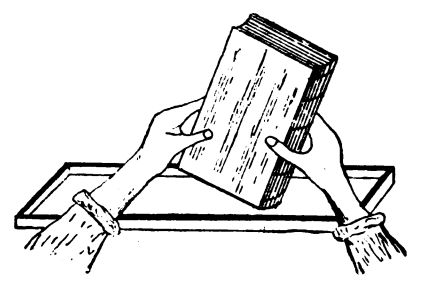
\includegraphics[width=0.7\textwidth]{Figures/_054.png}
		\caption*{Fig. 54.--Marbling Book Edges.}
	\end{figure}
be necessary to wash the size off. To do this, fill
the mouth with clean water and squirt it over the
edge, or pour the water from a cup. All these
operations must be performed quickly; a slow marbler
will never be successful. If the trough is big
enough, the three edges may be dipped one after
the other; if not, the design must be thrown on
three times, the size being skimmed after each. The
pattern can be varied indefinitely by changing, first
the vein colours and then the body colour, making
green shell, red shell, etc.

The Spanish pattern is very common, and is
known by a peculiar light and shade effect of the
body or top colour. To produce brown Spanish
\pagebreak
with red, yellow, blue, and black veins, the colours
are prepared as already described; but it may be
necessary to add more gall to some, the general rule
being to have each colour richer in gall than that
preceding it. The brown, of course, must be thickest,
and should have more gall than the others.
First throw on the red, then the yellow, and follow
with the blue and the black; sprinkle all freely, and
distribute them evenly over the entire surface. Now
with a brush well filled with brown start throwing
on the colour at the left-hand corner, working to
and from the body, and taking care not to go over
the same place twice. Finish throwing on at the
right corner farthest away. Dip the edge, but in
doing so give it a wave-like motion--that is, dip
about 1 in. of surface and draw backwards slightly
towards the right; then dip another portion and
draw back; repeat until the entire edge has been
dipped.

For nonpareil pattern a peg-rake and comb are
necessary. The peg-rake is simply a piece of wood
with pegs stuck into it. To make it, on a strip of
wood longer than the trough mark the length of
the trough, leaving equal distances at each end.
Divide the marked length equally, make a number
of holes about 1-1/2 in. apart, and in these insert
taper wooden pegs about 3 in. long. Leave one
peg out at the end, so that the rake can be moved
lengthwise the width of a peg space. The pegs
must reach to the bottom of the trough. The comb
is made in much the same way, but is only a little
longer than the breadth of the trough. The teeth
are of pin-wire, and may run from four to twelve
pins to the inch (see Fig. 49, p. 82). They should
just reach to the top of the colour when the wooden
part of the comb touches the upper edges of the
trough. All the colours for this pattern should have
about the same amount of gall and should be as
nearly as possible of the same thickness, as all are
\pagebreak
intended to spread equally. First sprinkle or throw
on the red so as to cover the entire surface; then
throw on the black, then the yellow, then the blue,
and lastly the top colour of whatever shade may be
desired. Next put the rake into the solution at the
far side of the trough and draw it carefully to the
near side, and, without lifting it out, shift its
position the width of a peg and push it back again
and lift it out. Rest the wooden part of the comb
on the edges of the trough at the left- hand side, and
draw it carefully along until the comb reaches the
right-hand side, allowing the pins just to touch the
colour; the pattern is then complete, and the book
may be dipped with a steady hand as before described.

\pagebreak

\fancyhead[CO]{\textit{MARBLING BOOK PAPERS.}}

\thispagestyle{empty}

\vspace*{\fill}

\begin{center}

\begin{large}CHAPTER X.\end{large}

\begin{small}MARBLING BOOK PAPERS.\end{small}

\end{center}

\noindent
The following information on marbling paper is
intended to supplement that already given in the
previous chapter.

Gum-tragacanth should alone be used as a
size, for most of the troubles in marbling arise
from the use of an inferior gum or the inclusion of
some other ingredient with the size. Good bright
colours must also be used, and must be well
ground; in fact, when a colour seems intractable,
sometimes the best remedy is to put it on the slab
again and grind it.

When preparing the colours specially for marbling
paper, a little beeswax is added, about
1 oz. to the pound of the colour being sufficient.
This prevents the colour rubbing off on the hand,
and causes the paper to take a better glaze when
being milled or rolled. Some colours require more
than others, the greens and blues perhaps requiring
most wax.

The illustrations here given show well-known
patterns; but before describing them it may be
stated that if, instead of a common white paper,
one covered with a coloured enamel or gold or
silver is used some very beautiful effects can be
produced.

Fig. 55 illustrates a pattern of marble paper called
"Nonpareil." To produce this pattern, besides the
colours and a brush for each, a peg-rake and fine
comb will be required. Into each cup of colour,
carefully ground and mixed with water, put a few
drops of gall and stir well with the brush to be
\pagebreak
used. Skim the surface of the trough, and throw
or sprinkle on the colour by beating the brush
against an outstretched finger of the left hand or
against an iron pin held in the left hand. Begin
with red, and sprinkle this so as to cover the entire
surface of the size in the trough, following with
black, yellow, or orange and blue, and finish with
a top colour, which may be left to the fancy of the
operator. Rake the colour with the peg-rake; that
is, put the rake into the solution at the front of
the trough and push it back, then move it to the
right about the width of a peg and draw it to the
	\begin{figure}[h]
		\centering
		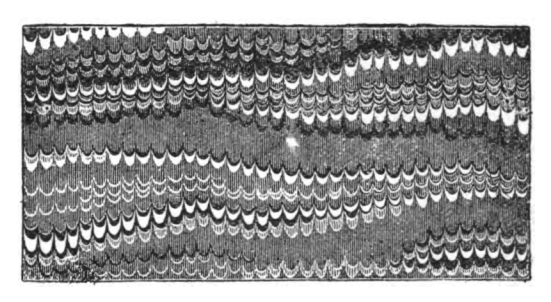
\includegraphics[width=0.9\textwidth]{Figures/_055.png}
		\caption*{Fig. 55.--Nonpareil Marble.}
	\end{figure}
front again, and lift it out. The colour will now
lie in regular streaks across the breadth of the
trough. The pegs must reach to the bottom of the
trough. Now draw the fine comb (Fig. 49, p. 82)
carefully through the colour from left to right, and
the pattern then is ready to be taken up on the
paper.

To place a sheet of paper on the marbling
colour, as the latter lies in the trough, and lift it
again after it has taken up the colour requires
some skill. By two opposite corners take up
a flat sheet of paper, hold it over the trough
until confident that the hands are in proper control,
lower the right hand until it rests on the side
\pagebreak
of the trough, and allow merely the corner of the
paper to come in contact with the solution, at the
same time lowering the left hand slowly until the
entire sheet is on the surface, and the left hand
resting against some portion of the trough. Then
raise the right hand until the sheet has been lifted
off. If the paper is too large to manage in this
way, allow it to lie on the solution, and place
across the trough from front to back a light rod
such as a lath, taking hold of the sheet by the
two right-hand corners and placing it over the rod;
then by gently raising the rod, lift the paper off
	\begin{figure}[h]
		\centering
		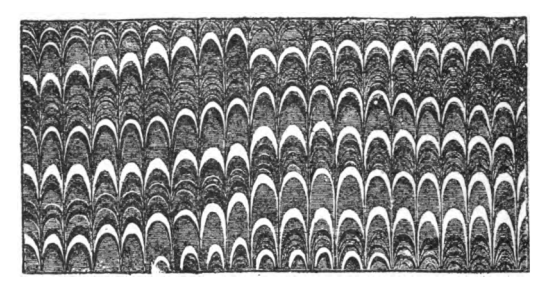
\includegraphics[width=0.9\textwidth]{Figures/_056.png}
		\caption*{Fig. 56: Reversed Nonpareil Marble.}
	\end{figure}
the trough and spread it out flat or hang it up to
dry. If the paper is lowered too quickly, the air
will get under it and produce white spots; and if,
when the paper lies on the trough, attempt is made
to get the air out, unsightly marks will be formed.
The varieties of this pattern are infinite; for
instance, any number of colours may be used, or only
one colour, hence there is blue nonpareil, black
nonpareil, etc.

Reversed nonpareil is illustrated by Fig. 56,
and for this it is usual, although not necessary, to use
a wider comb (shown by Fig. 50, p. 83), which in
this instance will be drawn through the colour from
right to left.

\pagebreak

Fig. 57 is a variety called "Wave Nonpareil."
For this, after the pattern has been produced as
already described, another comb is drawn though the
colour from right to left with a definite zigzag
movement, so as to produce even rows, which when
viewed diagonally will appear as squares. The
comb for this pattern is shown at Fig. 51, p. 84.
It may be described as a double comb, as will be
seen from the plan, the teeth of the second row
being set to come exactly in the centre of the
spaces in the first row. The teeth should not be
	\begin{figure}[h]
		\centering
		\includegraphics[width=0.9\textwidth]{Figures/_057.png}
		\caption*{Fig. 57.--Wave Nonpareil Marble.}
	\end{figure}
less than 1 in. apart, and the second row should
be at the same distance behind the first.

A very striking modification of this pattern is
called "Fancy Dutch" (Fig. 58). It may be produced
with three colours only and gall and water,
the colours being red, black, and a fancy blue (say
turquoise blue). Throw on a little of the red first,
and follow with black in about the same proportion,
but somewhat thicker, and with more gall,
so that it may spread and produce larger spots.
The blue must be still thicker than the black, as
it is required to spread still more. Finish with a
fairly liberal supply of gall and water, which must
spread more than any of the colours. This done,
\pagebreak
rake as for nonpareil, and with the double comb
finish the design.

If, instead of a white paper, a gold surface paper
is used, the effect is really beautiful, as so much
	\begin{figure}[h]
		\centering
		\includegraphics[width=0.7\textwidth]{Figures/_058.png}
		\caption*{Fig. 58.--Fancy Dutch Marble.}
	\end{figure}
of the gold surface is seen, owing, of course, to the
gall and water having been used. It need not be
stated that the size should be clean, otherwise
much of the brilliancy will be lost.

	\begin{figure}[h]
		\centering
		\includegraphics[width=0.7\textwidth]{Figures/_059.png}
		\caption*{Fig. 59.--Italian Marble.}
	\end{figure}

A very simple pattern, called "Italian" (Fig 59),
may, if desired, be produced with one colour and
gall and water. Take red, for instance, and with
this cover the entire surface of the trough; now
\pagebreak
with a large brush filled with gall and water
sprinkle carefully so as to produce very fine white
spots.

The brush used for this is an ordinary glue or
	\begin{figure}[h]
		\centering
		\includegraphics[width=0.7\textwidth]{Figures/_060.png}
		\caption*{Fig. 60.--Dutch Antique Marble.}
	\end{figure}
paste brush with an iron ring, and it should be
beaten against an iron pin as usual. The spots may
be made of irregular sizes by first having the brush
fairly wet with the gall and water, and afterwards
	\begin{figure}[h]
		\centering
		\includegraphics[width=0.7\textwidth]{Figures/_061.png}
		\caption*{Fig. 61.--Antique Spot Marble.}
	\end{figure}
almost dry, in both cases going over the whole
trough while sprinkling.

Dutch antique pattern shown by Fig. 60 is another
modification of the nonpareil series, and
the colours should be of the best, so that they
\pagebreak
may be as bright as possible. They should be of
about the thickness of cream, and are put on the
trough with little sticks or quills in sloping streaks.
For instance, put on pairs of strokes over the whole
trough, and between these double strokes put a
stroke of say orange or yellow; then fill the wider
spaces with green, blue, or black as desired, and
draw a wide comb through to complete the pattern.
If a sprinkle of gall and water is given before
drawing through the comb, and a gold or silver
	\begin{figure}[h]
		\centering
		\includegraphics[width=0.9\textwidth]{Figures/_062.png}
		\caption*{Fig. 62.--West End Marble.}
	\end{figure}
paper is used, the effect will be found to be much
enhanced.

Antique spot pattern (Fig. 61) is capable of much
variation; the spot, for instance, may be white,
pink, green, or gold. To produce it, the colours
red, black, and yellow may be thrown on in the
same or varying quantities and raked once up and
down; afterwards another colour, blue or green,
may be thrown on; then the pink for the spot, or
gall and water, which will produce white if white
paper is used, or gold if a gold surface paper is
preferred.

West End pattern, shown by Fig. 62, is also
capable of much variation, but commonly consists
of two prominent colours besides the veins, one of
the colours, generally the darker, being spotted
\pagebreak
finely with white. To produce this pattern, mix
the colours red, black, and yellow, or as desired,
for veins, and throw them on the trough, red first.
Then mix, say brown, with a larger proportion of
gall and sprinkle it on in large, full spots, so as
to drive the other colours into veins. Now with
a large brush, well filled, sprinkle gall and water
over the entire surface. When well beaten out
against the iron pin, the brush will produce very
fine spots. Then take some white and mix it with
	\begin{figure}[h]
		\centering
		\includegraphics[width=0.9\textwidth]{Figures/_063.png}
		\caption*{Fig. 63.--Machine-pattern Marble.}
	\end{figure}
the brown so as to make it lighter, adding also a
drop or two of gall; sprinkle this on full so as to
produce large light spots, which complete the pattern.
Some of the newer patterns of marble papers
are produced by mechanical means. One machine
works somewhat like the air-brush, the colour being
blown on to the paper and making a pattern like
Fig. 63.

It is often necessary to size the paper after
marbling, and before milling or glazing, and the
best way to do this is to fill the trough with size
and place the paper on it as for marbling. Of the
many sizes, glue is always the basis. An old-fashioned
\pagebreak
recipe may be quoted: "Take of the best
white soap 2 lb., put it into a large copper with
about 20 gals. of water, and when it is quite
dissolved add thereto about 4 lb. of best glue,
keeping the whole constantly stirred to prevent burning.
When both are quite dissolved strain into a tub,
and when cool the mixture is ready for use." After
sizing, the paper is passed through a calendar, that
is a machine with polished steel rollers and with
appliances for heating, so as to give a good gloss
to the paper.

\pagebreak

\fancyhead[CO]{\textit{GILDING BOOK EDGES.}}

\thispagestyle{empty}

\vspace*{\fill}

\begin{center}

\begin{large}CHAPTER XI.\end{large}

\begin{small}GILDING BOOK EDGES.\end{small}

\end{center}

\noindent
Gilding is the most beautiful method of ornamenting
the edges of books; it suits almost any colour
and any binding, and may be carried out in a
variety of ways so as to produce many beautiful
effects. Gilding is not mere ornamentation; it is
also the best preservative that can be applied to
book edges. Dust cannot penetrate between the
leaves of gilt- edged books, decay is retarded if not
altogether prevented, and the action of fire is
resisted to a remarkable extent; it is for this last
reason that the edges of ledgers are sometimes very
thickly gilt. Among the many varieties of gilding
may be mentioned gilt on colour, in which the edges
are fanned out and coloured, and then gilt. Red is
the colour most generally preferred, hence the
common expression "gilt on red," or "red under gold";
but other colours are used. Gilding is also done
on marble; it is called marbling under gilt, and as
may be imagined, when well done is very beautiful.
Book edges are also gilt and tooled, tools of a fine
pattern being chosen and used warm.

The tools used by the edge gilder for ordinary
plain gilding are the gilding press, which has long
screws, a steel scraper, a gold cushion, gold knife,
tip, burnisher, and a flat brush. The materials
required are gum, Armenian bole, diluted glaire, and
gold leaf.

In shops where gilding is done only occasionally,
the ordinary lying press may be used in place of
the gilding press. But where large quantities of
work are executed it is usual to have a special
press of the kind shown by Fig. 64.

\pagebreak

The ordinary steel scraper is shown by Fig. 65,
and is simply a flat piece of steel about 1/32 in.
thick. The scraper can easily be made from a broken
knife, which should be ground up in the same way
	\begin{figure}[h]
		\centering
		\includegraphics[width=0.6\textwidth]{Figures/_064.png}
		\caption*{Fig. 64.--Gilder's Press.}
	\end{figure}
as a carpenter's chisel, except that the corners
should be rounded a little. Many workers prefer
it ground up while soft, so as to cast a "burr" upon
the edge, and then hardened; the burr thus produced
is used to scrape with, and a scraper thus made
will be found to cut very quickly.

	\begin{figure}[h]
		\centering
		\includegraphics[width=0.3\textwidth]{Figures/_065.png}
		\caption*{Fig. 65.--Steel Scraper for Book Edges.}
	\end{figure}

The book edge gilder's gold cushion, illustrated
by Fig. 66, resembles that used by the painter and
decorator, and consists of a flat board measuring
about 1 ft. by 9 in. or so, with two or three thicknesses
of flannel or printers' press-blanket laid flat
upon it, and then covered with a piece of calf-skin,
\pagebreak
flesh or rough side upwards, nailed down to the
edges of the board.

To make a gold cushion, take a piece of wood,
size immaterial--12 in. by 6 in. by 1 in. does very
well--and lay upon it several sheets of blotting-
paper, the bottom one the same size as the wood,
the next a shade smaller, the next smaller still, and
so on until enough is laid on, and then cover with
a piece of calf, the rough side up, and fasten it on
by nailing it all round the edge. A slip of stout
	\begin{figure}[h]
		\centering
		\includegraphics[width=0.7\textwidth]{Figures/_066.png}
		\caption*{Fig. 66.--Gilder's Cushion.}
	\end{figure}
vellum is generally placed along the edge outside
the leather, and nailed through with brass nails
with big convex heads, such as upholsterers use for
brass-nailing chairs. Decorators and gilders generally
protect the cushion with a screen of stout
vellum a few inches high, but as the finisher does
his work indoors a screen is hardly necessary; it
is, however, shown in the illustration (Fig. 66).
Gold cushions can be purchased of any artists'
colourman, and of many oilmen. The knife is about
\pagebreak
the shape of a palette knife (see Figs. 67 and 68),
with a somewhat rough (but not too rough) cutting edge.
The tip (Fig. 69) is similar to that used by the
decorator and gilder, and consists of a few hairs
of sable secured in a cardboard handle. It is
used for lifting the gold leaf, but many finishers
prefer a bit of cotton-wool or wadding, rendered
slightly greasy by being passed across the forehead.

	\begin{figure}[h]
		\centering
		\includegraphics[width=0.6\textwidth]{Figures/_067.png}
		\caption*{Fig. 67.--Gilder's Knife.}
	\end{figure}

The steel burnisher used is illustrated by Fig.
70; it has a wooden handle.

All the gilding done in the finishing of books is
executed with gold leaf. The gold leaf is put up
into small paper books, each containing twenty- five
leaves of gold, and is sold by the hundred leaves
(four books). Gold leaf varies in colour according
to the manner in which the metal is alloyed before
being beaten out. The different tints are deep
gold, ruddy orange, medium gold, pale gold, and
pale lemon. Generally deep gold is preferred by London binders.
	\begin{figure}[h]
		\centering
		\includegraphics[width=0.6\textwidth]{Figures/_068.png}
		\caption*{Fig. 68.--Gilder's Knife.}
	\end{figure}
With regard to preparing the edges to receive
the gold, screw the book into the press, with the
edge to be gilt level with the top of the press,
carefully ascertaining that the leaves are quite
level with each other, and then give it a coat of
size. The fore-edges are first dealt with. When
the size is dry, scrape the edge until all irregularities
of the leaves disappear. The scraper, which
\pagebreak
should not have a very sharp edge, is held between
the thumbs and fingers of both hands in an
inclined position, and is worked, with some amount
of pressure, along the edges of the book in a
direction away from the operator. The scraping is
continued until the edges are perfectly level and
smooth. To gild edges that have not been properly
treated at this stage will simply be a waste of
gold.

A little Armenian bole or red ochre, mixed with
a little thin glaire, is smeared over the edges with
\begin{figure}[h]
	\centering
	\includegraphics[width=0.55\textwidth]{Figures/_069.png}
	\includegraphics[width=0.17\textwidth]{Figures/_070.png}
	\caption*{
		Fig. 69.--Gilder's Tip.
		Fig. 70.--Gilder's Burnisher.
     }
\end{figure}
a bit of sponge, and then wiped off as clean as
possible with a bunch of clean shavings. When
dry the edges are burnished. This red ground
forms a good foundation for the gilding. The
edges are then glaired, and the gold leaf is applied.

An alternative method of treating the edges after
scraping is to mix a small portion of size with a
little blacklead until they form a paste; brush some
of this on the edge quite evenly, and then brush
briskly with a hard brush until dry. If the edges
now present an even appearance--no parts being
\pagebreak
left unblackleaded--apply first a coat of glaire and
then the gold-leaf.

Before using the gold cushion its surface should
be rubbed over with some Armenian bole or
powdered red ochre to prevent the gold adhering
to the cushion should the latter be in any way
greasy. A leaf of gold is then placed on the
cushion and made to lie flat and smooth by blowing
gently on the centre of the leaf. The leaf is then
cut to the desired size, the edge of the knife being
sharp, but not too keen. The tip or cotton-wool is
made slightly moist or greasy by drawing it across
the forehead; this is done so that the gold-leaf may
readily adhere to the tip; or instead cut a piece
of writing-paper a little larger than the strips of
gold-leaf, and rub it on the hair to make it slightly
greasy. There is enough natural grease in the hair
of everyone for the purpose mentioned, only the
slightest possible amount being needed. The leaf
is now picked up by pressing the paper into contact
with it, and laid in its place on the book edges.

Suppose it is necessary to use three half-leaves
of gold to cover the edge. Lay out two leaves on
the cushion and cut both in half with the knife.
Supposing pieces of paper to be used, lift up a
piece of gold, which then will adhere to the paper.
Lay this down, gold upward, and lift the other two
pieces in like manner. Now well fill the size brush
(a flat camel-brush), and pass it quickly over the
edge with one sweep if possible, taking care not
to disturb the blacklead; then as quickly as
possible lift the gold now on the papers and lay
each piece upon the edge. Care must be taken to
prevent making holes in the leaf, and the various
pieces must overlap but slightly. Holes that have
to be patched generally are unsightly, as also are
broad overlaps.

If time can be allowed, it is best to protect the
\pagebreak
edge from dust and to allow the gold to dry
naturally. This may take from three to six hours,
according to the atmosphere of the room in which
the operation is carried on. When dry the gold
must be burnished. The burnisher should be used
in somewhat the same manner as a cobbler burnishes
the edges of a boot sole; the main thing is
a fair amount of pressure applied evenly. If the
gold is to be bright, the edges must be rubbed over
with a waxed cloth before burnishing; dull gilt is
produced by keeping a piece of paper between
the gold and the burnisher. The edges are then
papered up until the binding of the book is completed.
The method of burnishing adopted by some
bookbinders is as follows. Before burnishing the
gold is rubbed down with a piece of paper held in
the left hand; then place the paper upon the edge
and rub the burnisher over it. The edge must be
rubbed over with something to prevent the burnisher
sticking, beeswax being generally used. A
little is rubbed on the cheek of the press in a
convenient position for the right hand, and a piece of
leather or the fleshy part of the hand is rubbed
over the wax, and the edge is rubbed with this.
The burnisher is grasped in the closed hand and
held by the thumb and forefinger; it comes out
between the first and second fingers. The handle
is placed against the shoulder, and this indicates
that considerable pressure is to be used in this
operation. The burnisher is passed forwards and
backwards across the edge. This motion is kept
up until a high degree of polish is obtained,
rubbing being done now and again with the wax if
required.

Sometimes, especially in devotional books, emblems
and devices are painted in water-colours on the
gilt fore-edges. Another plan, effective but
expensive, and therefore seldom resorted to, is to
\pagebreak
fan out the edges, and paint on them in watercolours
a landscape, figures, or appropriate floral or
other patterns and devices. The book is then
gilded on the edges in the usual manner. A specimen
can be seen in the Guildhall Library, London,
E.C.

The "red under gold" effect is produced by
reddening the edges first. Other colours are often
used, such as "green under gold," etc., but the
method is the same in all cases. For red, get a
sufficient quantity of vermilion (a dry colour in
powder), place it on a stone slab, mix it into a
paste with water, and with a stone muller grind
it until it is very fine and smooth. Then mix it in
a cup with glaire thin enough to be applied with a
sponge. This done, take the book (which must be
cut on all edges) and place it on the bench,
opening it from about the middle so that the same
number of leaves may lie to right and left. Put a
backing board on the right-hand side of the open
leaves flush with the edge, press it down tightly
with the left hand, and with a sponge dipped in
the colour put an even coating over this part of
the book edge. By this method the sides of the
edges of the book are coloured and will always
show when the book is open, which is the effect
desired. Then turn the book round and treat the
left-hand side in the same manner, and when dry
close the book, turn it round, open again, and
colour the other side of the edges. This completes
the fore-edge of the book. The ends will be more
difficult to manipulate. With the book flat on the
bench and with the fore- edge towards the operator,
take the right- hand corner of the book between the
thumb and finger of the right hand and move it
towards the left, pushing the top part of the book
backwards, and when in this position hold it so
with the left hand. Then put the backing board
on as before and colour this edge. Turn the book
\pagebreak
over and repeat the moving process in the opposite
direction and again apply the colour. The
other end is treated in the same way. When
the edges are dry, the book is put into the press
and the ordinary gilding operations are proceeded
with.

\pagebreak

\fancyhead[CO]{\textit{MARBLING BOOK COVERS.}}

\thispagestyle{empty}

\vspace*{\fill}

\begin{center}

\begin{large}CHAPTER XII.\end{large}

\begin{small}SPRINKLING AND TREE MARBLING BOOK COVERS.\end{small}

\end{center}

\noindent
The Covers of books bound in plain uncoloured calf
or sheepskin are sometimes sprinkled in order to
relieve the monotony of a plain unornamented surface.
But the custom is not so common now as it
was fifty or more years ago. Very pretty effects
can, however, be produced in this way. The
materials and the methods employed are the same
as adopted for sprinkling book edges.

Sprinkling on panels, as illustrated by Fig. 71
(see opposite page), is a style of ornamentation that
may be made very effective. By calling the work
a kind of stencilling, the manner of doing it is
explained. Such panels, borders, or other patterns
are afterwards blind-tooled by the finisher.

The marbling of the covers of leather-bound
books is produced by the application of solutions
of pearlash and green copperas. The book is
supported open as for sprinkling. The operator dips
into clean water a coarse brush or a bundle of
feathers tied together, and throws some large drops
of water on the book. As the covers are extended
in a slanting position, these drops of water run
down and form irregular rivulets. A smaller brush
is then dipped into a strong solution of pearlash
(potash), with which the cover of the book is lightly
sprinkled, and lastly a solution of green copperas
is added with a still smaller brush. All this is
done so quickly that the drops of water trickling
down carry with them some of each of these solutions
and stain the leather a rich brown (pearlash)
and black (copperas). The cover is then well
sponged with clean water.

\pagebreak

Tree marbling is formed on calf-bound books in
much the same manner as ordinary sprinkling,
except that the boards are bent outwards to allow
the water and colours to run to the centre and
produce what seem to be the branches of trees.
The name is also given to such processes as
endeavour to imitate the grain of wood. As the success
of the processes often depends on the quickness
with which they are executed, it is important that
	\begin{figure}[h]
		\centering
		\includegraphics[width=0.3\textwidth]{Figures/_071.png}
		\caption*{Fig. 71.--Sprinkling on Panels.}
	\end{figure}
the colours, sponges, brushes, etc., are easy of
access.

For this work the books are bound with what
is termed fair calf, this being leather which has
not been dyed. First the books must be carefully
washed with paste water containing a little salts of
tartar and then left to dry. Some workers also
coat them with glaire, but this, whilst allowing the
colours to flow freely, has a tendency to prevent
them striking in where wanted. When thoroughly
dry the volume is placed between marbling rods,
the sides of the book hanging over with the leaves
between the rods as shown in Fig. 72.

The rods should slope so as to allow the water
to run gradually towards the bottom of the book,
\pagebreak
and if the back is to be left plain it must be covered
with a piece of millboard or strawboard shaped
to suit.

To avoid the scum which is caused by the beating
of the brushes over the colours, it is better to rub
the ends of the bristles on the palm of the hand,
on which a little olive oil has been spread. The
brushes should be such as are used for sprinkling
edges, and should be bound with iron rings. A
bunch of quills or birch rods will also be required
for throwing on the water.

For ordinary work, with the book on the rods,
throw on the water in large drops until these unite.
Then a number of fine streaks are produced by
throwing colour evenly over the entire cover, using
a brush charged with brown liquid and beaten on
the press-pin as when sprinkling edges. Afterwards
the black liquid must be similarly thrown over.
This must be done quickly; in fact, while the water
continues to run.

Marbling water should be soft, and should have
added to it a few drops of salts of tartar. Brown
colour is prepared by dissolving 1/2 lb. of salts of
tartar in 1 quart of water. For black colour, dissolve
1/2 lb. of green copperas in 2 quarts of water. A
good blue colour may be prepared by mixing 1 oz.
of powdered indigo with 2 oz. of oil of vitriol and
letting it stand for twenty-four hours and then
adding 12 oz. of pure water. One of the best yellow
colours is prepared from hay saffron. Put a small
quantity in a cup or similar vessel, fill up with
water, and set beside a hot stove and allow to infuse.
The quantities are immaterial, as the liquid
can be made of whatever strength desired by simply
adding water to the stock solution, which should
be kept in a bottle. For green colour, liquid blue
and yellow mixed will suit all purposes. For red
colour, boil 1/2 lb. of Brazil wood and 8 gr. of
nutgalls, both powdered, in 3 pints of water; let it boil
\pagebreak
for a considerable time until it is reduced about
one-third, and then add 1 oz. each of powdered
alum and sal-ammoniac, and when dissolved strain
through a sieve. This must always be used warm.
Orange colour is produced from red and yellow
liquid.

These colours should all be kept in well-corked
bottles and in a dark place, if possible. They can
be used full strength or diluted with water if
desired.

In addition, an acid of some kind is necessary for
the work. The safest to use is oxalic acid, of
	\begin{figure}[h]
		\centering
		\includegraphics[width=0.8\textwidth]{Figures/_072.png}
		\caption*{Fig. 72.--Book between Marbling Rods.}
	\end{figure}
which a saturated solution should be kept in use;
a few drops only should be added to the water.
The proportion should not exceed one of acid in
twenty of water, otherwise the leather may be
corroded or destroyed.

For walnut effect, throw on the water in large
spots and then quickly sprinkle with brown first,
and afterwards with black. For cedar, sprinkle
as for walnut, and, before the cover is perfectly
dry, in various places on the cover daub lightly
with an open-holed sponge dipped in orange so as
to form a cloud effect. When this is dry, apply
red as nearly as possible on the same places, and
when perfectly dry give the whole two or three
coats of yellow, taking care that each coat penetrates
\pagebreak
evenly into the leather. For mahogany, act
as for walnut, but sprinkle the black more boldly,
and, when the work is dry, give two or three coats
of red. For box, the boards must be bent in five
or six different places; then proceed as for walnut.
After the work is perfectly dry, throw water in
large drops and sprinkle small spots with weak
blue; when the work is dry, apply red with a
sponge as directed for the cedar. Finally, when
dry give two or three coats of orange.

\pagebreak

\fancyhead[CO]{\textit{FINISHING BOOK COVERS.}}

\thispagestyle{empty}

\vspace*{\fill}

\begin{center}

\begin{large}CHAPTER XIII.\end{large}

\begin{small}LETTERING, GILDING, AND FINISHING BOOK COVERS.\end{small}

\end{center}

\noindent
Finishing includes all the methods employed for
decorating the cover of a book. The most usual
form of decoration consists in impressing on the
book cover, in leaf metal (gold, silver, or other
suitable metal), various designs of an ornamental
character. A similar impressed design, with the
metal leaf omitted (called blind work), is also
employed. Book covers are also decorated with
superimposed metal ornaments, which are riveted on.
Ivory and other materials are also employed for
purposes of ornamentation; but the most usual
form of decoration is by gilding and blind work.
The finishing of leather books is imitated in cloth.
In the former, all the decoration is done by the hand
of the workman, the design being worked out or
built up bit by bit; in the latter, the ornamented
cover is produced in a mechanical manner by printing
from an engraved block. The comparing together of
two ornamented books, one cloth and one leather,
will enable even a superficial observer to see
the difference in the style of decoration, and
will give some idea, too, of the great number and
the variety ofthe tools required by the finisher. The
more necessary of these numerous tools are described below.

The finishing press is a small screw press
(Fig. 73), smaller and less powerful than the ordinary
lying-press; it stands on the bench or counter at
which the operator works.

The finishing stove is used for heating the tools,
and generally is a specially contrived gas stove.
Fig. 74 shows a small one that can be stood on the
\pagebreak
	\vspace*{\fill}
	\begin{figure}[h]
		\centering
		\includegraphics[width=0.6\textwidth]{Figures/_073.png}
		\includegraphics[width=0.6\textwidth]{Figures/_074.png}
		\caption*{
			Fig. 73.--Finisher's Press.
			Fig. 74.--Finisher's Stove.
         }
	\end{figure}
	\vspace*{\fill}
\pagebreak
work-bench or on a tall tripod. An ordinary oil
stove can, of course, be used if gas is not available.

The fillet (Fig. 75) is used for gilding plain lines
on the backs of books. The tool is simply a small,
\begin{figure}[h]
	\centering
	\includegraphics[width=0.5\textwidth]{Figures/_075.png}
	\includegraphics[width=0.5\textwidth]{Figures/_076.png}
	\caption*{
		Fig. 75: Fillet.
		Fig. 76: Lines made with Fillets.
	}
\end{figure}
freely revolving brass wheel mounted in an iron
carriage that is fixed in a strong wooden handle.
Fillets of various kinds are made; they are known
as thin, thick, extra thick, thick and thin, etc., and
\begin{figure}[h]
	\centering
	\includegraphics[width=0.5\textwidth]{Figures/_077.png}
	\caption*{
		Fig. 77. Line made with Pallet.
	}
\end{figure}
one-, two-, and three-line fillets. A few examples
of the lines (Figs. 76 and 77) produced by different
\begin{figure}[h]
	\centering
	\includegraphics[width=0.2\textwidth]{Figures/_078.png}
	\caption*{
		Fig. 78. Pallet.
	}
\end{figure}
fillets will also illustrate the manner in which the
tool is employed.

The roll is also a brass wheel, similar to a fillet,
but broader in the rim. Instead, however, of tracing
\pagebreak
lines, the roll reproduces any ornamental designs
that have been cut upon its surface by the bookbinder's
tool cutter.

The general form of pallets, which are of various
	\begin{figure}[h]
		\centering
		\includegraphics[width=0.125\textwidth]{Figures/_079.png}
		\includegraphics[width=0.1\textwidth]{Figures/_080.png}
		\includegraphics[width=0.1\textwidth]{Figures/_081.png}
		\includegraphics[width=0.1\textwidth]{Figures/_082.png}
		\includegraphics[width=0.1\textwidth]{Figures/_083.png}
		\includegraphics[width=0.1\textwidth]{Figures/_084.png}
		\caption*{Figs. 79-84.--Pallet Patterns.}
	\end{figure}
sizes, is shown by Fig. 78. The shape of the tool
suggests the manner of using it. The variety of
patterns that may be cut upon pallets is infinite, from
	\begin{figure}[h]
		\centering
		\includegraphics[width=0.4\textwidth]{Figures/_085.png}
		\caption*{Fig. 85.--Line Tools.}
	\end{figure}
the most simple zig-zag to a broad belt of flowers and
leaves. Figs. 79 to 84 show simple but useful
patterns.

Line tools are shaped something like pallets, but
\pagebreak
are made in sets of ten or a dozen tools of various
lengths. Specimens of the lines produced by them
are shown by Figs, 85 to 87.

	\begin{figure}[h]
		\centering
		\includegraphics[width=0.3\textwidth]{Figures/_086.png}
		\includegraphics[width=0.3\textwidth]{Figures/_087.png}
		\caption*{
			Figs. 86 and 87.--Line Tools.
		}
	\end{figure}
	
Gouges (Figs. 88 and 89) are curved line tools.
They are made in sets, and also in various curvatures,
from a quarter-circle to a complete circle.
	\begin{figure}[h]
		\centering
		\includegraphics[width=0.4\textwidth]{Figures/_088.png}
		\caption*{Fig. 88.--Lines made with Gouges.}
	\end{figure}
These tools are of great use in patterns made by the
combination of straight lines and curves.

	\begin{figure}[h]
		\centering
		\includegraphics[width=0.4\textwidth]{Figures/_089.png}
		\caption*{Fig. 89.--Lines made with Gouges.}
	\end{figure}

Drop tools, flowers, and other ornamental separate
tools are used in great variety. In an elaborate
\pagebreak
design, every ornament may require a separate tool,
and the binder's tool cutter is always at work.
Fig. 90 is an example of a small finishing tool.
The ends of tools for producing corners and
centres are shown in Figs. 91 to 94, and being repeat
tools, four impressions of each will produce a centre.
Other simple designs are shown by Figs. 95 to 98.
To show how the above tools are used on the
	\begin{figure}[h]
		\centering
		\includegraphics[width=0.4\textwidth]{Figures/_090.png}
		\caption*{Fig. 90.--Small Finishing Tool.}
	\end{figure}
covers of books is unnecessary, when so many examples
can be seen in the shop windows of high-class
booksellers and in bookbinders' show-cases. One
example, however, of a book back may be given
(Fig. 99), and from it will be seen how it is possible
to produce elaborate effects by combinations of
simple ornaments.

Finishing requires not only careful attention in
every detail, but a considerable amount of taste and
	\begin{figure}[h]
		\centering
		\includegraphics[width=0.25\textwidth]{Figures/_091.png}
		\includegraphics[width=0.15\textwidth]{Figures/_092.png}
		\includegraphics[width=0.15\textwidth]{Figures/_093.png}
		\includegraphics[width=0.2\textwidth]{Figures/_094.png}
		\caption*{Figs. 91 to 94.--Corner Patterns, Four of each making Centre Patterns.}
	\end{figure}
ability; taste to form a true estimate of what will
harmonise with the nature of the work and add to
the beauty of the binding, and ability to execute the
designs.

According to the custom of the shop (see p. 64),
the finisher's first business may be to examine the
book critically, and if he finds any defects in the
\pagebreak
	\vspace*{\fill}
	\begin{figure}[h]
		\centering
		\includegraphics[height=0.6\textheight]{Figures/_095-098.png}
		\includegraphics[width=0.25\textwidth]{Figures/_099.png}
		\caption*{
			Figs. 95 to 98.--Cover Ornaments.
			Fig. 99.--Finished Back of Book.
		}
	\end{figure}
	\vspace*{\fill}
\pagebreak
forwarding he should point them out. With a bandstick
(a piece of hard wood about 10 in. by 1 in. by 1/2
in. planed square) the leather is rubbed close into
the sides of the bands, providing there are bands.
If the book is bound in calf, a small piece of thin
leather of a colour harmonising with the colour of
the cover is cut out, pared neatly, and pasted on
where the title is to appear (see p. 62).

Morocco and roan binding seldom have coloured
titles, so they are not "pieced," as it is termed.
The book should next be trimmed, that is, all
inequalities left by the forwarder in the cover should
be pared evenly by the finisher. Backs, corners,
sides, and insides should be treated in this manner,
for a bad appearance is given to a finished book by
lumps of leather showing beneath the cloth or paper
of the sides or insides. The board should be
opened, one of the end papers torn out (back and
front) and laid aside for lining the boards
afterwards and the joints scraped to take away any
little pieces of paste or glue that may have lodged
there. The end paper which is to be pasted to the
board should be trimmed at the sides, so that it will
be at equal distances all round from the edge of the
board. Attention to these little matters, although
they may seem trivial, will go a long way in adding
to the beauty of the finished volume. But it may be
that all the finisher will be required to do is to
proceed at once with the finishing directly he
receives the book.

All leather-bound books are washed with pastewater,
that is, clear water with a little paste mixed in
it. This replaces, or in some cases supplements,
the vellum size used formerly.

Calf, because of its great porosity, requires to be
well rubbed with paste before washing. Paste the
back with the brush, and rub the paste well into the
leather with the folder, taking care not to rub too hard.
Sometimes a little oxalic acid is added to the
\pagebreak
paste-water, and this helps to clear the lighter
colours of leather. Discretion will have to be used
in this matter, as the acid will destroy some colours.
For lettering the backs of books, at one time each
letter of the alphabet was mounted as a separate
tool, and this plan still occasionally is met with.
	\begin{figure}[h]
		\centering
		\includegraphics[width=0.5\textwidth]{Figures/_100.png}
		\caption*{Fig. 100.--Letter Holder.}
	\end{figure}
The modern plan is to cut the letters in brass type
and use them in a typeholder. The ordinary types
employed in printing are also sometimes used.
They are arranged in a holder (Fig. 100), and may be
spaced out to fill the width of the back or put close
together, as may be found necessary.
\pagebreak
Small implements and utensils also are necessary.
An earthenware pipkin, glazed inside, is required for
boiling the size. It should be provided with a flat
tin lid. An instrument called the "devil" (Fig. 101)
is used in preparing the glaire, which can be kept
in any small earthenware vessel; the devil consists
of two pieces of quill fastened as shown to a long
stick like a penholder. It is used like an egg whisk.
Two polishers used for polishing and smoothing the
back and sides of the book after finishing are shown
in Figs. 102 and 103. Fig. 102 is the polisher generally
preferred by London binders, and is very useful
	\begin{figure}[h]
		\centering
		\includegraphics[width=0.25\textwidth]{Figures/_101.png}
		\caption*{Fig. 101.--Devil for Preparing Glaire.}
	\end{figure}
for working close to the bands, but the one shown by
Fig. 103 is very good for the sides of whole-calf
volumes. Some pieces of sponge, two or three
camel-hair pencils, a gold rag, several small pieces
of flannel, and a bit of good raw rubber are also
required. The materials used by the finisher are
few, and, with the exception of gold leaf, are of little
value.

Finishers' size is made from waste slips of vellum.
which are cut up very small, put with sufficient
water into a clean pipkin, and allowed to boil gently.
It will not keep long, and fresh size should be made
often.

\pagebreak

Glaire is made by breaking the white of a fresh
egg into a tea-cup, carefully excluding the yolk,
	\begin{figure}[h]
		\centering
		\includegraphics[width=0.25\textwidth]{Figures/_102.png}
		\includegraphics[width=0.25\textwidth]{Figures/_103.png}
		\caption*{Figs. 102 and 103.--Polishers.}
	\end{figure}
adding water until the cup is about half full, beating
well together, and adding a pinch of salt as a
preservative. This having been allowed to stand for a
\pagebreak
few hours, is carefully strained through a piece of
old linen and bottled for use. No particle of the
yolk should be mixed with the white. A usual
method of making the glaire is by rolling the devil
with a rapid motion between the palms of the hands,
the quills being in the albumen. When all the
albumen has been beaten to froth it is put aside to
settle, and the result is glaire. The original white
of eggs is ropy and gelatinous, but the frothing up
makes it as thin and fluent as water. Another
method is to place the whites of two or three eggs
in a cup, and add a small quantity of vinegar and a
pinch of salt, beating the whole well together. At
the end of a minute or two remove the froth from
the top and place the preparation in a bottle.

The glaire, when ready, is applied all over the
cover of the book with a small sponge. When the
first coat is thoroughly dry give it another.
The back or side of the book on which the gold
is to be affixed must be slightly greased after the
application of the last coat of glaire. Finishers
differ somewhat as to the material to be employed.
Olive oil is used by, perhaps, most workmen; lard,
or composite, or some kind of palm-oil candle is also
used. But the quantity required is so small that
any tolerably pure fatty or oily substance will do.

Sometimes, in order to add to the glossy appearance
of calf backs, and also in some degree to serve
as a preservative coating, some kind of fine spirit
varnish is applied to the leather. The varnish
should be of the best quality, both as regards the
spirit used as a solvent, and the copal, mastic, or
other gum dissolved in it.

Suppose, as a sufficiently typical example, that
the finisher is about to deal with a batch of from
twelve to twenty half-calf books. The first operation
is to paste-wash the leather. A small quantity
of thick paste is applied to the back of the book, and
rubbed up and down the back with a folding-stick.
\pagebreak
This forces the paste into and fills up the small
pores of the leather, and thus forms a foundation for
the succeeding operations. The paste is then
washed off the back with a sponge and clean water,
the sides of the back and the corners being also
wiped over with the pasty water in the sponge.
When dry, the leather is sponged over with warm
size, and, when the size is dry, the glaire is applied
with a bit of sponge (kept specially for that purpose),
or with a camel-hair pencil.

The best procedure for ordinary half-calf work
(or for whole calf where there is to be no finishing on
the sides) is, for the first application, to go over all
the leather with the glaire. When this coating is
dry, a second coat is applied, this time to the back
only. A third coating can be given, either to the
entire back, as in the previous application, or merely
across the lettering piece. When the backs of the
books are sufficiently dry, a piece of cotton-wool to
which the least touch of oil or lard has been applied
is passed rapidly over all the surface that is to be
gilded. The strips of leaf are lifted to the place
that is to be gilded either with the tip or with a bit
of cotton-wool, the slight oiling the cover has
received causing the leaf instantly to adhere where it
is placed.

The books are now ready for the next stage. It
should be remarked here, however, that until the
amateur has acquired some experience, he will do
well to mark lightly on the back or cover, as the case
may be, with a folder, the positions the ornaments
and lettering are to occupy. The advisability of
working from a sketch plan will also be evident.
The good appearance of even excellent ornamentation
on a book cover, as elsewhere, will be marred and
probably spoilt if the arrangement is not symmetrical.
Pressure with hot tools causes the gold leaf to
adhere to the leather, and reproduces at the same
time the pattern engraved on the tool. The heat
\pagebreak
of the tool is tested with a drop of water, which, if
the tool is hot enough, should evaporate quickly
without hissing; if the water hisses, the tool is too
hot.

Suppose a volume to be screwed up in the finishing
press (Fig. 73, p. 116), which is lying on the bench
in front of the worker, the head of the book being
towards the right hand; the heated fillet is taken
from the stove, and the edge of the fillet, which
must be perfectly clean and bright, is drawn quickly
over the palm of the left hand to aid the adhesion
of the gold. The fillet is then rolled carefully over
the slips of gold leaf, which will adhere to the fillet
	\begin{figure}[h]
		\centering
		\includegraphics[width=0.4\textwidth]{Figures/_104.png}
		\caption*{Fig. 104.--Method of Holding Lettering Tool.}
	\end{figure}
till its periphery is covered. Then turning to the
book, hold the bottom of the handle of the fillet with
the right hand, allow the upper part of the handle to
rest against the right shoulder, and roll the fillet
over the back of the book at the places marked for
the bands. Having thus filleted the back seven
times (if an octavo), the finisher shifts the press so
that the tail of the book is towards him, raises the
head of the book somewhat higher than the tail, so
that the back is rather inclined, and then proceeds
to apply the lettering upon the lettering piece,
previously covered with a piece of gold leaf as
described.

\pagebreak

If lettering is done with the separate handled
letters, great care will be required to keep the line
straight and the letters equidistant. It is best to
stamp first the central letter of the title, and then to
add the others on each side. Thus, in lettering
HOMER, the M would be first applied, then O and
E, and lastly H and R. The full title screwed up
in a typeholder is more easily applied, but even by
this method considerable care is required. Centre
	\begin{figure}[h]
		\centering
		\includegraphics[width=0.65\textwidth]{Figures/_105.png}
		\caption*{Fig. 105.--Method of Applying Pallet.}
	\end{figure}
ornaments, corners, pallets, and, in fact, all other
tools necessary for the production of half-gilt or
full-gilt backs, are worked in a similar manner. In
placing the smaller tools the binder holds the upper
part of the handle in the right hand and guides the
end with the thumb, as shown at Fig. 104. The
pallets are worked carefully across the backs.
Sometimes  the finisher works a light blind impression
of the tool first to guide him, then lays on the gold
leaf, and applies the heated tool again (see Fig. 105).

The following instruction on lettering is specially
\pagebreak
applicable to the amateur who possesses but very
few appliances. As in working with single letters it
is very difficult to keep them even, both as regards
the straightness of the lines and the distance of one
letter from another, the amateur may find very
useful a small and inexpensive apparatus which he
can make easily for himself. The method is illustrated
by Fig. 106, where A is a piece of flat wood,
	\begin{figure}[h]
		\centering
		\includegraphics[width=0.5\textwidth]{Figures/_106.png}
		\caption*{Fig. 106.--Method of Spacing Letters.}
	\end{figure}
1/4 in. thick, 1-1/4 in. wide, and about 6 in. long;
B is a small T-square with one edge tapered off, as
shown; C is a paper scale, marked out as in Fig. 107,
and pasted or glued on. Fig. 107 is reproduced full
size. The exactness with which the letters can be
placed in position by means of this appliance will
amply repay the time taken in making it.

The proper type may be procured from any of
	\begin{figure}[h]
		\centering
		\includegraphics[width=0.6\textwidth]{Figures/_107.png}
		\caption*{Fig. 107.--Scale for Spacing Letters.}
	\end{figure}
the firms who deal in bookbinder's tools; but where
economy is an important object, the local printer
would probably supply, at small cost, a set of printing
types, which, provided that care be taken not to
break them by rough usage, nor to melt them by
overheating, will be found to serve the purpose just
as well as brass types.

A holder for single letters can be made by the
worker. Get a piece of iron rod, 3/8 in. or 1/2 in. in
\pagebreak
diameter, and about 3 in. or 4 in. long, and file it to
the shape shown at A (Fig. 108). Make a piece of
the same shape as B, and see that when A and B
are placed together they form a round rod, that
is, B simply fills up a where it has been filed away.
With a small square file reduce B to the shape
indicated at E, and then with a small sharp chisel
cut A in the same manner about 7/8 in. up. When A
and B are placed together they form a square, which
is for the purpose of holding the letter to be used.
Now make a small screw with head--about No. 10
B.W.G.--and having done this, drill a hole through A,
in. from the end, to allow the screw to drop
through; continue it through B, but make it smaller
	\begin{figure}[h]
		\centering
		\includegraphics[width=0.7\textwidth]{Figures/_108.png}
		\caption*{Fig. 108.--Type Holder.}
	\end{figure}
than the hole in A, because, whilst the hole in A
allows the screw to drop through, that in B requires
to be tapped. Take care at this point--A is clean
through, B is tapped. The screw D should be made
a little shorter than C, but of the same diameter.
A hole should be drilled for the screw to pass
through, as shown; but in this case the hole in A
is tapped. Continue the hole into B, but not quite
through it, and then enlarge the hole until the screw
will drop into it. It has now only to be driven into
a haft, when it will be ready for use.

The method of using this holder is as follows:
Unscrew the knob C until the letter to be used will
drop into the square, and then screw in D until it
forms a pivot for B to work upon. It will not be
necessary for D to be moved, except when a different
size of letter is to be used; simply tightening c will
cause it to grip the letter, and a slight turn back
will allow the latter to fall out. The typeholder and
\pagebreak
the guide will ensure perfectly straight lines and
equal spaces.

The gold leaf can be bought at 1s. 1-1/2d. or 1s. 3d.
per book. Dutch metal is the best imitation, but
no matter how good the imitation, time will destroy,
more or less slowly but very surely, the lustre of
the metal, and finally turn it black. When it is
considered how small a quantity is used at a time, it is
clear that the purchase of inferior leaf is inadvisable.

In arranging the title the object aimed at is
to enable the book to be found at a glance. If
the title occupies two lines, the first line may be
in larger type than the second; if three lines, the
first should be largest and boldest, the second smallest,
and the third of a size midway between the first
and second; but a great number of modern books
have their two- and three-line titles all in one size
type. Suppose that the title shown in Fig. 109 is
to be printed. If it is set out as shown, and the
year put about two-thirds down, the result will be
as effective as a much more elaborate arrangement.
Take the volume and screw it in the press, with
the back of the book level with the top of the press.
Place the ruler (Fig. 106) across the book, and, by
means of two pins, fix it in position to the upper
edges ofthe press. The best size scale for the word
WORK will be that marked No. 4. A good bold type
will be best for this. Lay it on the stove, in the
oven, or in front of the fire to get hot (being careful,
if the type is of ordinary type-metal, that it does
not reach melting-point). With a small sponge,
damp the space to which the letters are to be
applied, and lay on a piece of gold leaf large enough
to cover the letters. Take up the letter W, fix it
in the holder, and see that it is of about the same
heat as a sad-iron when in use. Now place the
T-square across the first mark to be used on scale 4,
put the heated letter into the corner formed by the
\pagebreak
ruler and square, marked X on Fig. 106, and press it
firmly on to the gold leaf, keeping it on for a few
moments. Put the W aside and fix the O in the
holder, move the square to the next mark on the
scale, and repeat the operation as before, and so
on, till all the lettering is done. Now move the
ruler a little lower down and print in "Vol. 24."
Scale No. 3 will do for this, using smaller type.
	\begin{figure}[h]
		\centering
		\includegraphics[width=0.25\textwidth]{Figures/_109.png}
		\caption*{Fig. 109.--Back of Book.}
	\end{figure}
The ruler should now be moved lower down the
book, to the position before indicated, and the year,
"1902," printed. The superfluous gold leaf is wiped.
off with a greased sponge, when the letters should
stand revealed, clear and perfect. It will be noticed
that, although lines have been represented above
and below the title, no mention has been made of
them. This is a simple matter. Where the type
\pagebreak
is procured, lines, technically termed "rules," of
various kinds can be got, or they can easily be made
from scraps of sheet brass, and then they can be
used in the same manner as the type. Or together
with the various ornaments, etc., so often seen on
books, they can be added by means of the tools
already illustrated in this chapter.
In shops where a great deal of lettering and
ornamenting has to be done, a lettering press (Fig.
110) is used. The lettering or ornament is attached
to the platen of the press, which is heated by gas,
and is brought down forcibly by working the handle,
somewhat after the manner of a hand printing press.

The sides of whole-bound calf books may either
be left plain and polished or grained with a gold
roll run around the sides of the boards, the edges,
and the inside of the squares. These places can be
specially re-glaired. The rolls are used on the side
in the same manner as described for the fillet.

In what is termed "antique" work the calf is
not glaired all over, but is left dull. The lettering
piece is glaired, and also the bands if the latter
are to receive any gilding. The centre ornament,
generally a leaf, acorn, or Maltese cross, is worked
blind, the place glaired with a camel-hair pencil,
and the hot tool worked on it again, the superfluous
gold being rubbed off.

Sizing may be omitted for morocco and goatskin,
glaire being applied only to those portions that are
to be gilded. Roan may be glaired all over the back,
and one coating should be sufficient. For
inlaid Grolier patterns or the sides of calf or
morocco books, the various line tools, gouges, etc.,
may be worked blind, the impressions then glaired
with the camel-hair pencil, slightly oiled, the gold
leaf laid on, and the hot tools carefully worked
again. Care should be taken to keep the pressure
used as nearly equal everywhere as possible, as
nothing looks worse in a design than very deep
\pagebreak
impressions at some places and very slight ones at
others. In no case must the tool be heated too
much, or it will burn the leather and perhaps cut
right through. Sometimes, although not often, the
sides of calf- or morocco-bound volumes are decorated
with large and special designs, stamped on by the
arming press.

The ornamentation of book covers by gold blocking
	\begin{figure}[h]
		\centering
		\includegraphics[width=0.5\textwidth]{Figures/_110.png}
		\caption*{Fig. 110.--Lettering Press.}
	\end{figure}
them with fancy designs and ornaments will now
be treated in detail. The iron blocking presses
(Fig. 110) necessary for gold blocking are generally
on one principle, and the chief parts of each are a
heater box, a blocking plate, and a bed. Hand
presses are set in motion by a lever, and in steam
presses by a pulley driven by belt.

The heater box (Fig. 111) is simply a mass of
metal pierced with two or more holes, in which lie
\pagebreak
the atmospheric gas burners which give the required
heat. The bottom of this box iş planed level and a
slot is cut in its entire length. This slot holds the
blocking plate (Fig. 112), a flat iron plate, perfectly
smooth on both sides. On the upper side is screwed
a bar shaped to fit in the slot in the heater box. A
lug in front is pierced with a hole, through which a
thumbscrew passes to the heater box to keep the
plate in position. The bed is also a flat plate
provided with gauges at right angles to each other.

An arrangement is provided underneath the bed
for raising or lowering it as desired according to the
thickness of the work in hand, or for giving more
or less pressure suitable to the various blocks or
materials to be dealt with from time to time.

Blocks or stamps are for the most part cut in
brass, and when new are generally about 1/4 in. thick;
they are also made by the electrotyping process, and
often ordinary stereotype blocks are used.

A block for a book cover or the lid of a box, etc.,
may be made up of several pieces. For instance,
there may be four pieces of line for the outer border,
four pieces with a floral or other pattern, four corner
pieces to match, a lettering piece, and a crest or
monogram for the centre. These pieces are
mounted together neatly so that they fit or cover the
desired space as Figs. 112 and 113, which are the
halves of an album cover design registered by
Messrs. De la Rue and Co., London; the width as
illustrated is less in proportion to the height than
it should be, owing to a portion of the design being
cut out to accommodate it to these pages. Figs. 115
to 118 represent the various parts used, the design
being completed with a few lines.

Before beginning work the blocking press must
be heated, the gas in the heater box being lighted
some hours in advance. Take a piece of brown
paper somewhat larger than the block; it must be
of good quality, that known as "casing" being very
\pagebreak
serviceable. On it draw two lines at right angles
to each other near the edges; then glue one of the
pieces of the broad and narrow line. A convenient
method of applying the glue is to use a lump of dry
glue and, having heated the piece of line, rub the
glue over it; the heat will of course melt the glue
and the fingers will be kept clean. Place the line
on the paper carefully close to the pencil line, glue
another piece, and place it in the same manner
against the other line, taking care that the corner
is properly formed. Glue the other two pieces in
like manner, one after the other, and lay them upon
	\begin{figure}[h]
		\centering
		\includegraphics[width=0.6\textwidth]{Figures/_111.png}
		\includegraphics[width=0.6\textwidth]{Figures/_112.png}
		\caption*{
			Fig. 111.--Heater Box.
			Fig. 112.--Blocking Plate.
         }
	\end{figure}
the paper; attention must be given specially to the
corners, and if the pieces have been cut and mitred
properly a perfect rectangular border will be the
result. While this is lying on the bench, place over
it a piece of strawboard, larger of course than the
space occupied by the lines. Draw the whole carefully
off the bench on to the flat hand and turn it
over sharply so as to have the board underneath;
then push it carefully on the bed of the press as near
the centre as can be judged by the eye and pull down
the lever, causing the blocking plate to press upon
it. The heat of this plate will first melt the glue
and afterwards dry it, thus causing the lines to
adhere to the brown paper. After having been
\pagebreak
	\vspace*{\fill}
	\begin{figure}[h]
		\centering
		\includegraphics[width=0.65\textwidth]{Figures/_113.png}
		\caption*{Fig. 113.--Half Design for Album Cover (Registered).}
	\end{figure}
	\vspace*{\fill}
\pagebreak
	\vspace*{\fill}
	\begin{figure}[h]
		\centering
		\includegraphics[width=0.65\textwidth]{Figures/_114.png}
		\caption*{Fig. 114.--Half Design for Album Cover (Registered).}
	\end{figure}
	\vspace*{\fill}
\pagebreak
under pressure for a few minutes, take the board
out, again turn it over, and place it on the bench.
The brown paper may be trimmed off from the outside
of the lines with a knife, or it may be left until
the whole stamp is set up.

Next place the eight pieces of floral border on	
	\begin{figure}[h]
		\centering
		\includegraphics[width=0.5\textwidth]{Figures/_115.png}
		\caption*{Fig. 115.--Part Border of Cover Design.}
	\end{figure}
the paper inside the lines already adhering thereto;
arrange them carefully, adjusting them with the
compasses at equal distances all round. Then take
up one piece without moving the other and heat it
sufficiently to melt the glue; pass the glue over it
and be sure that it is well glued, place it on the
paper in its former position, pressing it down with
the fingers, and repeat the operation with the other
pieces, again putting the board over it, and turning
it over. Then place it in the press as before.

When sufficient time has been allowed, take it
out and place it upwards on the bench as before
	\begin{figure}[h]
		\centering
		\includegraphics[width=0.5\textwidth]{Figures/_116.png}
		\caption*{Fig. 116.--Part Inside Border of Cover Design.}
	\end{figure}
directed. The four corner pieces are then taken,
and each piece is glued and placed in position in the
manner described for the other pieces. Then if the
paper has not already been trimmed from the outside
of the lines it must be done now, and if the
various pieces have been properly glued and the
paper is of the proper quality, there will be no fear
\pagebreak
of any of the pieces dropping off to give trouble
later on.

Cut two pieces of stout strawboard, one exactly
the size of one of the boards of the book cover to
be blocked, the other somewhat larger each way.
With the larger one, set the gauges on the bed of
the press, also adjust the bed itself so that the
centre of the blocking plate and the centre of the
	\begin{figure}[h]
		\centering
		\includegraphics[width=0.3\textwidth]{Figures/_117.png}
		\caption*{Fig. 117.--Corner of Cover Design.}
	\end{figure}
board will coincide. Now put the smaller board
centrally over the larger one and draw two pencil
lines at right angles to each other. These lines had
better be at the left-hand side and the end farther
from the operator. Get four small pieces of board
	\begin{figure}[h]
		\centering
		\includegraphics[width=0.25\textwidth]{Figures/_118.png}
		\caption*{Fig. 118.--Inside Corner of Cover Design.}
	\end{figure}
A (Fig. 119) and attach them as stops to the large
board with glue, placing them up to the pencil lines
at some distance from each other, two on each line.
Press them down and see that they stick well, as
the accuracy of the blocking depends upon these
little pieces retaining their position. This board
and the little pieces glued upon it is called the
tray or force.

Put the board that was cut to the size of the
\pagebreak
book cover on the tray close to the stops, and on it
carefully place the block or stamp, adjusting it to
the desired margin. Draw the whole from the
bench, taking care that neither the board nor the
block shifts, and place it on the bed of the press,
adjusting the bottom board or tray to the gauges;
then draw or pull the lever so as to make a good
impression. Release the lever and withdraw the
tray, etc., from the press, place the tray on the
bench, remove the block, take up the board, and
examine the impression. If this is satisfactory as to
position, replace the board upon the tray and the
block upon this, and adjust it to the impression
already made. If this is done quickly the block
should be heated sufficiently to melt the glue. Glue
the back of the block well, especially on the heavier
parts, insert it in the press as before and pull the
lever again, holding it down for a few minutes to
allow the glue to become set. On releasing the
lever the block will be found adhering to the blocking
plate. The tray can then be withdrawn.

An impression from a block of any kind, especially
a large one, seldom is equally sharp all over.
To make it so, padding, packing, or "making ready"
has to be resorted to. First take a good impression
on a sheet of white paper, placing it in position on
the tray while doing so, and with this as a guide
paste pieces of paper on the tray where the impression
is light. A number of impressions may have to
be taken before a satisfactory result is obtained.
The work must, however, be done carefully and
completely if good blocking is to result.

The blocking of the cover may be proceeded with
now. Assuming this to be of morocco, put the cover
on the tray, and make a light impression on it by
pulling the lever partly home, at the same time
adjusting the pressure so that when the lever may have
been pulled to the full extent of the stroke the
impression will be as deep as desired and sufficient to
\pagebreak
make the gold adhere to the leather. The impression
is, of course, adjusted by raising or lowering the bed
of the press. It is usual to wash morocco leather
with paste-water, and this should be done with the
cover in hand. The paste-water should be thin and
slightly heated; wash over the entire cover with a
sponge and afterwards brush lightly with a soft
brush, like a cloth brush. This prevents a streakiness
appearing while the cover is drying. When dry
	\begin{figure}[h]
		\centering
		\includegraphics[width=0.35\textwidth]{Figures/_119.png}
		\caption*{Fig. 119.--Tray or Force.}
	\end{figure}
the entire impression is painted over with glaire,
using a small camel-hair brush or pencil.

Glaire (see p. 125) is best prepared by beating up
the white of fresh eggs to a thick froth and allowing
it to settle, when it will become a clear amber-
coloured liquid. At the present time, however,
egg glaire is being replaced somewhat by dried
albumen dissolved in water; it is unnecessary
to give the proportions of each, some operators
preferring the glaire thick, others preferring it thin.
While the glaire is drying, examine the press and
try the blocking plate to see whether it is hot
enough. The usual way to test this is to wet the
finger upon the tongue and touch the plate with the
\pagebreak
finger, judging by the amount of hissing which
takes place; experience alone can teach the amount
of heat necessary.

The gold leaf may next be put on. Place a few
leaves of gold upon the cushion and cut as desired,
rub the cover over with a greased rag, that is, a rag
with a little olive oil evenly distributed over it and
allowed to soak in. Take a piece of gold on the tip
or laying-on cotton and press it gently on the cover;
the greasiness from the rag will make it stick. Go
on in this manner until the whole design is covered
with gold leaf. Then place the cover again on the
tray, making sure that it lies well up to the stops,
and place the tray well up to the gauges on the bed
of the press. Next pull down the lever. It may be
necessary to rest a few seconds, or a sharp pull
and immediate release may be preferred. When the
lever is released, the cover and tray are taken out,
the cover is placed on the bench, and the surplus
gold is rubbed off with the gold rag, a rag or cloth
kept for this purpose only. Any gold still adhering
where not desired is cleaned off with rubber. The
impression on the book cover should be clear and
bright, every part showing the same depth of impression.
The other side of the cover is done in like manner,
and when that is finished the operator is ready for
the next job.

A few remarks may now be given as to the preparation
of various other materials for gold blocking.
Ordinary bookbinders' cloth requires very little
preparation. If the cases are fresh made they will
work without addition, but can be washed over
with very weak glaire; use a large sponge and
avoid streaks and froth. A spot of olive oil in the
glaire will keep down froth. Paste-grain roan can
be worked without glaire or other preparation. If
the block is a heavy one, blind the impression
lightly first and pencil in with glaire. Morocco,
grained roan, calf, and russia should be washed with
\pagebreak
paste-water and glaired as described above. White
vellum is difficult to work, but should be washed
with size prepared from its own cuttings or vellum
scrap; Young's patent size or paste-water may be
used. After drying, the impression is glaired as for
leather.

Paper and cards, if white and plain, may be
washed over with clean glaire. If enamelled, as
shop-window tickets or photographic mounts, blocking
powder is used. This is generally composed of
various proportions of shellac, gum sandarach, and
resin very finely ground. It is best bought ready
prepared, as home-made powder is not sufficiently
fine. The gold can be laid on the cards, if glaired,
but if powder is used the gold must be laid on the
stamp. Cards may also be pencilled in with glaire
like leather. Silk or velvet may be pencilled in
with glaire or powdered, and with both the greatest
care is necessary. With velvet the impression must
be well blinded in first so as to set down all the nap
and to get as solid a foundation as possible. Dust
in the powder to the impression, or pencil carefully
with glaire, avoiding any unnecessary spreading.

For gold blocking cards, proceed in the following
manner. Light the gas jets and allow the press to
become heated, in the meantime preparing the cards.
If they are white, coat or wash them over with
glaire, using a soft sponge; spread them out and
while they are drying prepare and set up the block.
If this is of several pieces it is mounted on brown
paper or thin strawboard, and fastened in position
on the blocking plate of the press with glue. Then
set the gauges on the bed of the press so that the
block will come in the desired position on the cards.
The gold leaf may next be laid on. Rub the card
with an oily rag and lift the gold from the cushion
with a piece of carded cotton or a tip and press it
gently on the card. Put this on the bed of the press
up to the gauges and pull the lever. If the impression 
\pagebreak
on the card is clear and bright, rub off the
superfluous gold and clean with rubber. If the cards
are coloured, blocking powder must be used instead of
glaire. In this case the blocking plate must be
taken out of the press and the gold laid thereon,
then replaced in the press, and the card, with the
powder dusted on, is put in and the lever drawn
down as before. The gold will adhere in the same
way, but will not be quite so clear as when glaire
is used.

Gold blocking on velvet is usually done, as has
been mentioned, by first blinding in the impression
with a very hot tool or stamp. This must be done
thoroughly until the impression shows clear and
sharp, and every particle of the pile is well laid
down. The impression is carefully painted over
with hot isinglass, applied with a small camel- hair
pencil. When dry, the impression is painted with
glaire, and when this is dry the gold is cut into
pieces and taken up on the hot tool and pressed
into the impression already made. The gold will
adhere and should look clear and bright; any
superfluous gold must be carefully brushed away.

For gold blocking the material known as "Kerotol,"
the varnish sold by the manufacturers of the
material should be used unthinned; but there does
not seem to be any preparation entirely satisfactory,
and Kerotol is a very difficult material to deal with.
Perhaps the following mixtures might suit. Take
about 1 oz. of Russian glue, break it into small
pieces, place it in 1/2 pint of water, and dissolve
slowly. When thoroughly dissolved, carefully drop
into it about a tablespoonful of benzine, stirring
well. Use this in the ordinary way. The benzine
helps to destroy the oil in the material. Or make
a saturated solution of sal-ammoniac, and wash up
about a dozen articles at a time. Allow them to
become surface dry, but no more. Powder may also
be used. Be careful with the heat. The sal-ammoniac
\pagebreak
is worth trying, as it produces good work.
It is useless to attempt to work with glaire, as this
will chip off when dry.

When book covers are blocked in white metal,
	\begin{figure}[h]
		\centering
		\includegraphics[width=0.8\textwidth]{Figures/_120.png}
		\caption*{Fig. 120: Part Design of Hand-tooled Morocco Cover.}
	\end{figure}
aluminium, not silver, is used. It is much thicker
than the old-fashioned silver leaf, and consequently
is more difficult to work, requiring more heat and
a stronger size. A size made from Russian glue,
similar to the one recommended in the previous
paragraph, has been found to work with cloth of all
\pagebreak
grains and with leather of all kinds. As a basis,
break a cake of Russian glue in small pieces, put
them into a jam-pot or other suitable vessel, pour
on about pint of water, and set it on the stove to
melt slowly. In a few minutes, when all the glue
has melted, wash up the cases with this, using a
sponge in the same manner as if glaire were being
used. Try one or two cases, and if the size is too
weak, add more glue.

Owing to its thickness, aluminium must be
treated in a similar manner to Dutch metal, that
is, laid on and worked off immediately. Rubbing
the case with a greasy rag will not cause the metal
to adhere, and the use of more oil or grease simply
results in staining the cloth. Therefore the only
method is to spread it over the space to be blocked
and work off at once. As the metal is very cheap,
it is not worth while cutting it exactly to the size
of the block. After blocking, the superfluous metal
is brushed off, cleaned with a piece of hard india-
rubber, and finally rubbed with a clean duster.

For printing in ink on book covers a blocking
press, an inking roller, a slab (stone or metal), a
pallet knife, and a sheet of rubber about 1/4 in. thick
called the inking pad will be necessary. After the
block has been set up, the book covers are blocked
blind (a plain impression of a block on a cover is
termed blind), using a warm press. The press is
then allowed to cool, and the preparations for inking
are proceeded with. The slab, roller, etc., are
placed conveniently on the bench. Then with the
pallet knife take a small portion of ink from the
tin and daub it on the slab in two or more places.
Take the roller and carefully roll over the ink daubs
so as to spread a perfectly even coating of ink on
the slab and roller. With the roller well ink the
pad, rolling backwards and forwards several times,
and taking up more ink if necessary. Then push
the pad in on the bed of the press and bring the
\pagebreak
block down on it gently several times, meanwhile
shifting the position of the pad, the object being to
ink the block thoroughly. The pad is taken out
and a book cover is laid in and impressed by pulling
the levers in the usual manner. When the cover
	\begin{figure}[h]
		\centering
		\includegraphics[width=0.8\textwidth]{Figures/_121.png}
		\caption*{Fig. 121.--Part Design of Hand-tooled Morocco Cover.}
	\end{figure}
is taken out it must be placed on end or hung up on
a line to dry. For every impression the pad must
be inked before attempting to ink the block, unless
this is very small. The pad may be dispensed with
if the blocking plate is taken out each time and
turned upwards on the bench; the roller can then
\pagebreak
be used direct. Some presses have an arrangement
specially for this purpose called a hinged plate;
also there are self-inking presses for dealing with
large quantities.

Figs. 120 to 123 show some designs for tooled
and blocked book covers. Fig. 120 is a corner and
border design to be executed by hand-tooling on
morocco; the bands should be made to look heavy.
Fig. 121 is a quarter design for the same purpose;
in the corner circles there are small ornaments,
whilst alternate circles are filled as illustrated; or,
instead, all the circles may be filled. Fig. 122
depends for effect entirely on the proper execution
of the corners, which are connected by plain
lines. Fig. 123 shows a design, dating from 1659,
for use on a morocco-bound Bible; perhaps the age
of the design is the only feature that recommends it.

The smooth sides of whole-calf volumes are sometimes
impressed with a pattern by pressing them between
graining plates (Fig. 124, p. 155), this operation
being known as graining. One plate is placed
against each board of the book, which is then put
between pressing boards, screwed down tightly in
the standing press, and left for some hours or all
night. The most usual pattern is an imitation of
the grain of Russia leather. After the book has
been pressed with the plates in one position the
plates are reversed, and the book again put into the
press. The result of the double pressing is shown
in Fig. 125. Fish scale, shagreen, and many other
patterns may be obtained by the use of engraved
graining plates.

It is the custom in some shops, when dealing with
half-bound books, for the sides to be put on when
the lettering and ornamentation are complete. The
inside of the board is lined with the end paper laid
aside for that purpose. The other end paper is
pasted to the board; care should be taken to make
it stick at the joint. The boards are left open to
\pagebreak
dry, and when sufficiently so the boards are closed,
and if the book has marble edges they are burnished
with a tooth-shaped burnisher. A sheet of tin or
zinc is placed inside and outside each board, and
the book placed in the standing press, and the press
	\begin{figure}[h]
		\centering
		\includegraphics[width=0.8\textwidth]{Figures/_122.png}
		\caption*{Fig. 122.--Part Design of Hand- tooled Morocco Cover.}
	\end{figure}
screwed up more or less tightly, calf allowing of
more pressure than morocco. Instead of tins for
the outside of morocco books, boards covered with
flannel are used to preserve the grain of the leather.
When the books are taken out of the press they are
polished up and looked over for any defects or
\pagebreak
finger-marks, and when these have been put right
the book is completed.

One of the most necessary things in bookbinding
is to have clean hands, clean brushes, sponges,
paste, water, etc. If this is not attended to strictly,
stains and dirty marks are inevitable. Oxalic acid
is the only acid used to remove stains. Should a
book become stained and dirty, prepare a saturated
solution of the acid, pour a few drops into a
cupful of water, and wash the entire book cover,
using a clean sponge. Do not attempt to rub any
spots locally, as rubbing will take the colour out
of the leather, and when the leather is of the quality
known as fair calf, pink spots will result. In such a
case the only remedy is a new cover. The acid
solution can be kept in a bottle.

To clean up calf or morocco covers of books, the
following method may be employed. Procure a
piece of raw rubber, and if this is not soft heat it
over the fire or gas flame, for hard, square edges
produce scratches on the covers. With this rub
over all the gilding on the backs and sides, gently at
first and a little harder afterwards; this should make
the gilding clear and bright. Now prepare some
paste-water, mixing flour with water till it is as
thick as good milk, and apply this with a sponge.
Wash over the leather, taking care not to touch the
cloth or any of the gilding.

To clean cloth sides, use glaire and a sponge.
Have plenty of glaire in the sponge and work quickly
in a circular motion, taking care not to go over the
same part twice. For some cloths a weaker solution
must be used, so add as much water as will make
twice the quantity. If this glaire is not properly
beaten up, the parts of the book to which it is
applied will, when dry, have a nasty glaze, which will
turn white and so spoil the appearance.

Oil or grease stains may be removed from cloth
book covers as follows. Dip a piece of cotton-wool
\pagebreak
	\vspace*{\fill}
	\begin{figure}[h]
		\centering
		\includegraphics[width=0.69\textwidth]{Figures/_123.png}
		\caption*{Fig. 123.--Hand-tooled Morocco Cover of Bible.}
	\end{figure}
	\vspace*{\fill}
into benzine and wash over the cover; do not rub
it locally, as this will cause the oil to spread and
\pagebreak
leave a ring round the place washed. Move the
wool over rapidly; the benzine will sink in the
cover and it will appear to have been spoiled, but
the benzine will soon evaporate and leave the cover
bright and clean. If the stain has been caused by
any watery liquid, the colour of the cloth will be
destroyed, and there is no effective remedy; but the
cover may be improved by washing with glaire-that
is, white of egg beaten up. But whichever treatment
is adopted, be sure to wash over the whole cover
with a quick movement, as much rubbing will only
make matters worse.

Egg stains may be removed from leather book
covers and similar materials by washing with warm
water in which a little flour paste has been mixed.
Wash the entire cover, using a clean sponge, but be
careful not to rub the gold tooling or lettering. If
the cover is of cloth, there will be some difficulty in
getting rid of the stains; glaire must be used, and
before beginning to wash dilute the glaire with an
equal quantity of water. Use a sponge and work in
a circular direction; do not rub much or the colour
will come out and the surface will have a fluffy,
frayed-out appearance. Egg matter that has become
hardened will be difficult to remove.

The following method may be tried of removing
some oil that has been spilt over a book and causes
the letterpress to show through from each side of
a leaf. Lay a sheet of blotting paper on each side
of a leaf and gently rub a hot iron over it. By this
means some of the oil will be removed. Continue
this treatment for a considerable time. Another
method is to get some benzine and wash the leaves,
using cotton-wool. This treatment should not be
carried out near a fire or in a very hot room. If the
book is badly saturated with oil, the task is hopeless.
It may be possible to remove the greasiness, but it
will be impossible entirely to remedy the transparency
of the leaves.

\pagebreak

To remove scratches in morocco, if the skin is
not broken, damp the part with hot water, and beat
with a clothes-brush, holding it by one end and
beating with the point of the other; this will raise
the grain, and if the scratch is slight it will be
hidden effectively. If not, while still damp, with
the point of a fine needle carefully lift the leather
in the scratch, working with the grain, and afterwards
damp again and use the brush. If the skin is
broken, use the needle and pick up all the edges of
the scratch on both sides, rub in a little thin paste,
	\begin{figure}[h]
		\centering
		\includegraphics[width=0.3\textwidth]{Figures/_124.png}
		\includegraphics[width=0.3\textwidth]{Figures/_125.png}
		\caption*{
			Fig. 124.--First Pressing with Graining Plate.
			Fig, 125.--Second Pressing with Graining Plate.
		}
	\end{figure}
and lay down the edges, using the needle so that
each little piece may be carefully replaced in position.
Rub off any surplus paste with the sponge.
When dry go over it with the needle, stroking where
necessary in the direction of the grain of the
morocco leather. For calf, instead of the needle
and brush, use a bone folder or the handle of a
toothbrush. Damp the part first with hot water, rub
on a little paste with the finger, and rub well with
the folder, taking care to keep it flat or more marks
will be made. Wash again and allow to dry. Repeat
the operation if necessary. If the skin of calf
has been broken, the method of pasting down must
be employed, using the folder instead of the brush.

\begin{center}\rule{0.5cm}{1pt.}\end{center}

\pagebreak

\fancyhead[CO,CE]{\textit{INDEX.}}

\thispagestyle{empty}

\begin{center}

\begin{Large}INDEX.\end{Large}

\rule{0.5cm}{1pt.}

\vspace*{\fill}

\begin{tiny}

\begin{tabular}{l l}

Account-book Backs, Lining, 75,  & Bookbinding, Meaning of Term,         \\
    76                           & 9                                     \\
---, Binding, 73-78             & Books, Sizes of, 33                   \\
---, Covering, 77, 78           & Borders, etc., 136-142                \\
---, Ends, Cutting, 77          & Box and Lying Press, 19, 20           \\
---, Finishing, 78              & Boxwood Effect on Covers, 114         \\
---, Glueing up, 74             & Brass Blocks or Stamps, 136           \\
---, Heads, Setting, 77         & Brown Shell Pattern Marble, 88        \\
---, Joints, 73                 & Burnisher, Gilder's, 101, 104, 107    \\
---, Knatching; 77              & Burnishing Gilt Edges, 107            \\
---, Paper, Hand-made, 73       & Burnt Ochre, 86                       \\
---, Pressing, between Tins, 75 &                                       \\
---, Putting Black Lines on, 78 & Calf Bindings, "Antique," 134         \\
---, Rounding, 75               & --- ---, Cleaning, 152              \\
---, Sewing, 74                 & --- ---, Graining, 150              \\
---, Thread for Sewing, 74      & --- ---, Ornamenting, 134           \\
Albumen, Glaire replaced by, 143 & --- ---, Paste-washing, 122         \\
Aluminium Blocking, 147, 148     & --- ---, Piecing, 122               \\
Antique Spot Pattern Marble, 98  & --- ---, Tree Marbling, 111-114     \\
Armenian Bole, 81                & ---, Covering Book with, 58          \\
                                 & ---, Gold Blocking, 144              \\
Back, Account-book, 75, 76       & ---, Scratches on, 155               \\
---, Flattening, 55             & Cardboard Cutter, 30-32               \\
---, Ledger, 72                 & Cards, Gold Blocking, 145, 146        \\
---, Lining up, 52, 75          & Cedar Effect on Covers, 113           \\
---, Raking, 52                 & Centre Tools, 120                     \\
---, Saw-kerfing, 40            & China Clay, 87                        \\
---, Scratching up, 52          & Chinese Blue, 87                      \\
---, Specimen Lettered, 120     & Cleaning Bindings, 152-154            \\
Backing, 49, 50                  & --- Leaves, 154                      \\
--- Boards, 29                  & Cleanliness, Necessity of, 152        \\
--- Press, 15                   & Cloth Binding, 9, 66                  \\
Bands, 40, 52                    & --- ---, Cleaning, 152-154          \\
---, Head, 53                   & --- Boarding, 66, 68                 \\
---, Raised Artificial, 53, 54  & --- Covers or Cases, 67              \\
Band-stick, 122                  & --- ---, Stiffeners for, 67         \\
Beating, 38, 39                  & ---, Gold Blocking, 144              \\
--- Hammer, 11, 12, 38          & --- Sides, 64                        \\
---, Rolling instead of, 38, 39 & Cloth-bound Book, Finishing, 115      \\
Bible Covers, 150                & --- ----, Sewing, 67                \\
Black, Vegetable, 87             & Collating, 67                         \\
"Black Board" Millboard, 75      & Coloured Plates, Stickiness of, 69    \\
Blind Work on Covers, 115        & Colouring Book Edges, 79              \\
Blocking in Aluminium, 147, 148  & Colours for Book Edges, 81, 82        \\
--- --- Ink, 148-150           & ---, Marbling, 86, 87, 92, 112       \\
--- --- Gold, 135-147          & Combs, Marbling, 84                   \\
--- --- Silver, 147            & Corner Tools, 120                     \\
--- Plate of Press, 136         & Corners, etc., 136-142                \\
--- Powder, 145                 & Cover Boards for Ledgers, 72          \\
--- Press, 135, 136             & Covering Account-books, 77, 78        \\
--- --- Using, 136, 142, 143   & --- Books, 58-65                     \\
Blocks, 136, 137-141             & --- --- with Leather, 58            \\
Boards, Backing, 29              & --- Pamphlets, 70                    \\
---, Cover, 50, 51              & Covers, Bible, 150                    \\
---, Cutting, 29                & ---, Blind Work on, 115              \\
---, Knatching, 77              & ---, Blocked Designs for, 138, 139   \\
---, Pressing, 13               & ---, Boxwood Effect on. 114          \\
Bone Folder, 11, 36              & ---, Calf, Putting on, 62            \\
Bookbinder's Cloth, Gold Block-  & ---, ---, Tree Marbling, 111-       \\
    ing, 144                     &     114                               \\

\end{tabular}

\pagebreak

\begin{tabular}{l|l}

Covers, Cedar Effect on, 113     & Edges, Marbling, 88-91               \\
---, Cleaning, 152-154           & ---, Marbling-under-gilt, 101        \\
---, Cut, Lacing on, 51          & ---, Mottling, 83                    \\
---, Cutting, 50, 51             & ---, Painting, 107, 108              \\
---, Gilding, 115-146            & ---, Ploughing, 55-57                \\
--- of Half-bound Book, 58       & ---, Red-under-gold, 101, 108, 109   \\
---, Hand-tooled, 150            & ---, Scraping, 104, 105              \\
---, Leather, Cutting, 58        & ---, Speckled, 80, 81                \\
---, ---, Paring, 58             & ---, Sponging, 79                    \\
---, ---, Pasting, 58            & ---, Spraying, 80                    \\
---, ---, Putting on, 58-61      & ---, Sprinkling, 81-83               \\
---, Lettering, 123-134          & ---, Square with Page, 56            \\
---, Lining, 51                  & Egg Stains on Covers, 154            \\
---, Made-up Millboard, 51       & Electrotype Blocks, 136              \\
---, Mahogany Effect on, 114     & Enamelled Paper, Marbling, 92        \\
---, Marbling, 110-114           & End Papers, 48, 65, 150              \\
---, Materials for, 50           &                                      \\
---, Metal Leaf Decorated, 115   & Fancy Dutch Pattern Marble, 95       \\
---, Millboard for, 50           & Fillets, 117                         \\
---, Morocco Hand-tooled, 150    & ---, Applying Heated, 128            \\
---, Scratches on, 155           & Finisher's Glaire, 125-127, 143      \\
---, Riveted Ornaments on, 115   & --- Gouges, 119                      \\
---, Setting Out, 51             & --- Press, 115                       \\
---, Sprinkling, 110             & --- Size, 124                        \\
---, Strawboard for, 50          & --- Stove, 115, 117                  \\
---, Tree Marbling, 111-114      & --- Tools, 115, 120                  \\
---, Trimming, 122               & Finishing, 115-155                   \\
---, Walnut Effect on, 113       & --- Account-books, 78                \\
---, of Whole-bound Book, 58     & --- Cloth- bound Books. 115          \\
---, Wood, 50                    & --- Leather-bound Books, 115         \\
Crown Papers, 33                 & ---, Requirements of, 120            \\
Cundall Folding Machine, 37      & Flattening Curved Back, 55           \\
Cushion, Gilder's, 101-103       & Flower Tools, 119                    \\
    Using, 106                   & Fly-leaves, 48, 65, 150              \\
Cutter, Standard, 30-32          & Folder, 11, 36                       \\
Cutting Account-book Ends, 77    & Folding Machines, Cundall, 37        \\
--- Boards, 29                   & --- ---, Martini, 37                 \\
--- Covers, 50, 51               & --- ---, Salmon, 37                  \\
--- Edges, 55-57                 & --- Printed Book Sheets, 33-37       \\
--- in Boards, 55-57             & Folding-stick, 11, 36                \\
--- Leather Covers, 58           & Foolscap Papers, 3                   \\
--- Sides, 64                    &                                      \\
--- Tying up Book for, 57        & Gall, Preparing, 87                  \\
Cutting Boards, 29               & Gathering, 67                        \\
Cutting Press, 15                & Gilder's Burnisher, 101, 104, 107    \\
                                 & --- Cushion, 101-103,                \\
Demy Papers, 33                  & --- ---, Using, 106                  \\
Devil for Glaire, 124            & --- Knives, 101, 103, 104            \\
Drop Lake, 86                    & --- Press, 101                       \\
--- Tools, 119                   & --- Steel Scraper, 101, 102          \\
Dutch Antique Pattern Marble,    & --- Tip, 101, 104, 106               \\
    97, 98                       & Gilding as a Protection, 101         \\
--- Metal, 132                   & --- Covers, 115-146                  \\
--- Pattern Marbles, 95, 97, 98  & --- Edges, 101-109                   \\
                                 & --- ---, Tools for, 101              \\
Edges, Burnishing Gilt, 107      & ---, Greasing before, 126, 127       \\
---, Colour for, 81, 82          & ---: Marbling-under-gilt, 101        \\
---, Colouring, 79               & ---, Preparing Edges for, 104        \\
---, Colours of, 79              & ---, Red-under-gold, 101, 108        \\
---, Cutting, 55--57             & Gilt-on-red Edges, 101, 108, 109     \\
---, Gilding, 101-109            & Glaire, 125, 126, 143                \\
---, Gilt, Painting, 107, 108    & ---, Applying, 126, 127              \\
---, ---, Protecting, 65         & ---, Devil for, 124                  \\
---, Gilt-on-red, 101, 108, 109  & --- replaced by Albumen, 143         \\

\end{tabular}

\pagebreak

\begin{tabular}{l|l}

Gloophlex, 32                      & Lake, Drop, 86                     \\
Glue, 32, 66                       & ---, Wood, 86                      \\
Glueing Blocks, 137                & Law Books, 70                      \\
Glueing-up Account-books, 74       & Laying Press (see Lying Press)     \\
Goatskin Bindings, Finishing,      & Leather Binding, 9                 \\
    134                            & ---, Glairing, 126, 127            \\
Gold Blocking, 135-147             & --- ---, Paste-washing, 122, 127,  \\
--- --- Bookbinders' Cloth, 144    &     143                            \\
--- --- Calf, 144                  & --- ---, Varnishing, 126           \\
--- --- Cards, 145, 146            & Leather-bound Books, Finishing,    \\
--- --- Kerotol, 146               &     115                            \\
--- --- Morocco, 142-144           & --- ----, Taking Apart, 10         \\
--- --- Paper, 145                 & "Leaves" and "Pages," 33           \\
--- --- Paste-grain Roan, 144      & Ledger Binding, 72                 \\
--- --- Russia Leather, 144        & --- ---, Sewing in, 72             \\
--- --- Silk, 145                  & ---, Cover Boards, 72              \\
--- --- Vellum, 145                & ---, Spring Back of, 72            \\
--- --- Velvet, 145, 146           & Legal Bindings, 70                 \\
--- Leaf, 104, 132                 & Letter-copying Press, Use of, 12   \\
--- ---, Applying, 106             & Lettering Covers, 123-134          \\
--- ---, Cutting, 106              & ---, Device for Getting Even, 130  \\
--- ---, Preventing, from Ad-      & ---, Implements for, 123           \\
    hering to Cushion, 106         & ---, Keeping Equidistant, 129      \\
--- Paper, Marbling, 92, 96        & ---, --- Even, 129-132             \\
Gouges, Finisher's, 119            & --- Pieces, 62-64                  \\
Graining Calf Bindings, 150        & --- Press, 134                     \\
Graining-plates, 150               & ---: Titles, 132-134               \\
Grease Stains, Removing, from      & --- Tools, Heating, 127, 128       \\
    Covers, 153                    & ---, Type for, 123, 130            \\
Greasing before Gilding, 126, 127  & ---, Type-holder for, 123, 130, 131\\
Grindstone, 29                     & Line Tools, 118, 119               \\
Grolier Patterns, Inlaid, 134      & Lines, Black, on Account-books,    \\
Guards for Illustration Plates, 69 &     78                             \\
Guillotine, 28                     & Lining up Backs, 52                \\
Gum for Marbling Colour, 85, 92    & --- Covers, 51                     \\
                                   & Lying Press, 15-19                 \\
Half-bound Books, 58               & --- --- and Box, 19, 20            \\
Hammer, Beating, 11, 12, 38        & --- ---, Tub for, 28               \\
Headbands, 53                      &                                    \\
Heater Box of Blocking Press,      & Machinery, 10, 11                  \\
    135, 136                       & Machines, Folding, 36, 37          \\
Holing Machines, 29                & ---, Strawboard-cutting, 30-32     \\
--- Pamphlets, 70, 71              & Mahogany Effect on Covers, 114     \\
                                   & Marbled Paper, Sizing, 99, 100     \\
Illustrations, Binding up, 68, 69  & Marbling: Antique Spot Pattern,    \\
---, Guards for, 69                &     98                             \\
---, Positions of, 68, 69          & ---: Brown Shell Pattern, 88       \\
Imperial Papers, 33                & --- Colours, 112                   \\
Indigo, 87                         & --- ---, List of, 86, 87           \\
Ink, Blocking Covers in, 148-150   & --- ---, Grinding, 87              \\
Inlaid Grolier Patterns, 134       & --- ---, Gum for, 85, 92           \\
Insets, 35, 36                     & --- ---, Preparing, 87, 88, 92     \\
Interleaving Books with Plates     & --- ---, Size for, 85, 92          \\
    and Writing Paper, 69          & --- Combs, 84                      \\
Iron, Knocking- down, 52           & --- Covers, 110-114                \\
Italian Pattern Marble, 96, 97     & ---: Dutch Antique Pattern, 97     \\
                                   &     98                             \\
Kerotol, Gold Blocking, 146        & --- Edges, 88-91                   \\
Keys, Sewing Press, 14             & --- Enamelled Papers, 92           \\
Knatching Account-books, 77        & ---: Fancy Dutch Pattern, 95       \\
Knatching Boards, 77               & --- Gold Papers, 92, 96            \\
Knives, Gilders', 101, 103, 104    & ---: Italian Pattern, 96, 97       \\
Knocking-down Iron, 52             & ---: Mechanical Patterns, 99       \\

\end{tabular}

\pagebreak

\begin{tabular}{l|l}

Marbling: Nonpareil Pattern,        & Pasting in End Papers, 65, 150    \\
    90, 92-94                       & --- --- in Paper sides, 65        \\
--- Papers, 92-100                  & --- Leather Covers, 58            \\
---: Reversed Nonpareil Pat-        & Patching Pages,, etc., 71         \\
    tern, 94                        & Peg-rake, 90                      \\
--- Silver Papers, 92               & Periodicals, Sewing, 67           \\
---: Spanish Pattern, 89            & Piecing Calf Bindings, 122        \\
--- Trough, 84, 85                  & Pigments for Marbling, 86, 87     \\
---: Wave Nonpareil Pattern, 95     & Pipeclay, 87                      \\
---: West End Pattern, 98, 99       & Plates, Binding Book Contain-     \\
Marbling-rods, 111                  &     ing, 68, 69                   \\
Marbling-under-gold Edges, 101      & ---, Coloured, Remedying Stick-   \\
Margins, Page, 56                   &     iness of, 69                  \\
---, Patching, 71                   & ---, Guards for, 69               \\
Martini Folding Machine, 37         & ---, Positions of, 68, 69         \\
Metal Leaf Decoration on Covers,    & Plough, 20-28                     \\
    115                             & Ploughing Book Edges, 55-57       \\
Millboard, 50                       & Polishers, 124                    \\
---, "Black Board," 75              & Pot, Sprinkle, 81                 \\
--- Covers, Made-up, 51             & Pott Size Papers, 33              \\
---, Tip, 50                        & Powder, Blocking, 145             \\
Morocco Bindings, Cleaning 152      & Press, Backing, 15                \\
--- ---, Finishing, 122, 134        & ---, Blocking, Preparing, 136     \\
---, Gold Blocking, 142             & ---, ---, Using, 142, 143         \\
---, Hand-tooled Covers, 150        & ---, Cutting, 15                  \\
---, Removing Scratches from,       & ---, Finisher's, 115              \\
    155                             & ---, Gilder's, 101                \\
Mottling Book Edges, 83             & ---, Letter-copying, 12, 13       \\
                                    & ---, Lettering, 134               \\
Nonpareil Pattern Marbles, 90,      & ---, Lying, 15-19                 \\
92-94                               & ---, ---, combined with Box, 19,  \\
                                    &     20                            \\
Ochre, Burnt, 86                    & ---, ---, Tub for, 28             \\
Octavo Books, 33, 34                & ---, Sewing, 13-15                \\
Oil Stains. Removing, from          & ---, ---, Keys of, 14             \\
    Covers, 153                     & ---, ---, Using, 42               \\
--- ---, ---, --- Leaves, 154       & ---, Standing, 12, 13             \\
Orange Lead Pigment, 87             & Pressing Boards, 13               \\
Ornamenting Covers, 115             & Printing Covers in Ink, 148-150   \\
Overcasting, 47                     &                                   \\
Ox Gall, 87                         & Raised Artificial Bands, 53, 54   \\
                                    & Rake, Peg, 90                     \\
Page, Edges Square with, 56         & Raking, 52                        \\
--- Margins, 56                     & Re-binding Books, 71              \\
"Pages" and "Leaves," 33            & Red-under-gold Edges, 101, 108,   \\
---, Number of, in Sheet, 34        &     109                           \\
---, Patching, 71                   & Repairing Books, 71               \\
Painting Gilt Edges, 107, 108       & Reversed Nonpareil Pattern        \\
Pallets, 118                        &     Marble, 94                    \\
Pamphlets, Binding, 70              & Riveted Ornaments on Covers,      \\
---, Covering, 70                   &     115                           \\
---, Holing, for Stitching, 70, 71  & Roan Bindings, Finishing, 122,    \\
---, Sewing, 67                     &     134                           \\
Paper, Account-book, 73             & --- ---, Gold Blocking, 144       \\
---, Gold Blocking, 145             & Rods, Marbling, 111               \\
---, Marbling, 92-100               & Rolling Account-book Backs, 76    \\
---, Sides, 64                      & --- instead of Beating, 38, 39    \\
Papers, End, 48, 65, 150            & --- Machine, 11                   \\
---, Sizes of, 33                   & Rolls, 117, 118                   \\
Paring Leather Covers, 53           & Rose Pink, 86                     \\
Paste-grain Roan, Gold Block-       & Rounding Account-books, 75        \\
    ing, 144                        & --- Books, 48, 49                 \\
Paste-washing Leather Bindings,     & Russia Leather, Gold Blocking,    \\
    122, 127, 143                         144                           \\

\end{tabular}

\pagebreak

\begin{tabular}{l|l}

Salmon Folding Machine, 37         & Stereotype Blocks, 136             \\
Saw, Tenon, 29                     & Stick, Band, 122                   \\
Saw-kerfing Book Backs, 39-41      & Stiffeners for Cloth Covers, 67    \\
Scraper, Gilder's, 101, 102        & Stone and Beating Hammer, 11,      \\
Scraping Edges, 104, 105           &     12                             \\
Scratched Leather Bindings, Re-    & Stove, Finisher's, 115, 117        \\
    pairing, 155                   & Strawboard Covers, 50              \\
Scratching-up, 52                  & --- Cutting Machine, 30-32         \\
Sewing, 41-47                      & String for Sewing Books, 40        \\
--- Account-books, 74              &                                    \\
--- Cheap Cloth Work, 67           & Tapes, Sewing Account-books on,    \\
--- Flexible Books, 46             &     74                             \\
---: Overcasting, 47               & Tenon Saw, 29                      \\
--- Pamphlets, etc., 67            & Thread, 42                         \\
--- Press, 13-15                   & --- for Account-books, 74          \\
--- ---, Keys of, 14               & Tins, Pressing Account-book be-    \\
--- ---, Using, 42                 &     tween, 75                      \\
---, Saw-kerfing for, 39-41        & Tip, Gilder's, 101, 104            \\
--- Several Books at once, 46, 47  & ---, ---, Using, 106               \\
---, Thread for, 42                & "Tip" Millboards, 50               \\
---, Twine or String for, 40       & Titles, Gilding, on Covers, 132-   \\
--- "Two on," 44-46                &     134                            \\
Shears, 29                         & Tools, Bookbinder's, 10-32         \\
Sheets, Drying, 39                 & ---, Finisher's, 115-120           \\
---, Folding, 33-37                & ---, Gilder's, 101-104             \\
---, Number of Pages in, 34        & ---, Marbler's, 84, 85, 87, 90     \\
---, Recently Printed, Treat-      & Tree Marbling, 111-114             \\
    ment of, 39                    & --- ---: Boxwood Effect, 114       \\
---, Sizes of, 33                  & --- ---: Cedar Effect, 113         \\
Shell Pattern Marble, 88           & --- ---: Mahogany Effect, 114      \\
Sides, Cloth, 64                   & --- ---: Walnut Effect, 113        \\
---, Cutting, 64                   & Trimming Covers, etc., 122         \\
---, Paper, 64                     & Trindles, 55                       \\
---, Putting on, 64, 65, 150       & Trough, Marbling, 84, 85           \\
Signatures, 34-36                  & Tub for Lying Press, 28            \\
Silk, Gold Blocking, 145           & Twine for Sewing Books, 40         \\
Silver Blocking, 147               & "Two on" Method of Sewing          \\
--- Paper, Marbling, 92            &     Books, 44-46                   \\
Size, Finisher's, 124              & Tying-up Book for Cutting, 57      \\
--- for Marbled Paper, 99, 100     & --- Leather Bound Book 61, 62      \\
--- --- Marbling Colour, 85, 92    & Type for Lettering, 123, 130       \\
Slab and Beating Hammer, 12        & --- Holder, 123, 130, 131          \\
Spanish Pattern Marble, 89         &                                    \\
Speckled Book Edges, 79            & Varnishing Leather Bindings, 126   \\
Spirit Varnishing Leather Bind-    & Vellum, Gold Blocking, 145         \\
    ings, 126                      & Velvet, Gold Blocking, 145, 146    \\
Sponging Book Edges, 79            & Vermilion, 86                      \\
Spray Producer, 80                 &                                    \\
Spraying Book Edges, 79            & Walnut Effect on Covers, 113       \\
Spring Back, Ledger, 72            & Washing, Paste, 122, 127, 143      \\
Sprinkle Pot, 81                   & Wave Nonpareil Pattern Marble,     \\
---, Red, 81                       &     95                             \\
Sprinkling Book Edges, 79          & West End Pattern Marble, 98        \\
--- Covers, 110                    & White Pigment, 87                  \\
Stains, Removing, from Covers,     & Whole-bound Books, 58              \\
    152-154                        & Wood Grain Imitation or Tree       \\
---, ---, --- Leaves, 154          &     Marbling, 111-114              \\
Stamps, 136                        & Wood Lake, 86                      \\
Standing Press, 12, 13             & Writing Paper, Interleaving        \\
Steel Scraper, 101, 102            &     Book with, 69                  \\

\end{tabular}

\end{tiny}

\end{center}

\pagebreak

\end{document}